\documentclass{scrreprt}
\usepackage{scrhack}
\usepackage{listings}
\usepackage{underscore}
\usepackage[margin=2cm]{geometry}
\usepackage{graphicx}
\usepackage[bookmarks=true]{hyperref}
\usepackage[utf8]{inputenc}
\usepackage[english]{babel}
\usepackage[super]{nth}
\usepackage{placeins}
\usepackage[table,xcdraw]{xcolor}
\usepackage{array}
\usepackage{float}
\usepackage{xcolor,listings}
\usepackage{textcomp}
\usepackage{color}

\usepackage{etoolbox}
\makeatletter
\patchcmd{\scr@startchapter}{\if@openright\cleardoublepage\else\clearpage\fi}{}{}{}
\makeatother


\setlength{\parindent}{0em}
\setlength{\parskip}{1.0em}

\definecolor{mygreen}{rgb}{0,0.6,0}
\definecolor{mygray}{rgb}{0.5,0.5,0.5}
\definecolor{mymauve}{rgb}{0.58,0,0.82}
\definecolor{darkgray}{rgb}{.4,.4,.4}
\definecolor{purple}{rgb}{0.65, 0.12, 0.82}

\lstset{ %
backgroundcolor=\color{white}, % choose the background color; you must add \usepackage{color} or \usepackage{xcolor}
basicstyle=\footnotesize, % the size of the fonts that are used for the code
breakatwhitespace=false, % sets if automatic breaks should only happen at whitespace
breaklines=true, % sets automatic line breaking
captionpos=b, % sets the caption-position to bottom
commentstyle=\color{mygreen}, % comment style
deletekeywords={...}, % if you want to delete keywords from the given language
escapeinside={\%*}{*)}, % if you want to add LaTeX within your code
extendedchars=true, % lets you use non-ASCII characters; for 8-bits encodings only, does not work with UTF-8
frame=single, % adds a frame around the code
keepspaces=true, % keeps spaces in text, useful for keeping indentation of code (possibly needs columns=flexible)
keywordstyle=\color{blue}, % keyword style
language=Octave, % the language of the code
morekeywords={*,...}, % if you want to add more keywords to the set
numbers=left, % where to put the line-numbers; possible values are (none, left, right)
numbersep=5pt, % how far the line-numbers are from the code
numberstyle=\tiny\color{mygray}, % the style that is used for the line-numbers
rulecolor=\color{black}, % if not set, the frame-color may be changed on line-breaks within not-black text (e.g. comments (green here))
showspaces=false, % show spaces everywhere adding particular underscores; it overrides 'showstringspaces'
showstringspaces=false, % underline spaces within strings only
showtabs=false, % show tabs within strings adding particular underscores
stepnumber=1, % the step between two line-numbers. If it's 1, each line will be numbered
stringstyle=\color{mymauve}, % string literal style
tabsize=2, % sets default tabsize to 2 spaces
title=\lstname % show the filename of files included with \lstinputlisting; also try caption instead of title
}

\lstdefinelanguage{JavaScript}{
keywords={typeof, new, true, false, catch, function, return, null, catch, switch, var, if, in, while, do, else, case, break},
keywordstyle=\color{blue}\bfseries,
ndkeywords={class, export, boolean, throw, implements, import, this},
ndkeywordstyle=\color{darkgray}\bfseries,
identifierstyle=\color{black},
sensitive=false,
comment=[l]{//},
morecomment=[s]{/*}{*/},
commentstyle=\color{purple}\ttfamily,
stringstyle=\color{red}\ttfamily,
morestring=[b]',
morestring=[b]"
}
\lstset{
language=JavaScript,
extendedchars=true,
basicstyle=\footnotesize\ttfamily,
showstringspaces=false,
showspaces=false,
numbers=left,
numberstyle=\footnotesize,
numbersep=9pt,
tabsize=2,
breaklines=true,
showtabs=false,
captionpos=b
}

\addtokomafont{disposition}{\rmfamily}
%}
\usepackage{hyperref}

\pagenumbering{gobble}

\title{F21DV Coursework Lab 2 Report}
\author{Jonathan Song Yang, Lee (H00255553)}
\date{Demonstrated to: Amit Parekh (11/02/2022)}

\begin{document}

\maketitle

\newpage
\tableofcontents

\pagenumbering{arabic}


\newpage
\chapter{Introduction}
Lab 2 focuses on using \verb|d3.js| for dynamic and interactive visualisation concepts. It was meant to be a step-up from Lab 1, where we were taught the basics of d3.js. 
\par Github Repo: \href{https://github.com/jonleesy/F21DV-Coursework}{https://github.com/jonleesy/F21DV-Coursework}
\par Github Pages: \href{https://jonleesy.github.io/F21DV-Coursework/public}{https://jonleesy.github.io/F21DV-Coursework/public}

\section{Set-up}
The set-up for this lab is the same as the Lab 1, but instead of using hard coded div properties, I have implemented CSS grid for aligning divs and webpage objects, as recommended by my lab 1's lab helper. 
\begin{lstlisting}[language=JavaScript,
    caption={Old Method},
    captionpos=b,
    label={lst:Olddiv}]
    /**
    * Create div's for each question systematically.
    * @param {*} exerciseNumber Task number.
    */
   export function createDiv(exerciseNumber) {
       d3.select('body')
           .append('div')
               .attr('class', 'container')
               .append('div')
                   .attr('class', 'answerCenter')
                   .append('p')
                       .append('strong')
                           .text('Exercise ' + exerciseNumber + ':')
   }
\end{lstlisting}
\begin{lstlisting}[language=JavaScript,
    caption={New Method},
    captionpos=b,
    label={lst:newDiv}]
    /**
    * Similar to createDiv(). Was told to look into 
    * grid instead of using hard coded div settings.
    * This one focuses on that, and will be used starting 
    * from lab2.
    * @param {*} exerciseNumber 
    */
   export function createAnswerDiv(exerciseNumber) {
       d3.select('body')
           .append('div')
               .attr('class', 'grid-container')
               .append('div')
                   .attr('class', 'title-grid')
                   .append('p')
                           .append('strong')
                               .text('Exercise ' + exerciseNumber + ':')
       d3.select('.grid-container')
           .append('div')
           .attr('class', 'answer-grid')
   }
\end{lstlisting}
\begin{lstlisting}[language=JavaScript,
    caption={New CSS Method},
    captionpos=b,
    label={lst:newCSS}]
    /* Part 2 onwards CSS using grid */
    .grid-container {
        display: grid;
        grid-template-columns: auto 100px 100px 100px 100px auto;
        grid-template-rows: 60px auto auto auto auto auto;
        grid-gap: 10px;
        /* background-color: #262c3046; */
        padding: 10px;
    }
    
    .grid-container > div {
        background-color: rgb(226, 238, 240);
        padding: 20px 0;
    }
    
    .title-grid {
        grid-area: 1 / 2 / 1 / 6;
        text-align: left;
        text-indent: 20%;
    }
    
    .answer-grid {
        grid-area: 2 / 2 / 6 / 6;
        text-align: center;
        align-content: center;
    }
    
    .answer-grid-small {
        grid-area: 2 / 3 / 6 / 5;
        text-align: center;
        align-content: center;
    }
\end{lstlisting}
Looking at listing \ref{lst:Olddiv} and \ref{lst:newDiv}, the only difference is with the new grid (\verb|grid-container|) being added, then adding a smaller answer fiv with class \verb|answer-grid| afterwards. The preperties of these grids above are shown in listing \ref{lst:newCSS}.

\newpage
\chapter{Exercises}
\section{Exercise 1}
\begin{figure}[!ht]
    \centering
    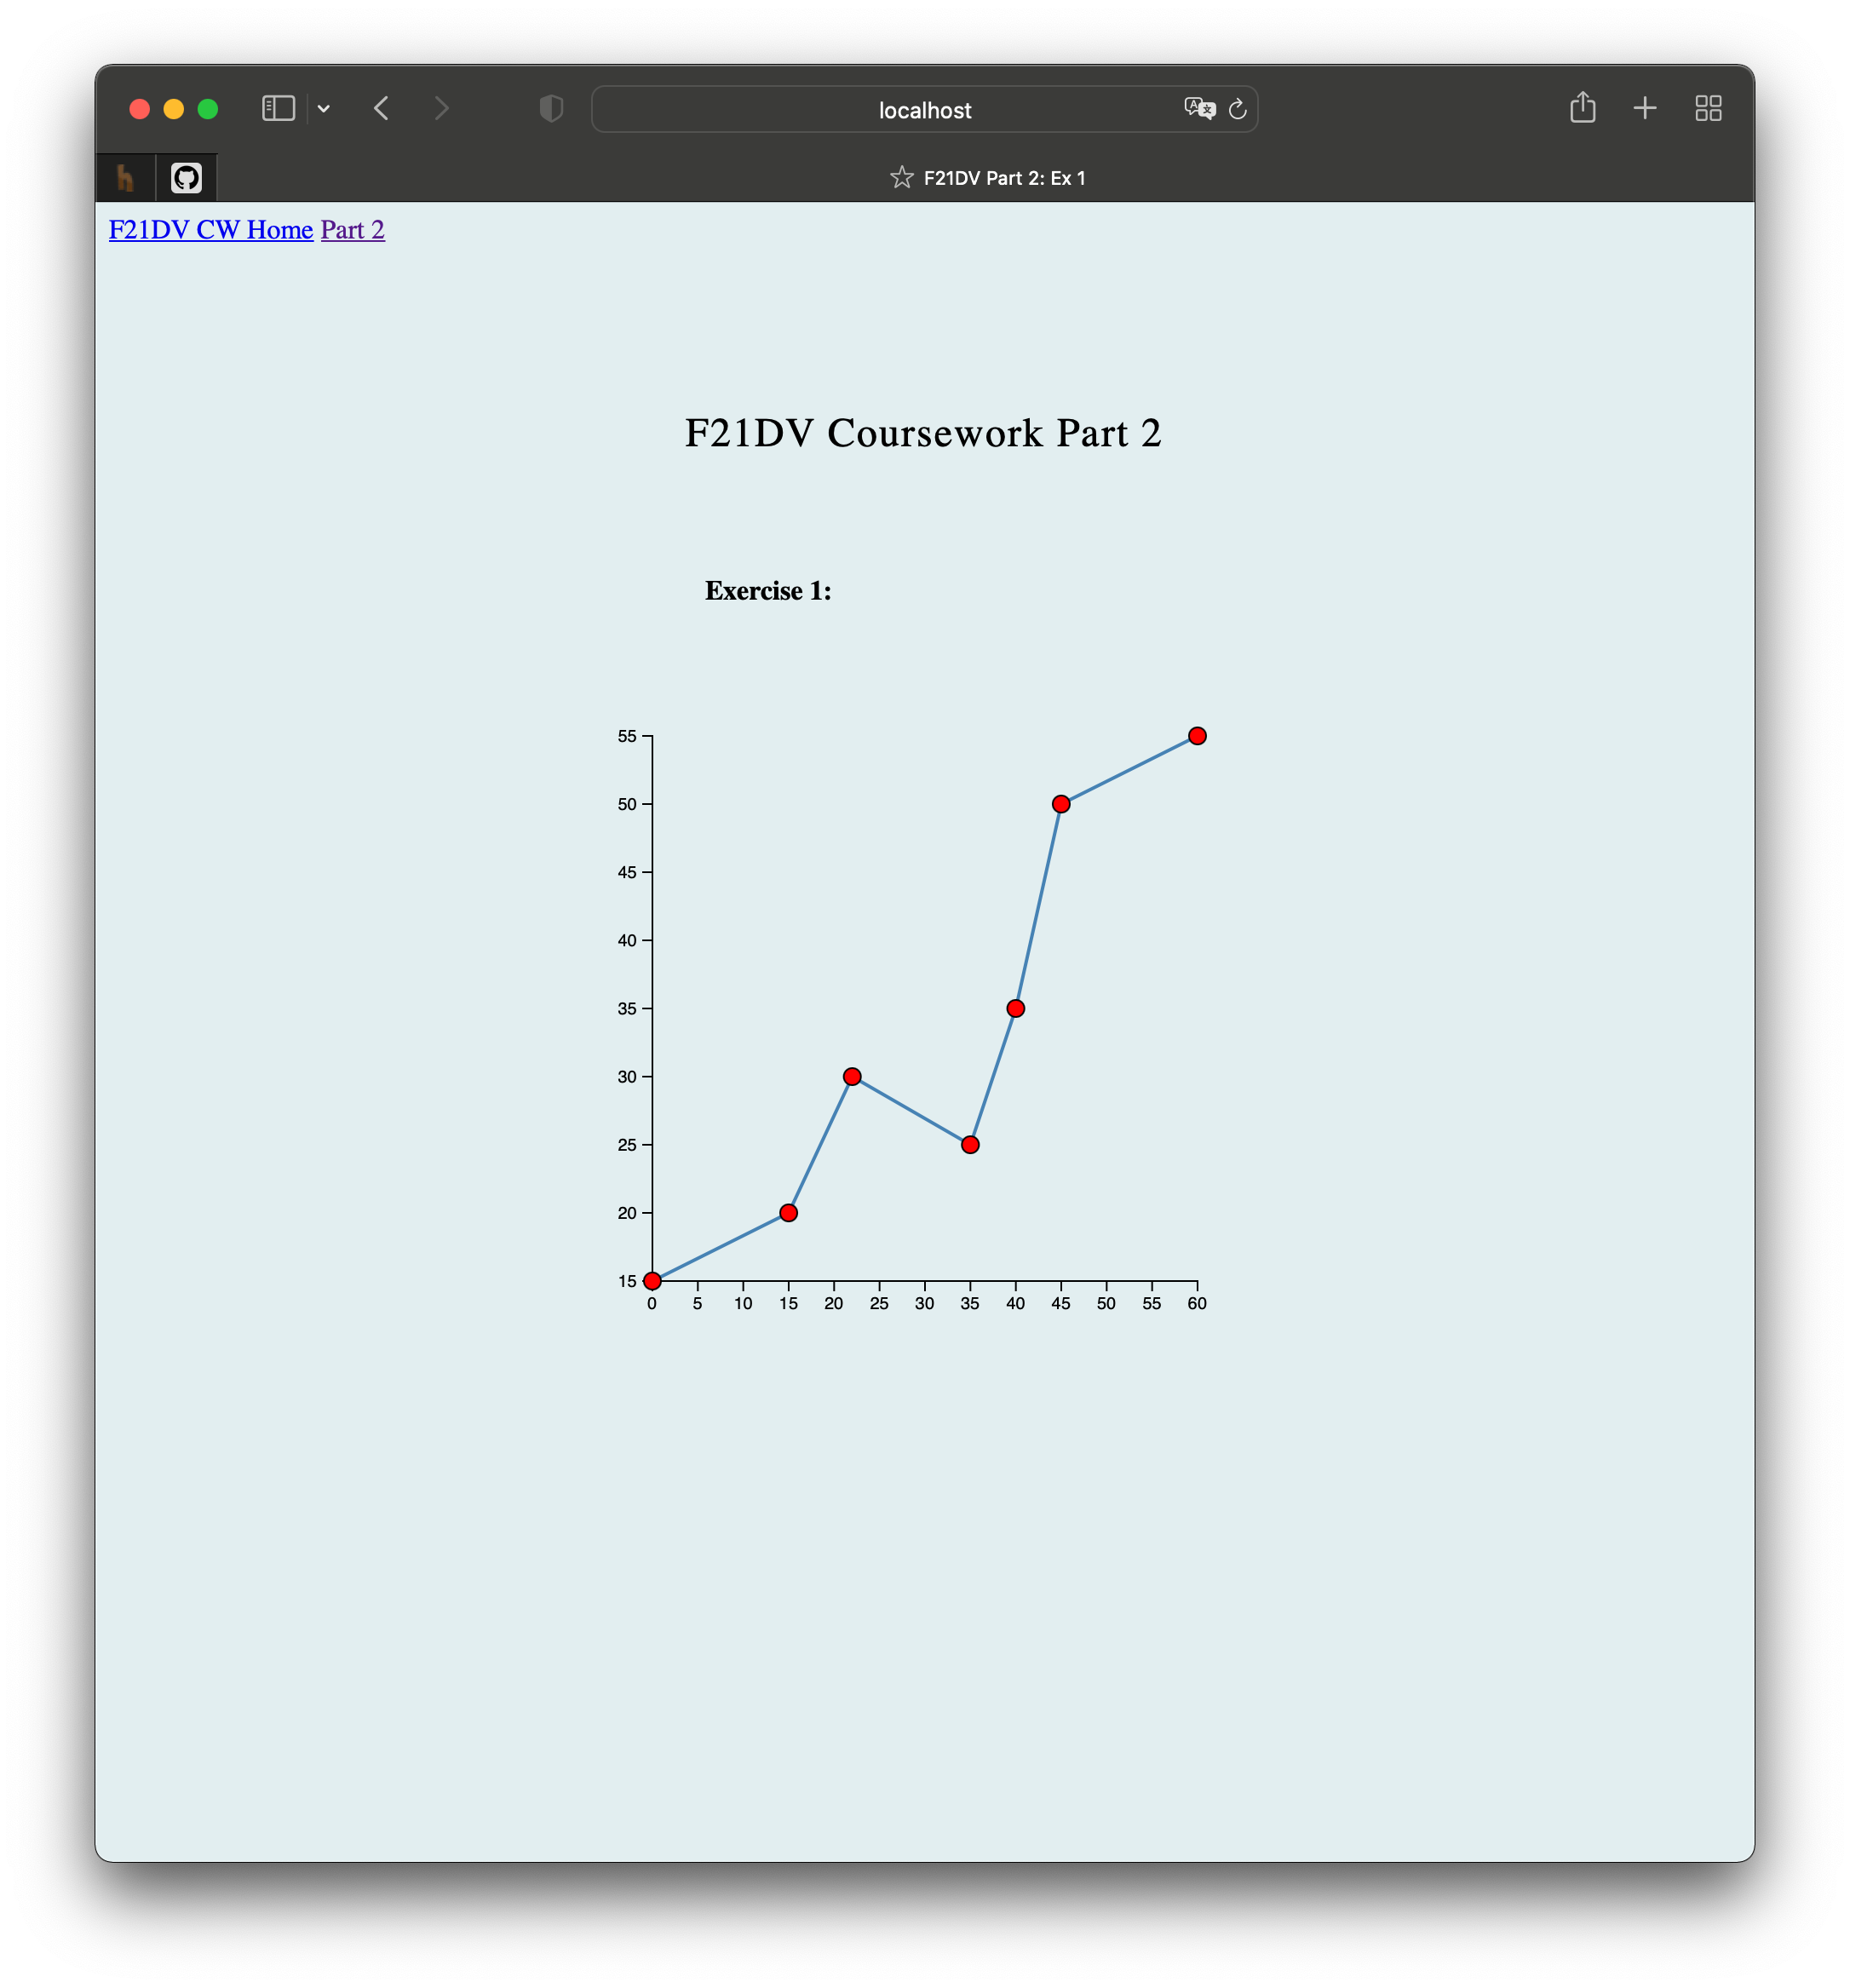
\includegraphics[width = 7.5cm]{images/ex1_1.png}
    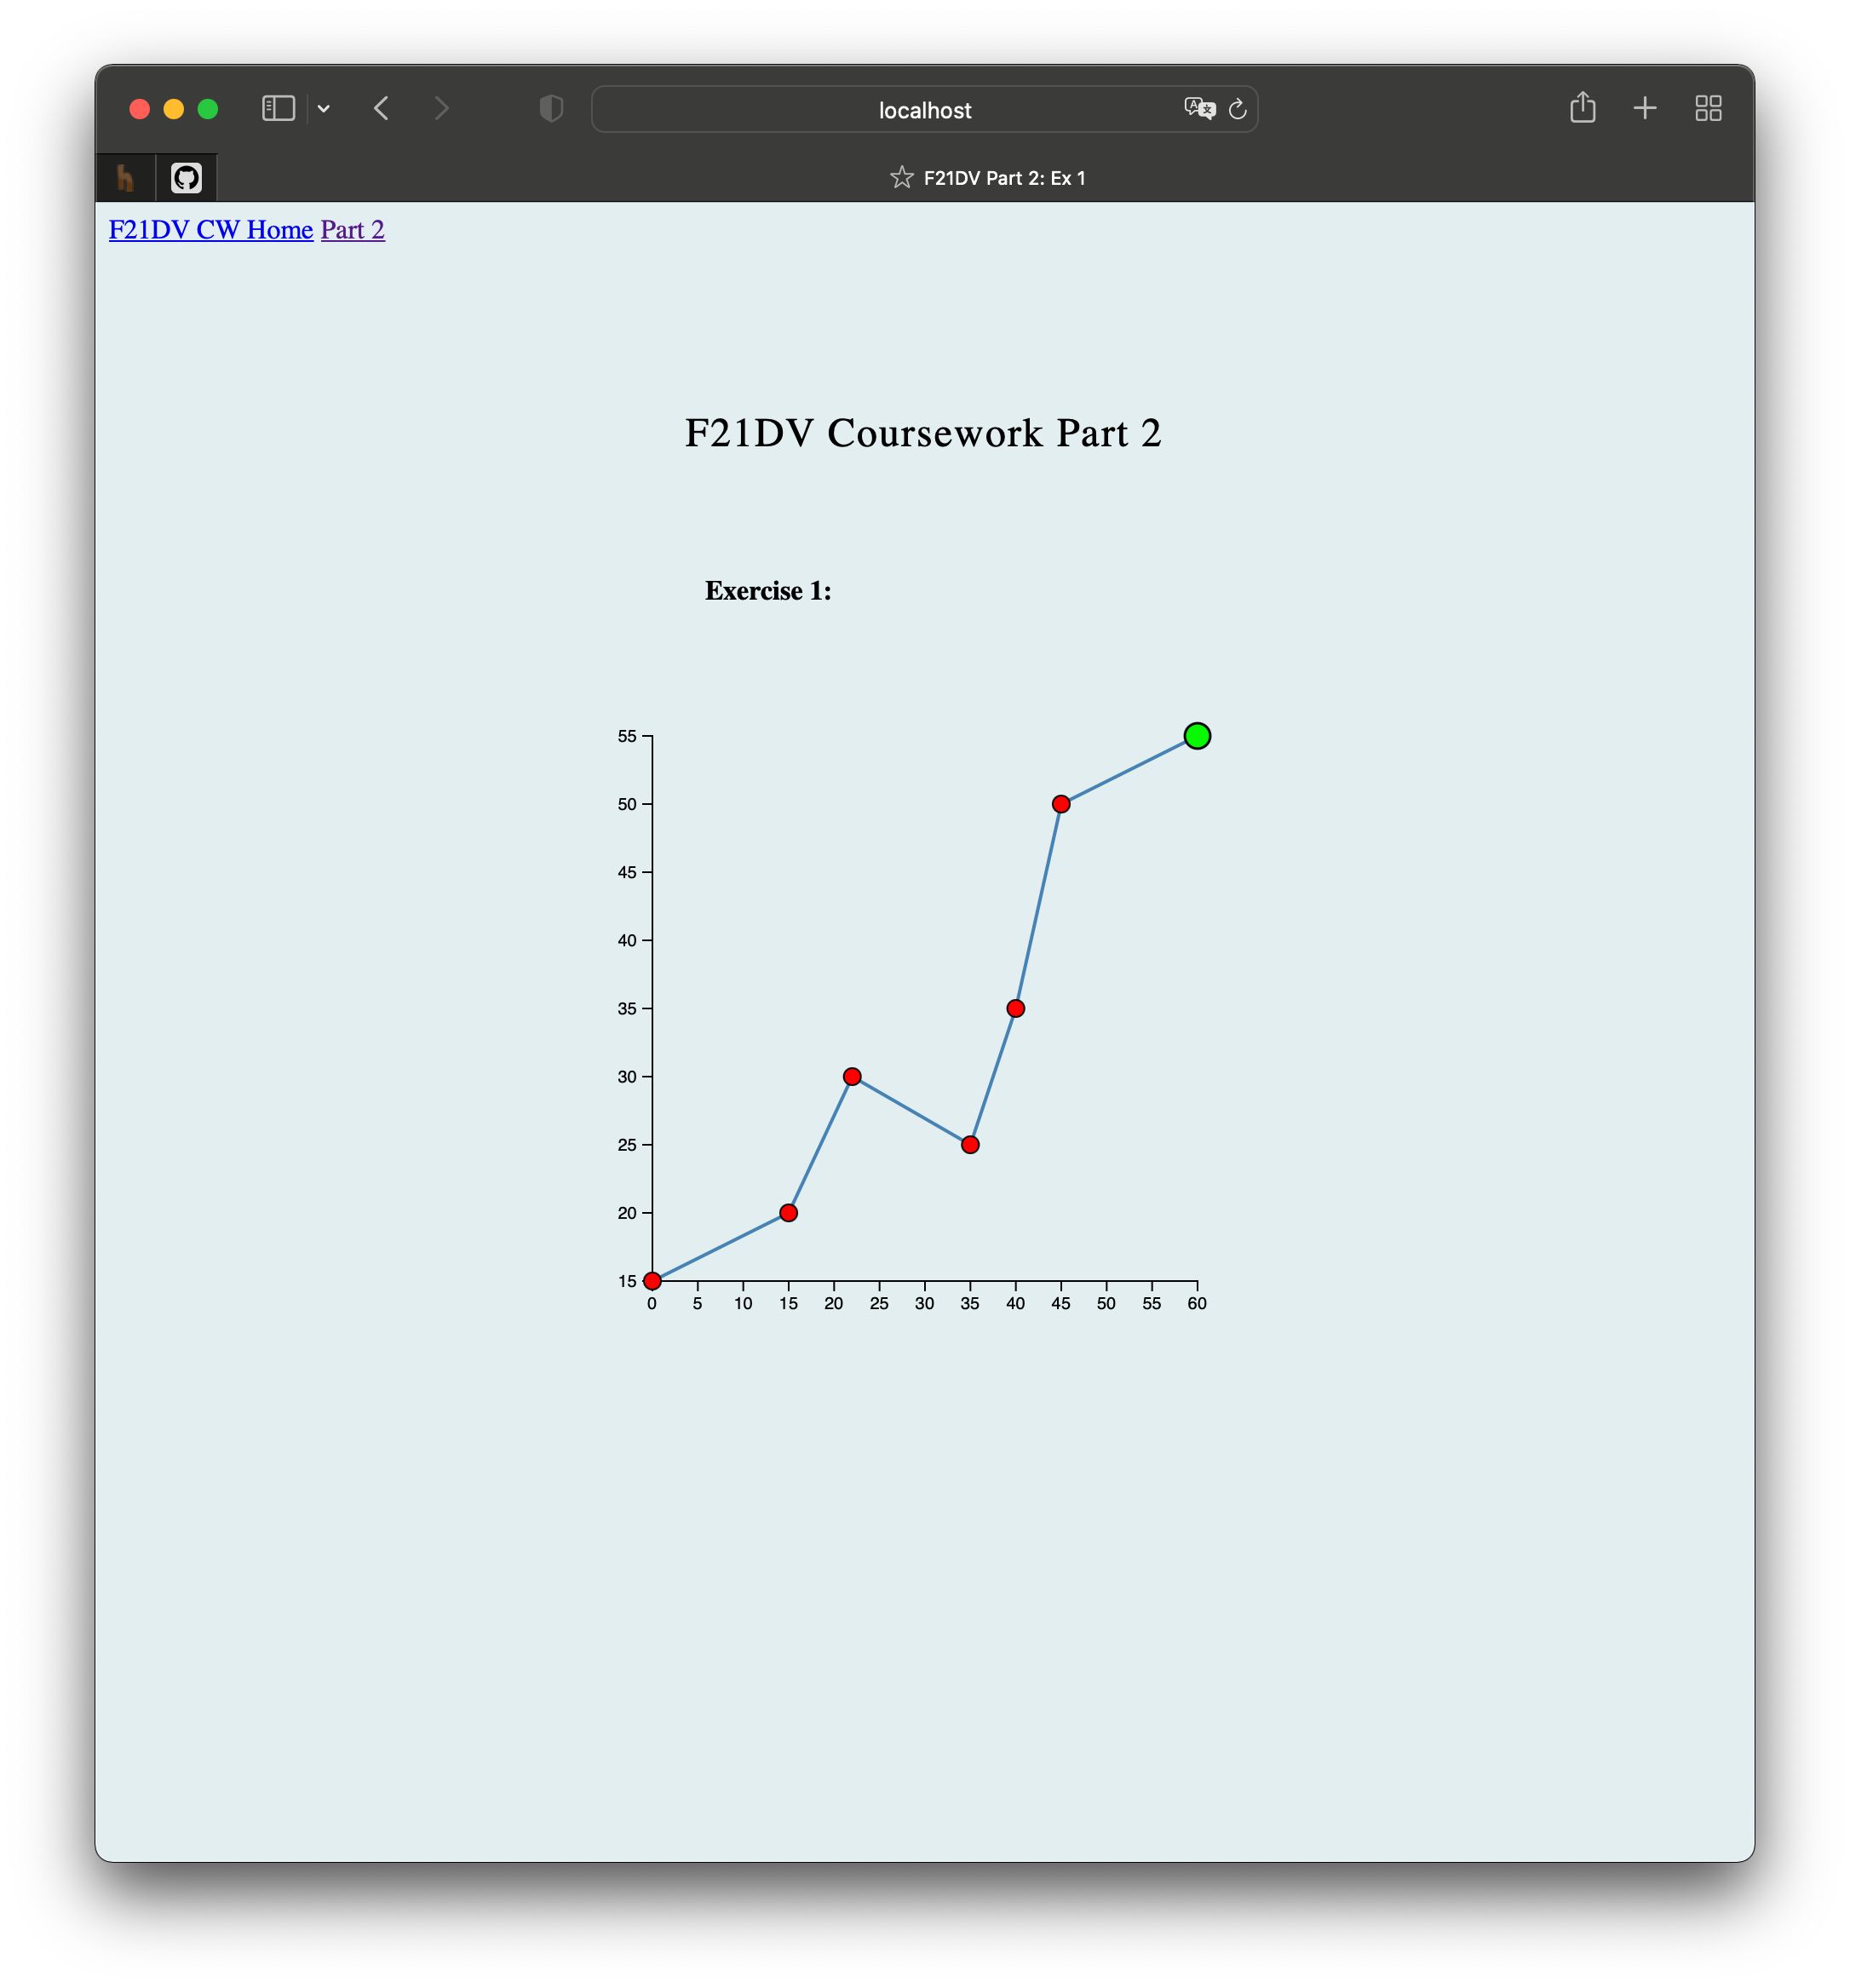
\includegraphics[width = 7.5cm]{images/ex1_2.png}
    \label{fig:ex1}
    \caption{Exercise 1}
\end{figure}
\FloatBarrier
Figure \ref{fig:ex1} shows a line chart with data points plotted on it. The right figure shows what happens when the mouse hovers upon a data point, the data point would pulse between red and green. *\textit{Can't seem to take a screenshot and capture the pointer}.

\newpage
\section{Exercise 2}
\begin{figure}[!ht]
    \centering
    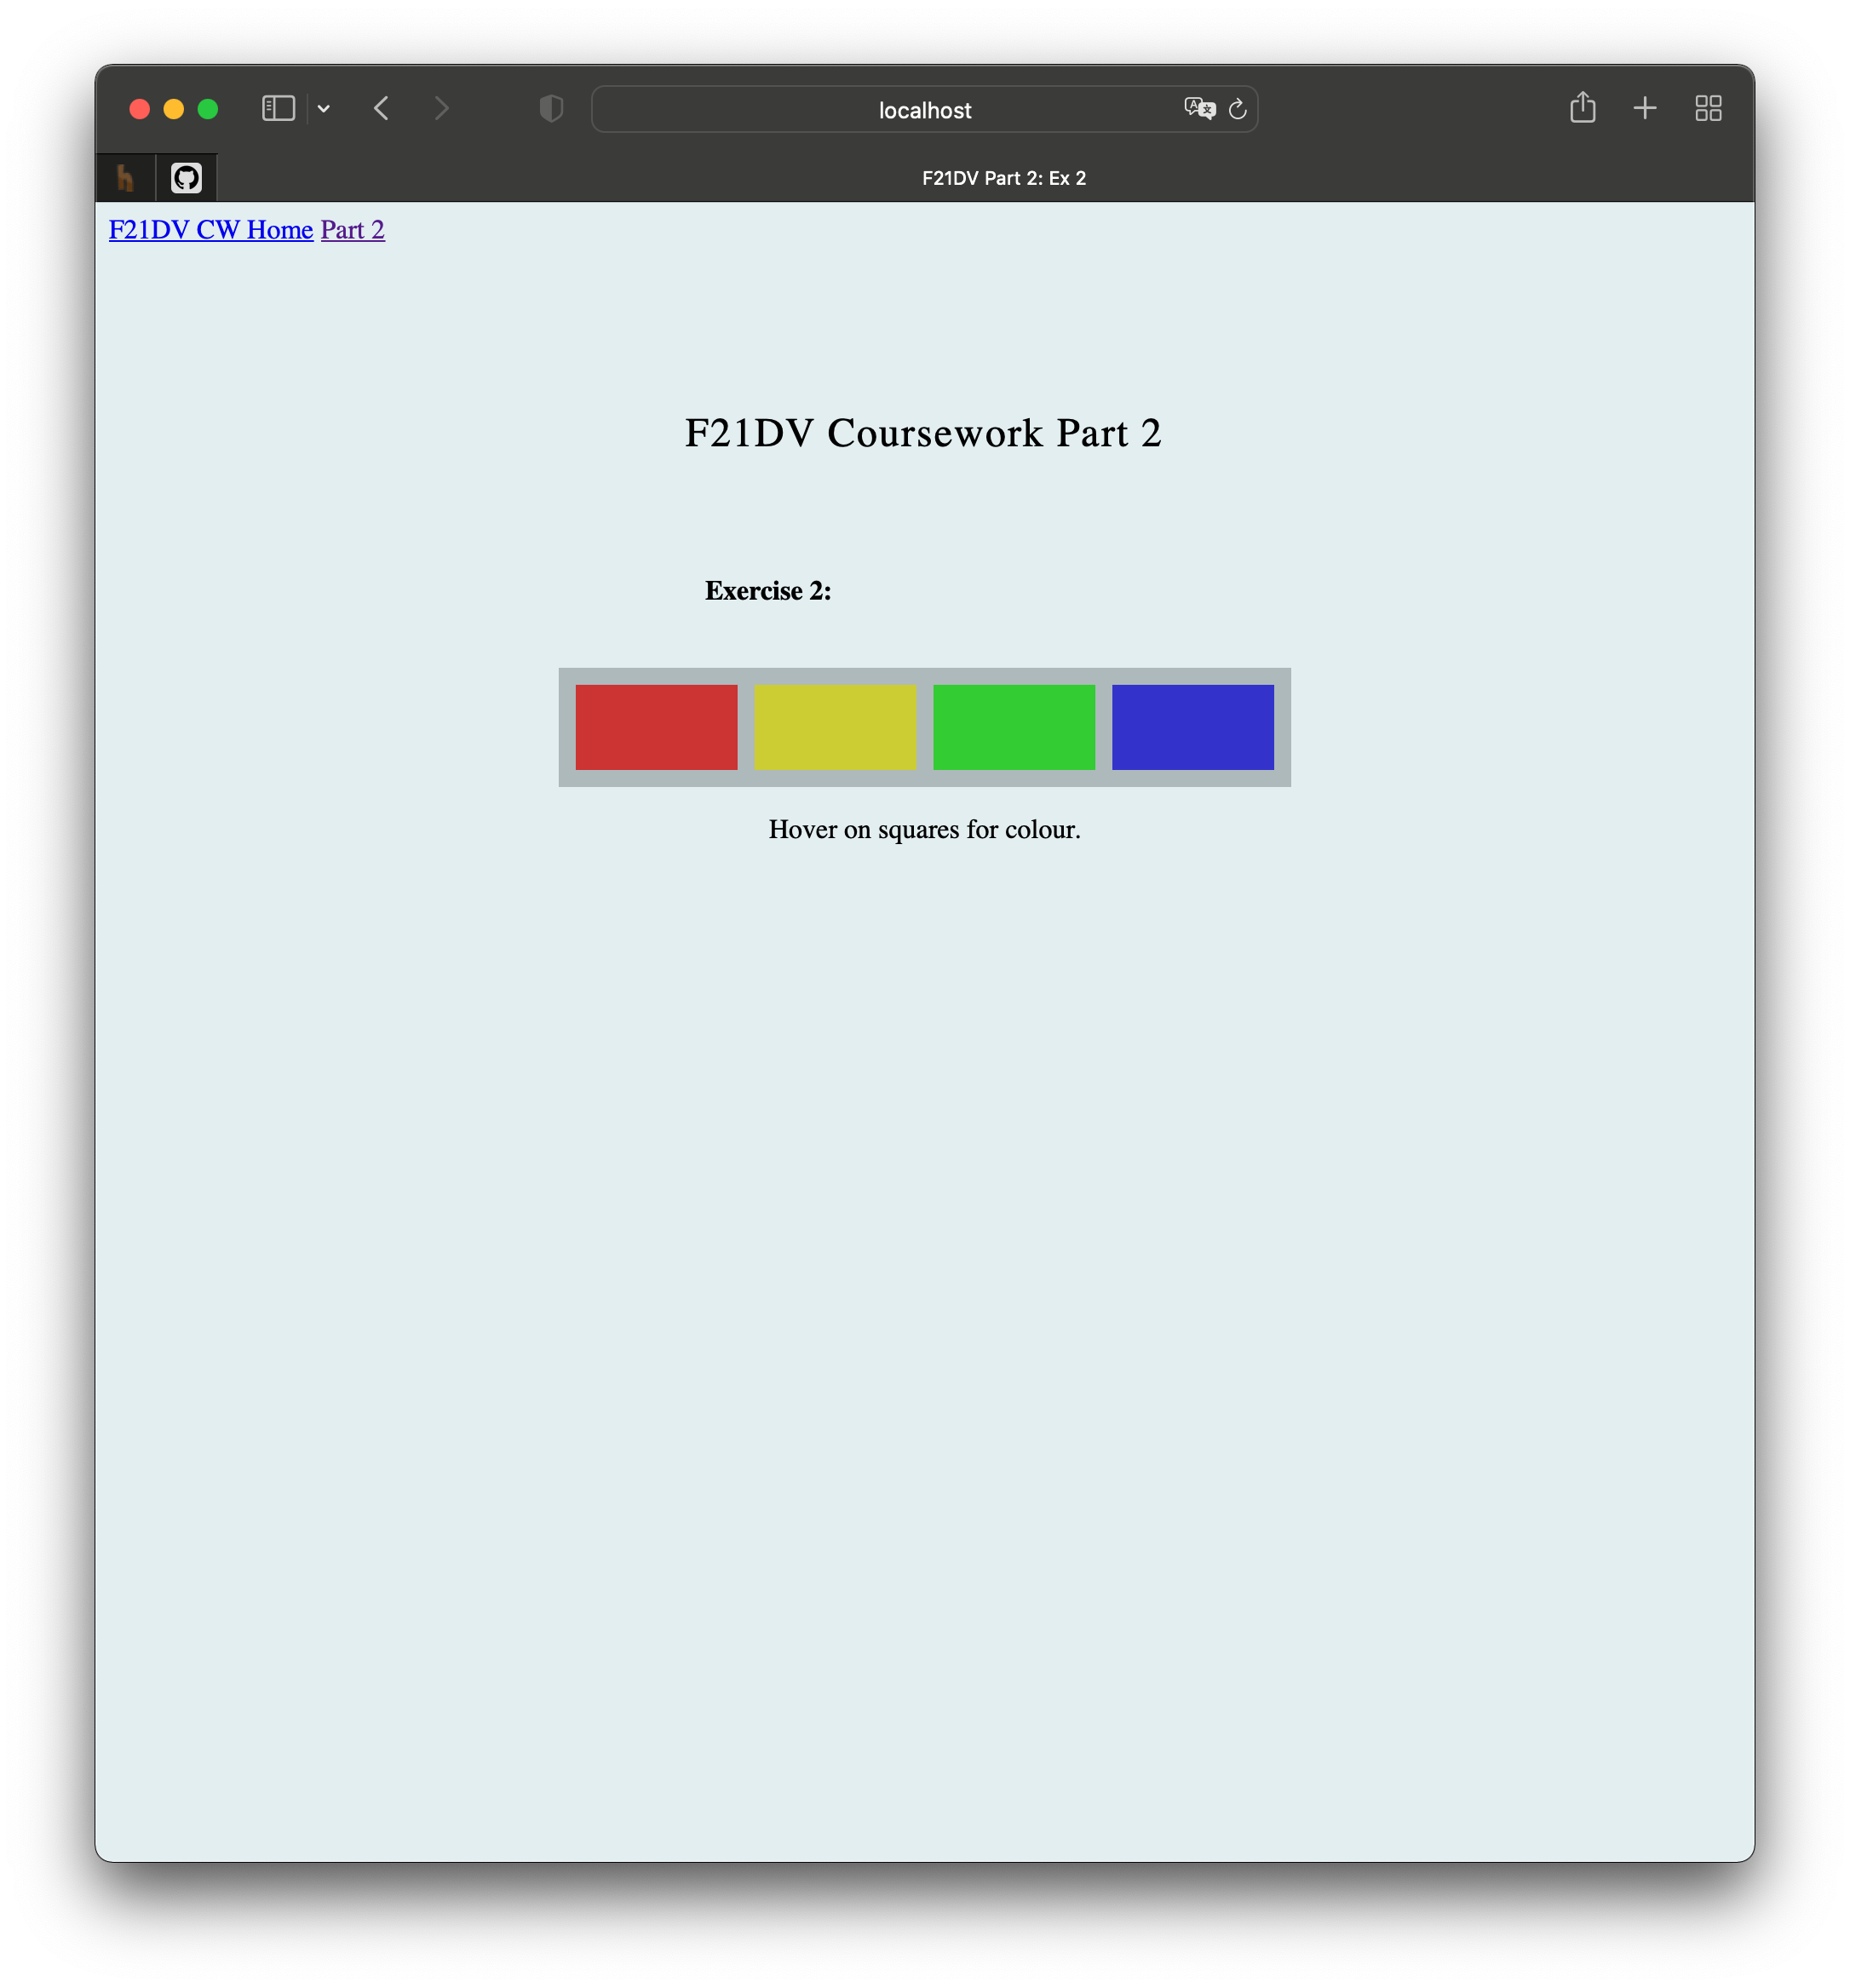
\includegraphics[width = 7.5cm]{images/ex2_1.png}
    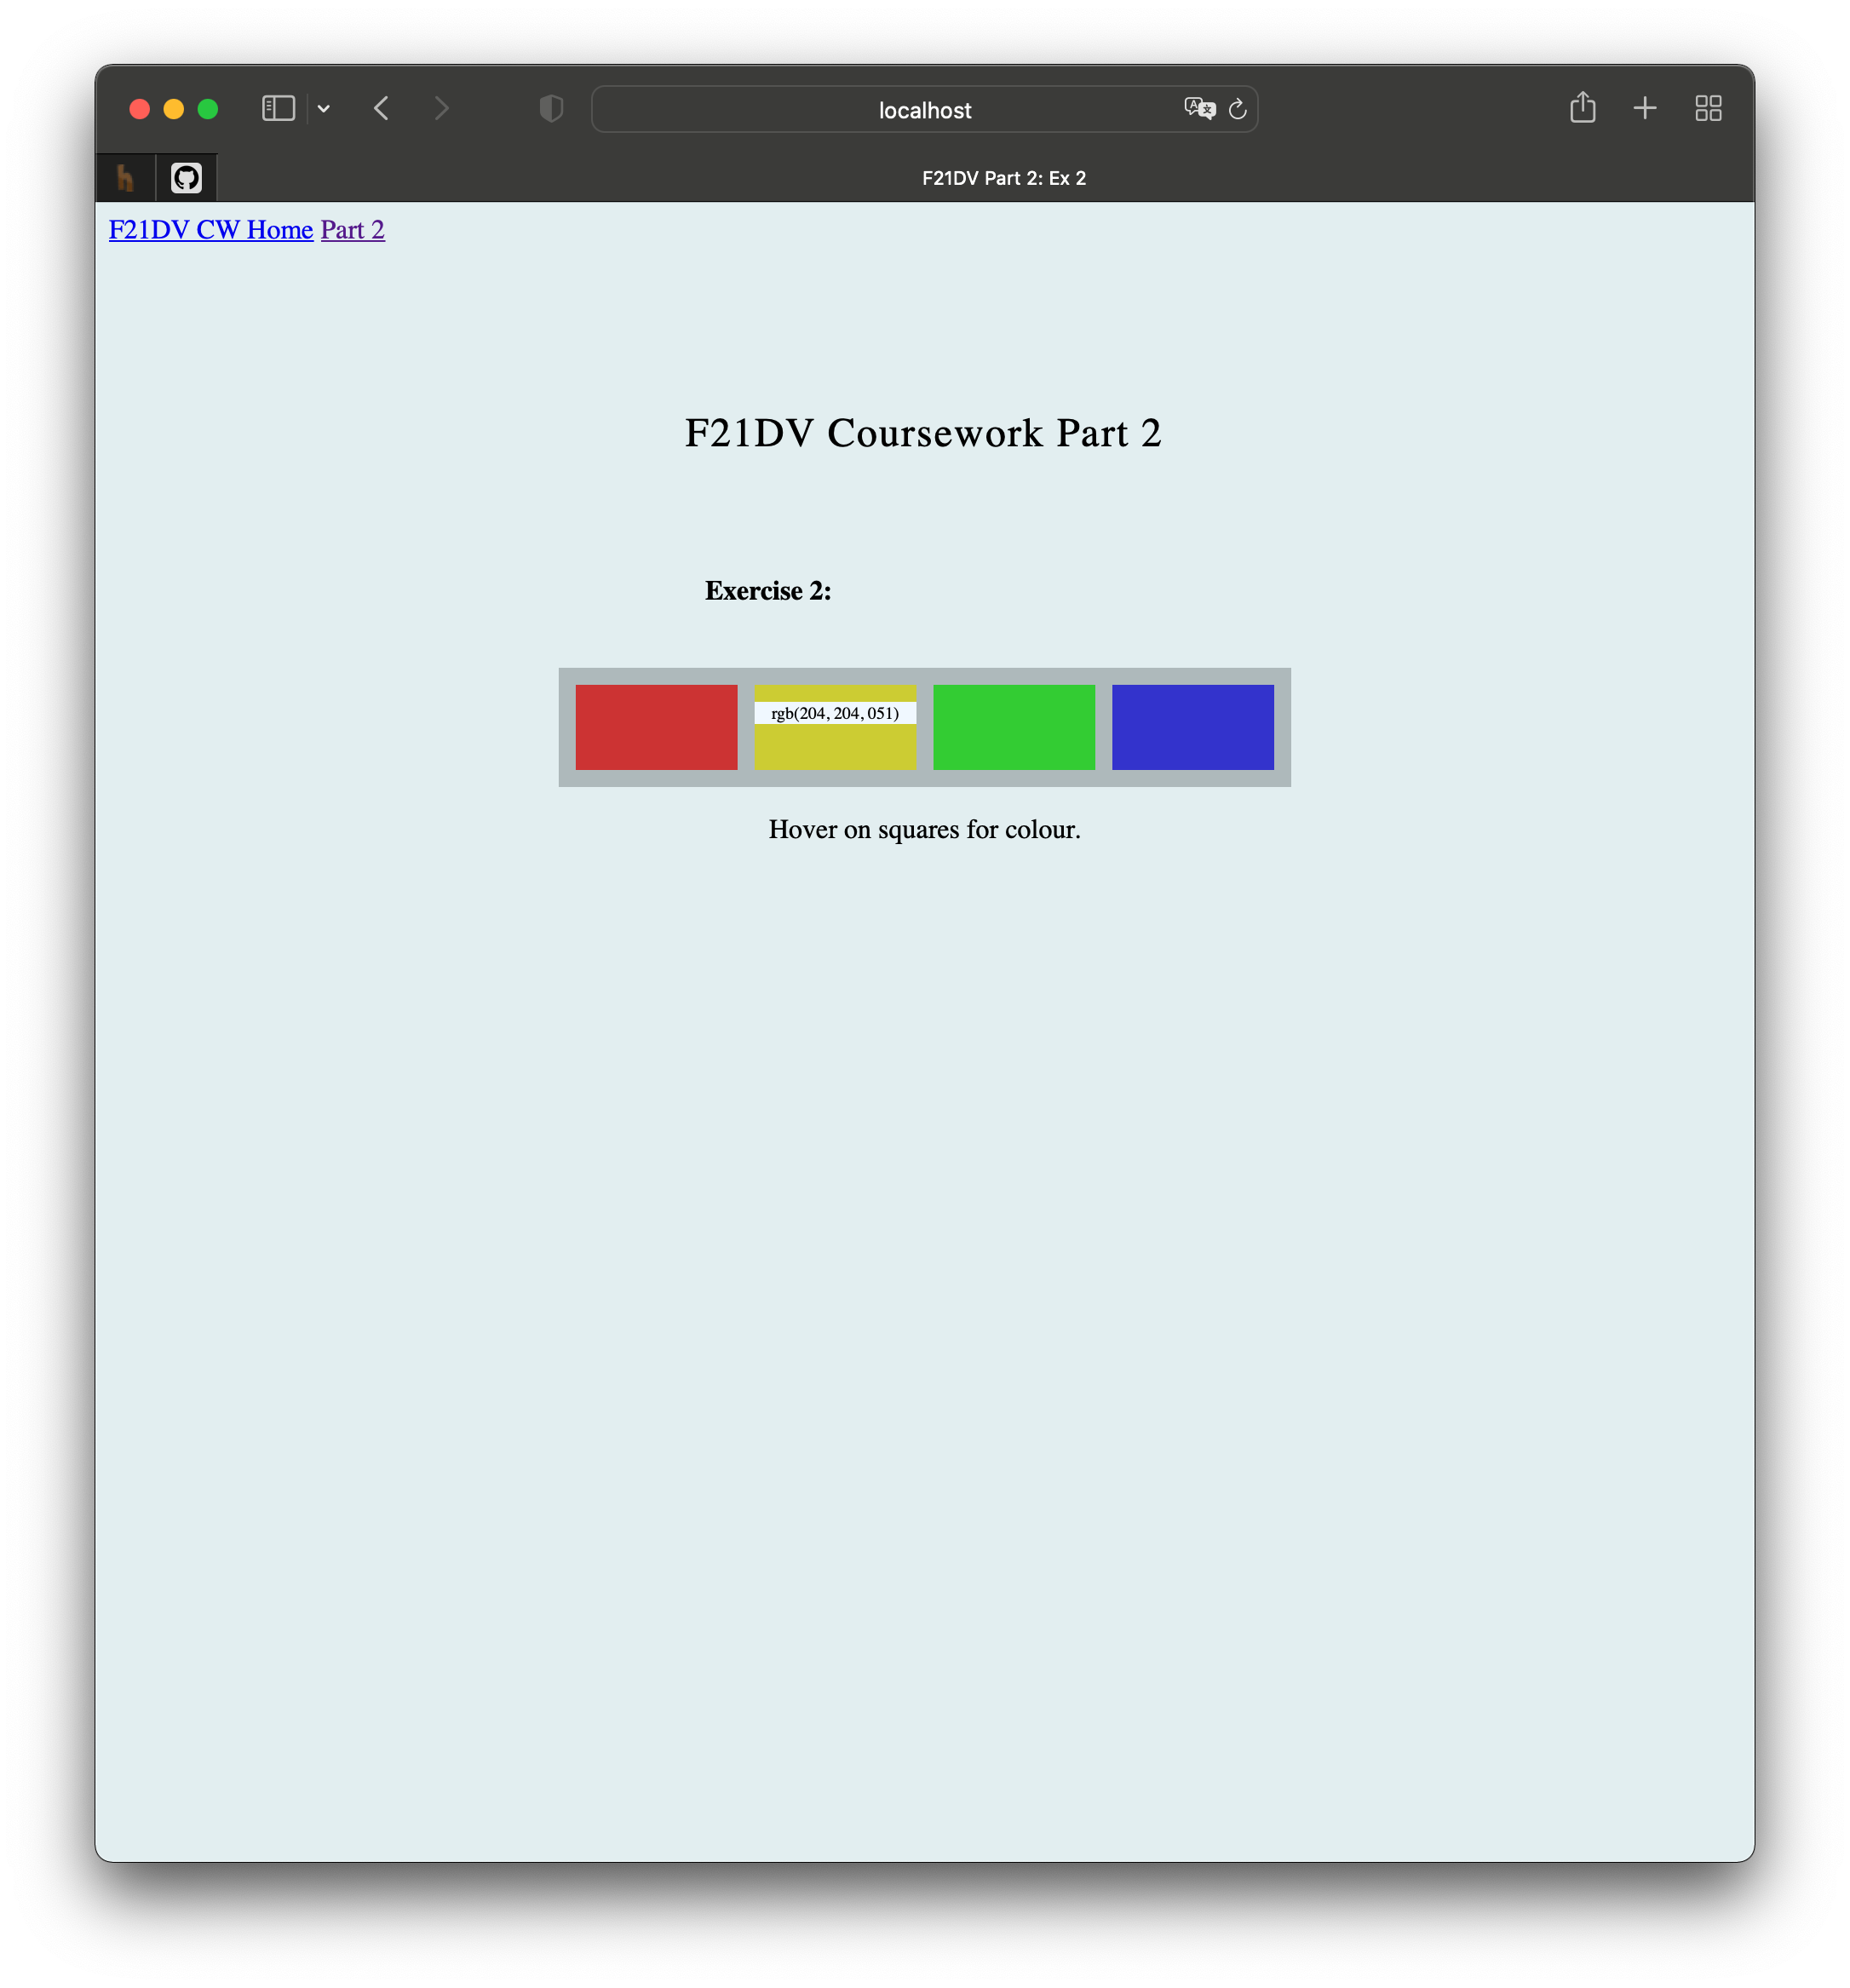
\includegraphics[width = 7.5cm]{images/ex2_2.png}
    \label{fig:ex2}
    \caption{Exercise 2}
\end{figure}
\FloatBarrier
% \lstinputlisting[language=JavaScript]{../../public/js/part2/task2.js}
Figure \ref{fig:ex2} shows 4 blocks with different colours. The blocks are just a div defined within a grid. Each block also has a fill colour defined using the \verb|Rgb()| colour method, as shown in line 10. Upon hovering the mouse on the div, the div would show a text element displaying the Rgb colour. This effect is done using the css \verb|:hover| method.

\newpage
\section{Exercise 3}
\begin{figure}[!ht]
    \centering
    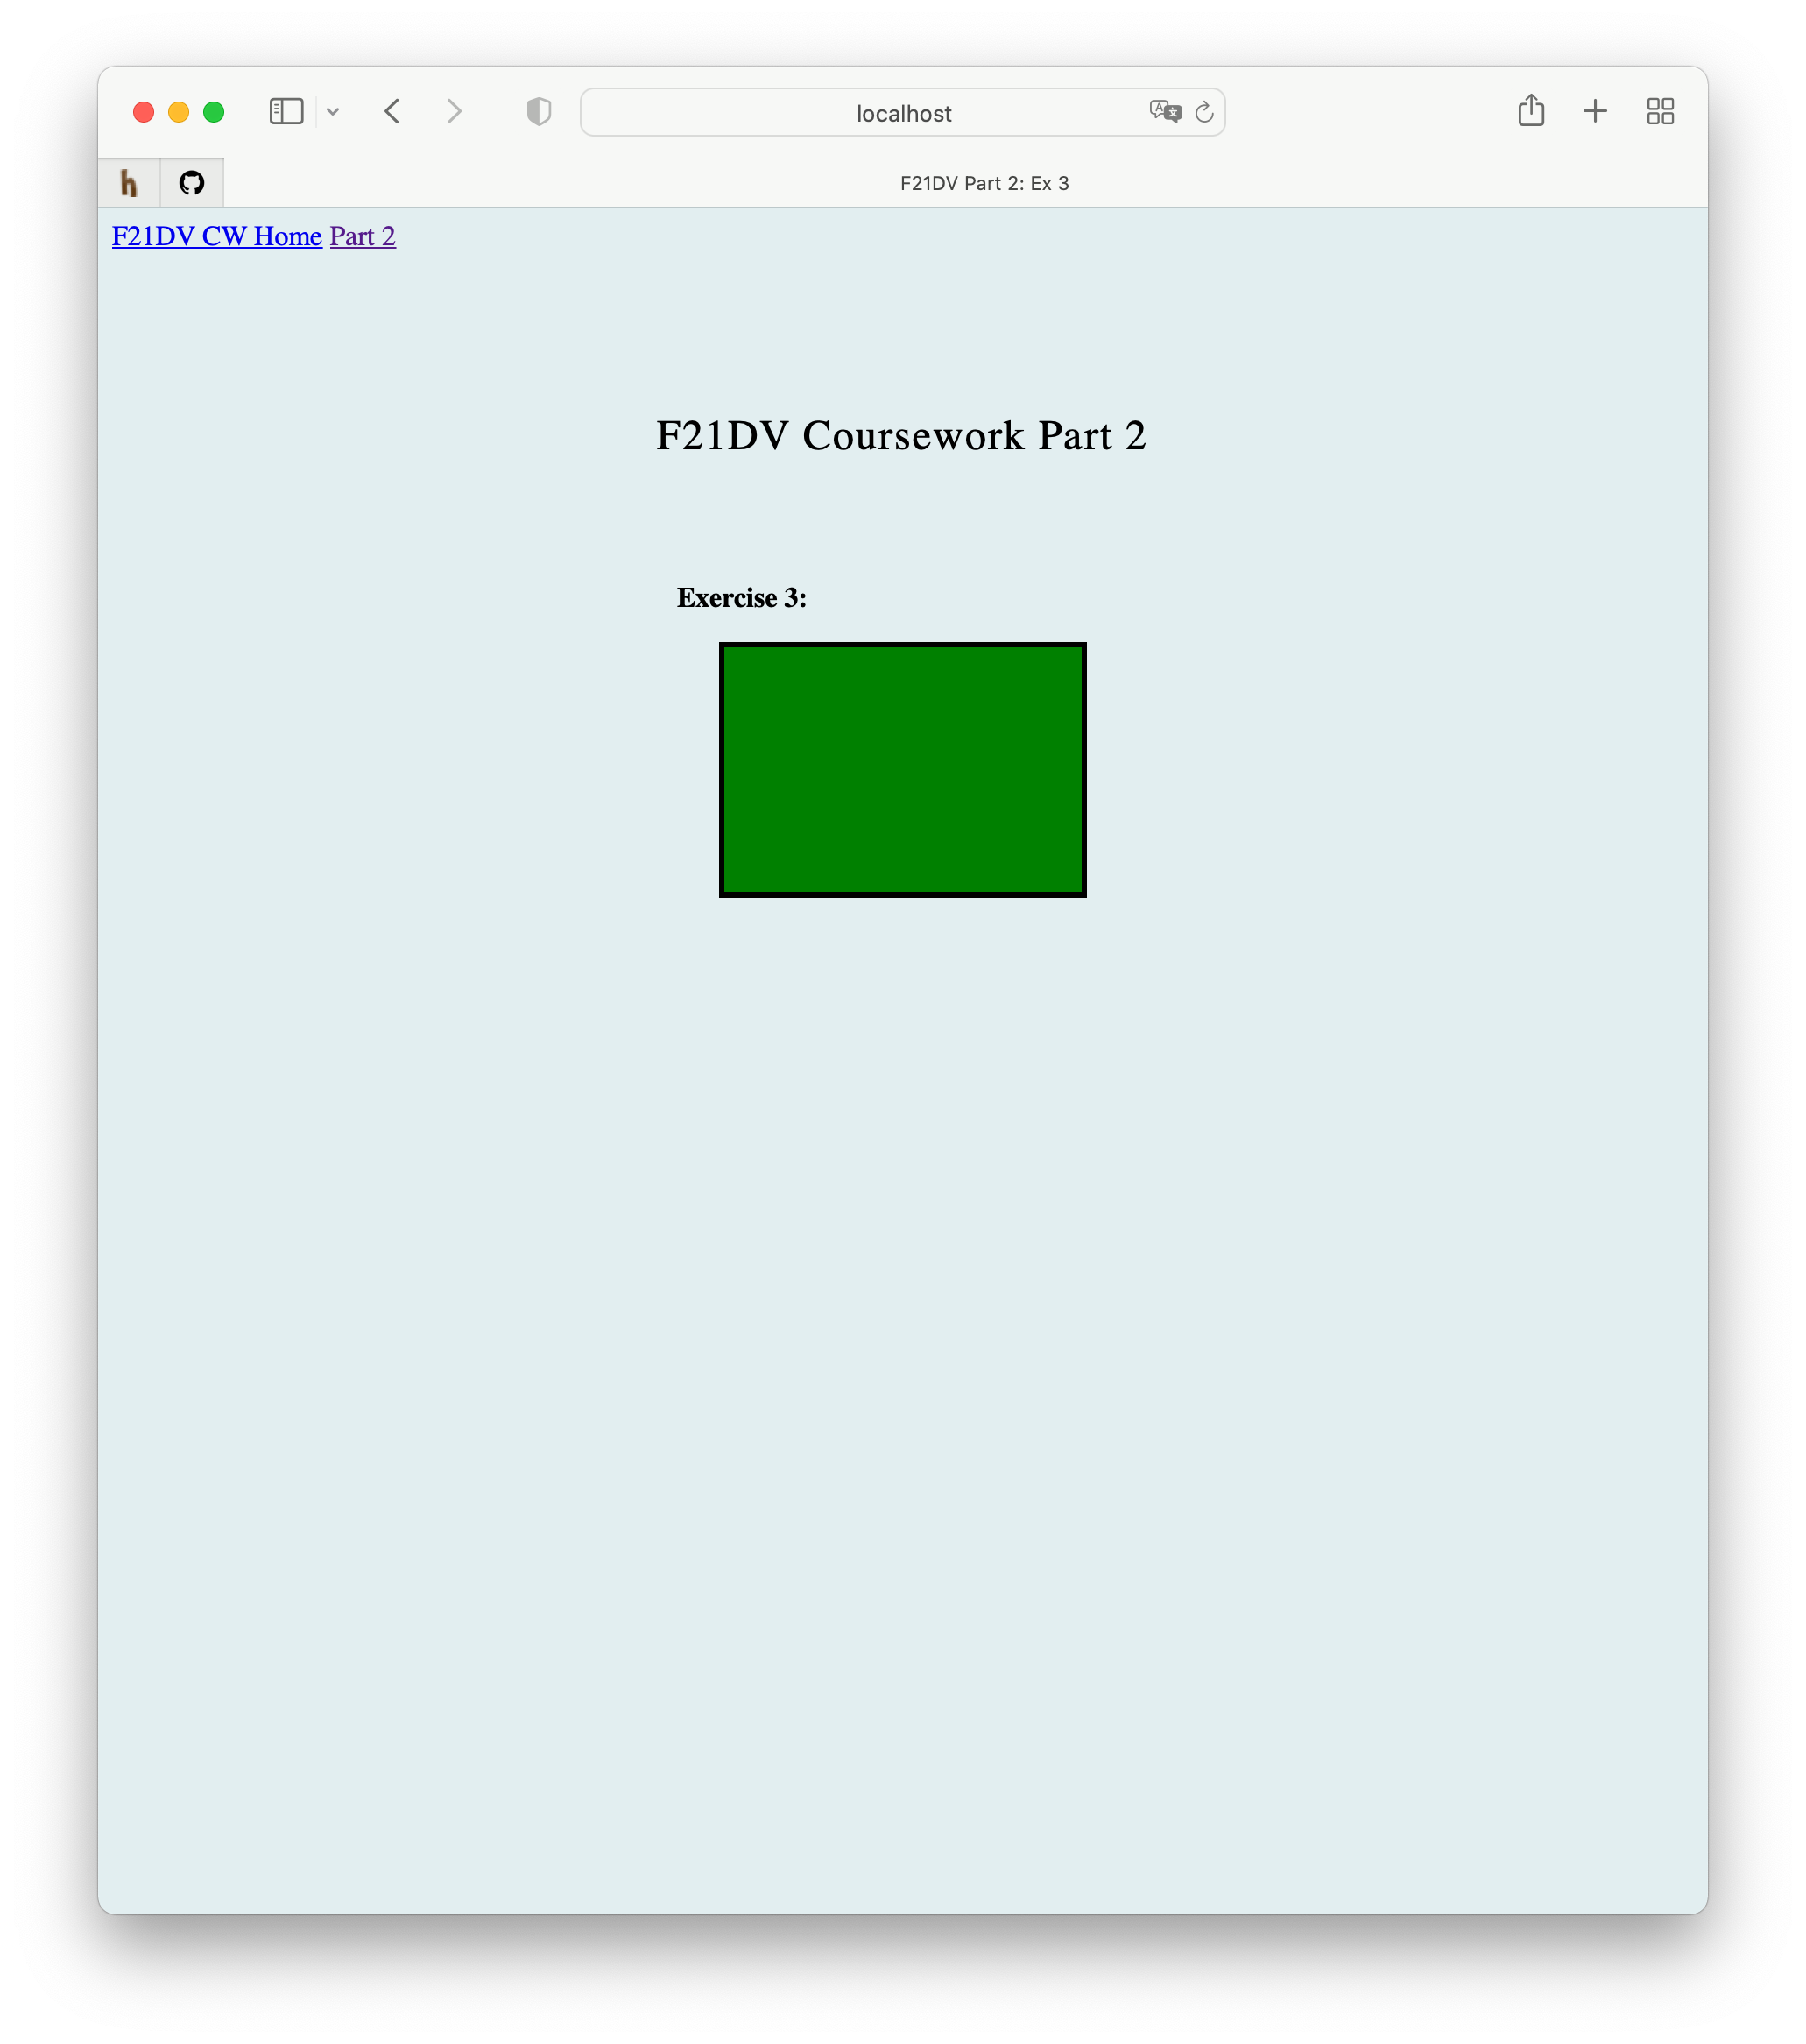
\includegraphics[width = 7cm]{images/ex3_1.png}
    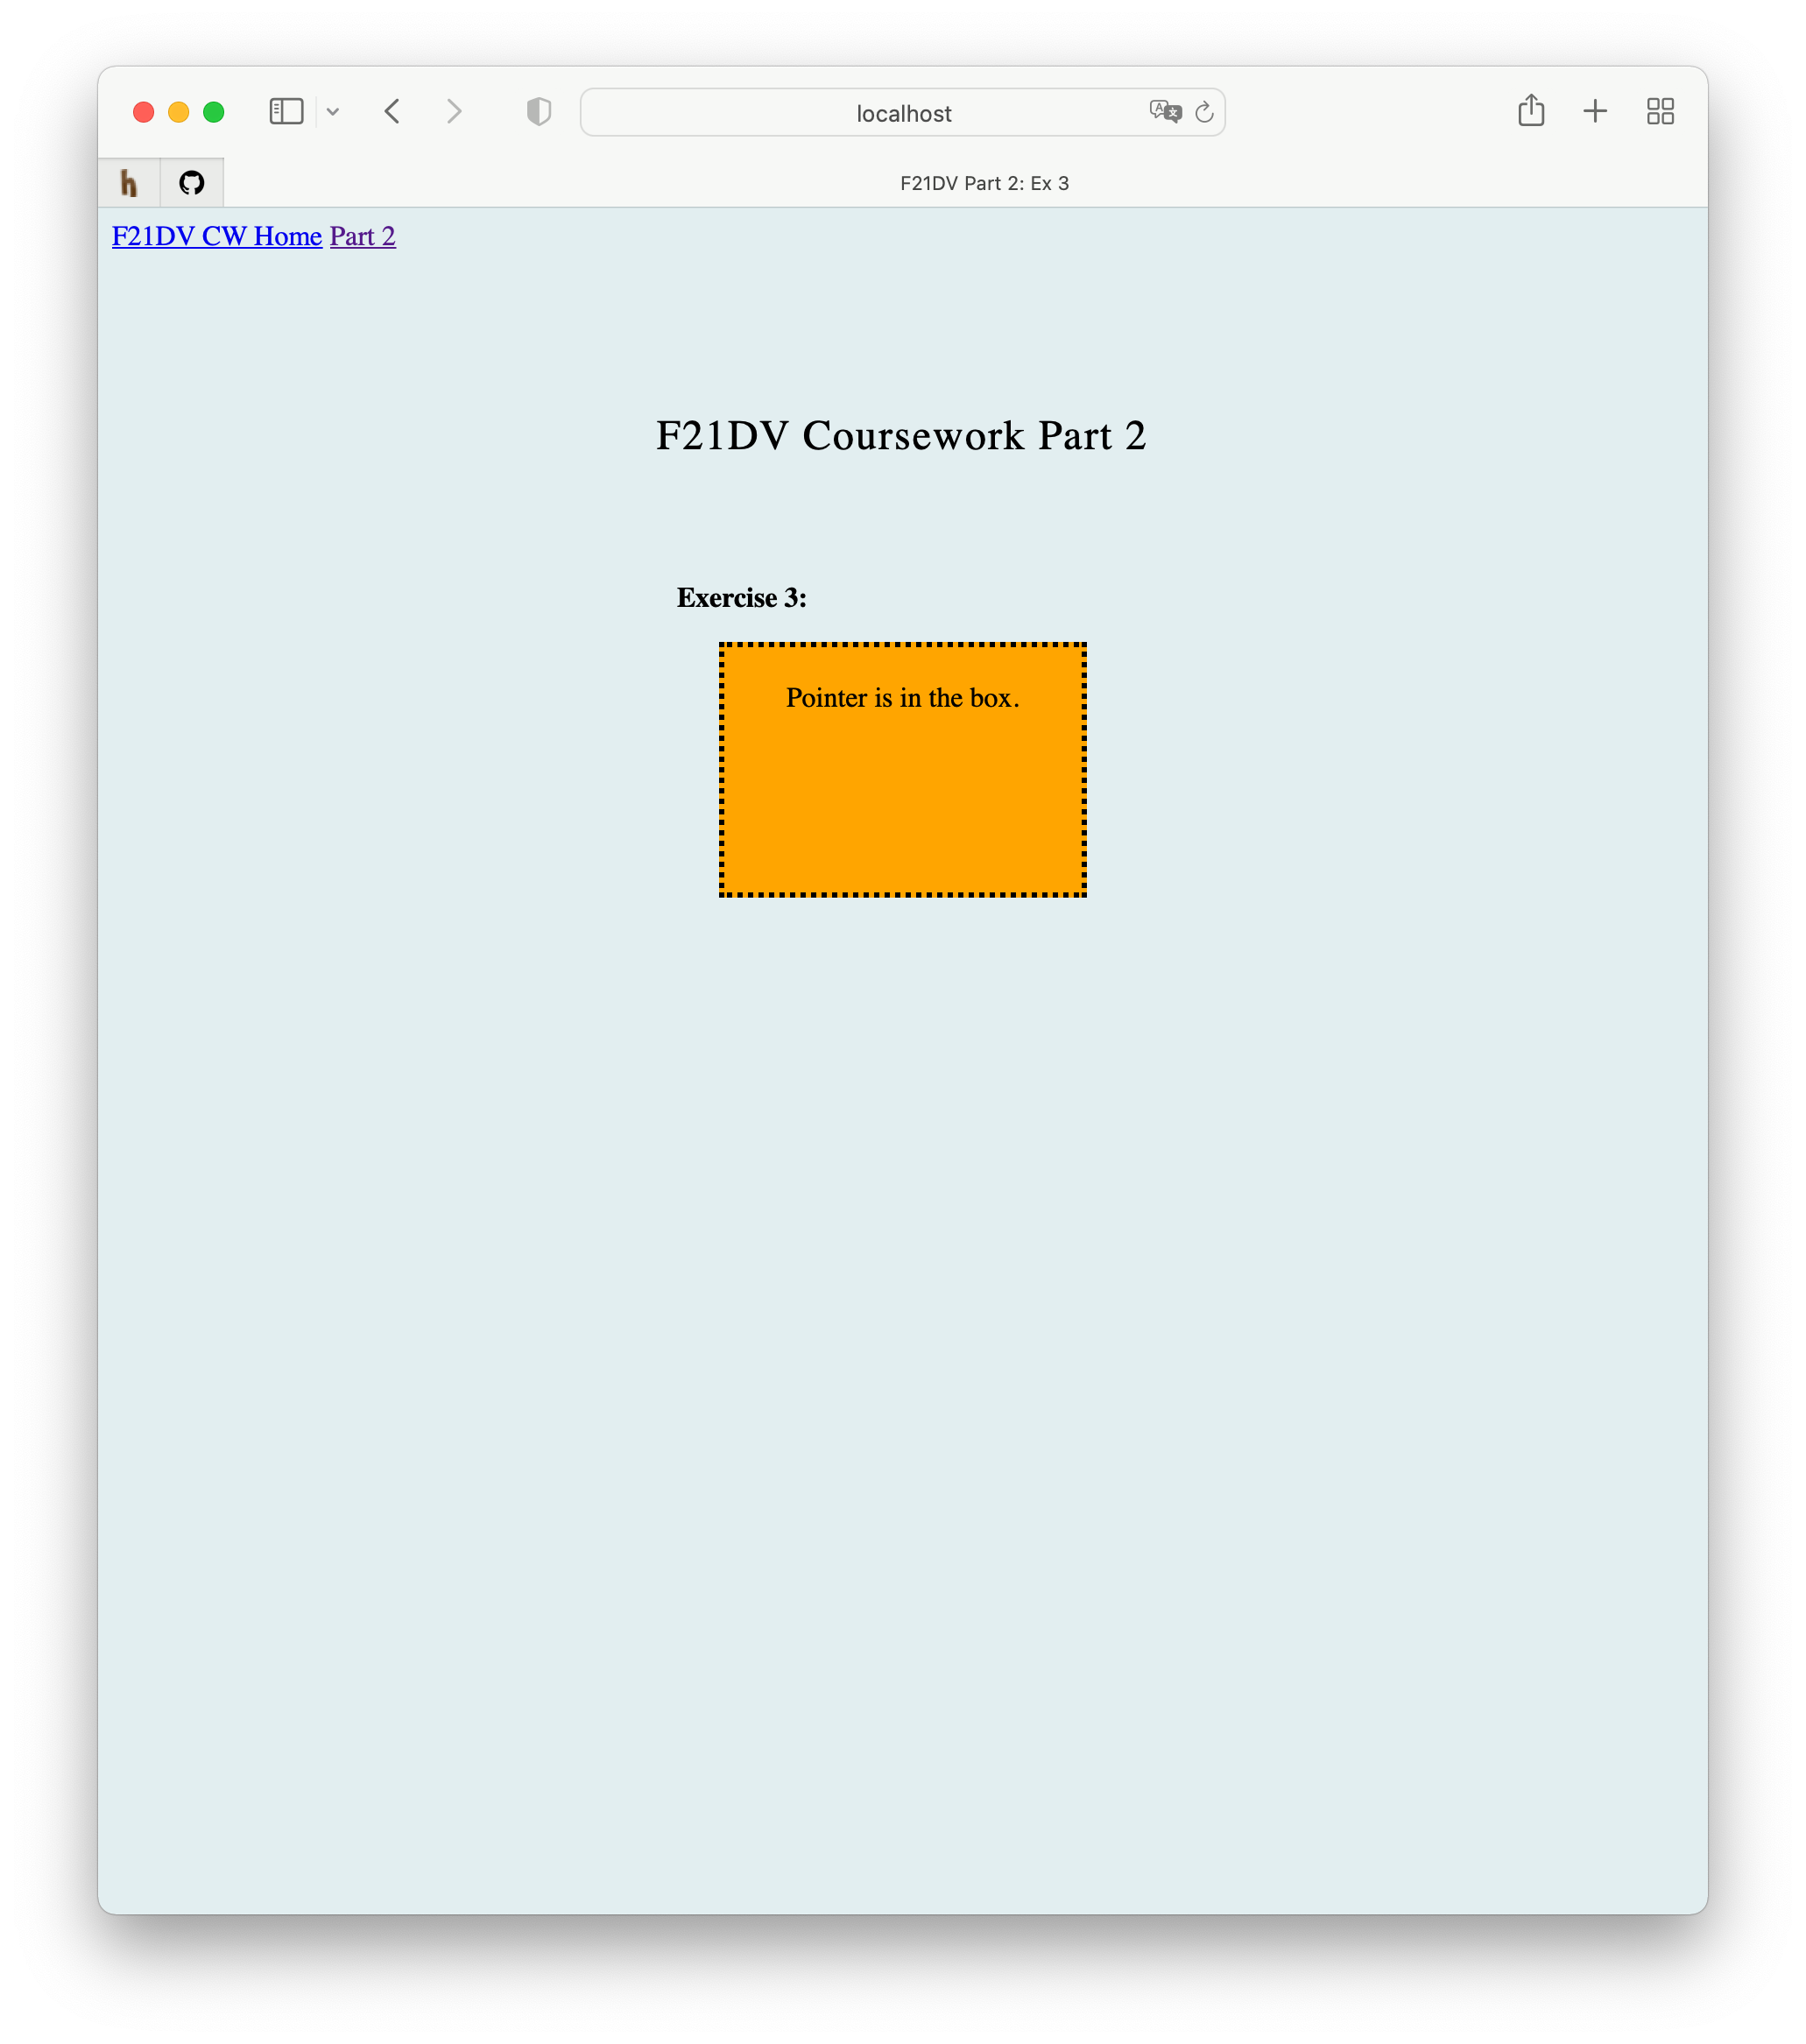
\includegraphics[width = 7cm]{images/ex3_2.png}
    \label{fig:ex3}
    \caption{Exercise 3}
\end{figure}
\FloatBarrier
\lstinputlisting[language=JavaScript]{../../public/js/part2/task3.js}
Figure \ref{fig:ex3} shows a block thats green colour. Upon mouse hover on the box, the box now shows a text that says `Pointer is in the box', its colour is now orange, and it has a new type of border. This is done using the \verb|.on()| function.

\newpage
\section{Exercise 4}
\begin{figure}[!ht]
    \centering
    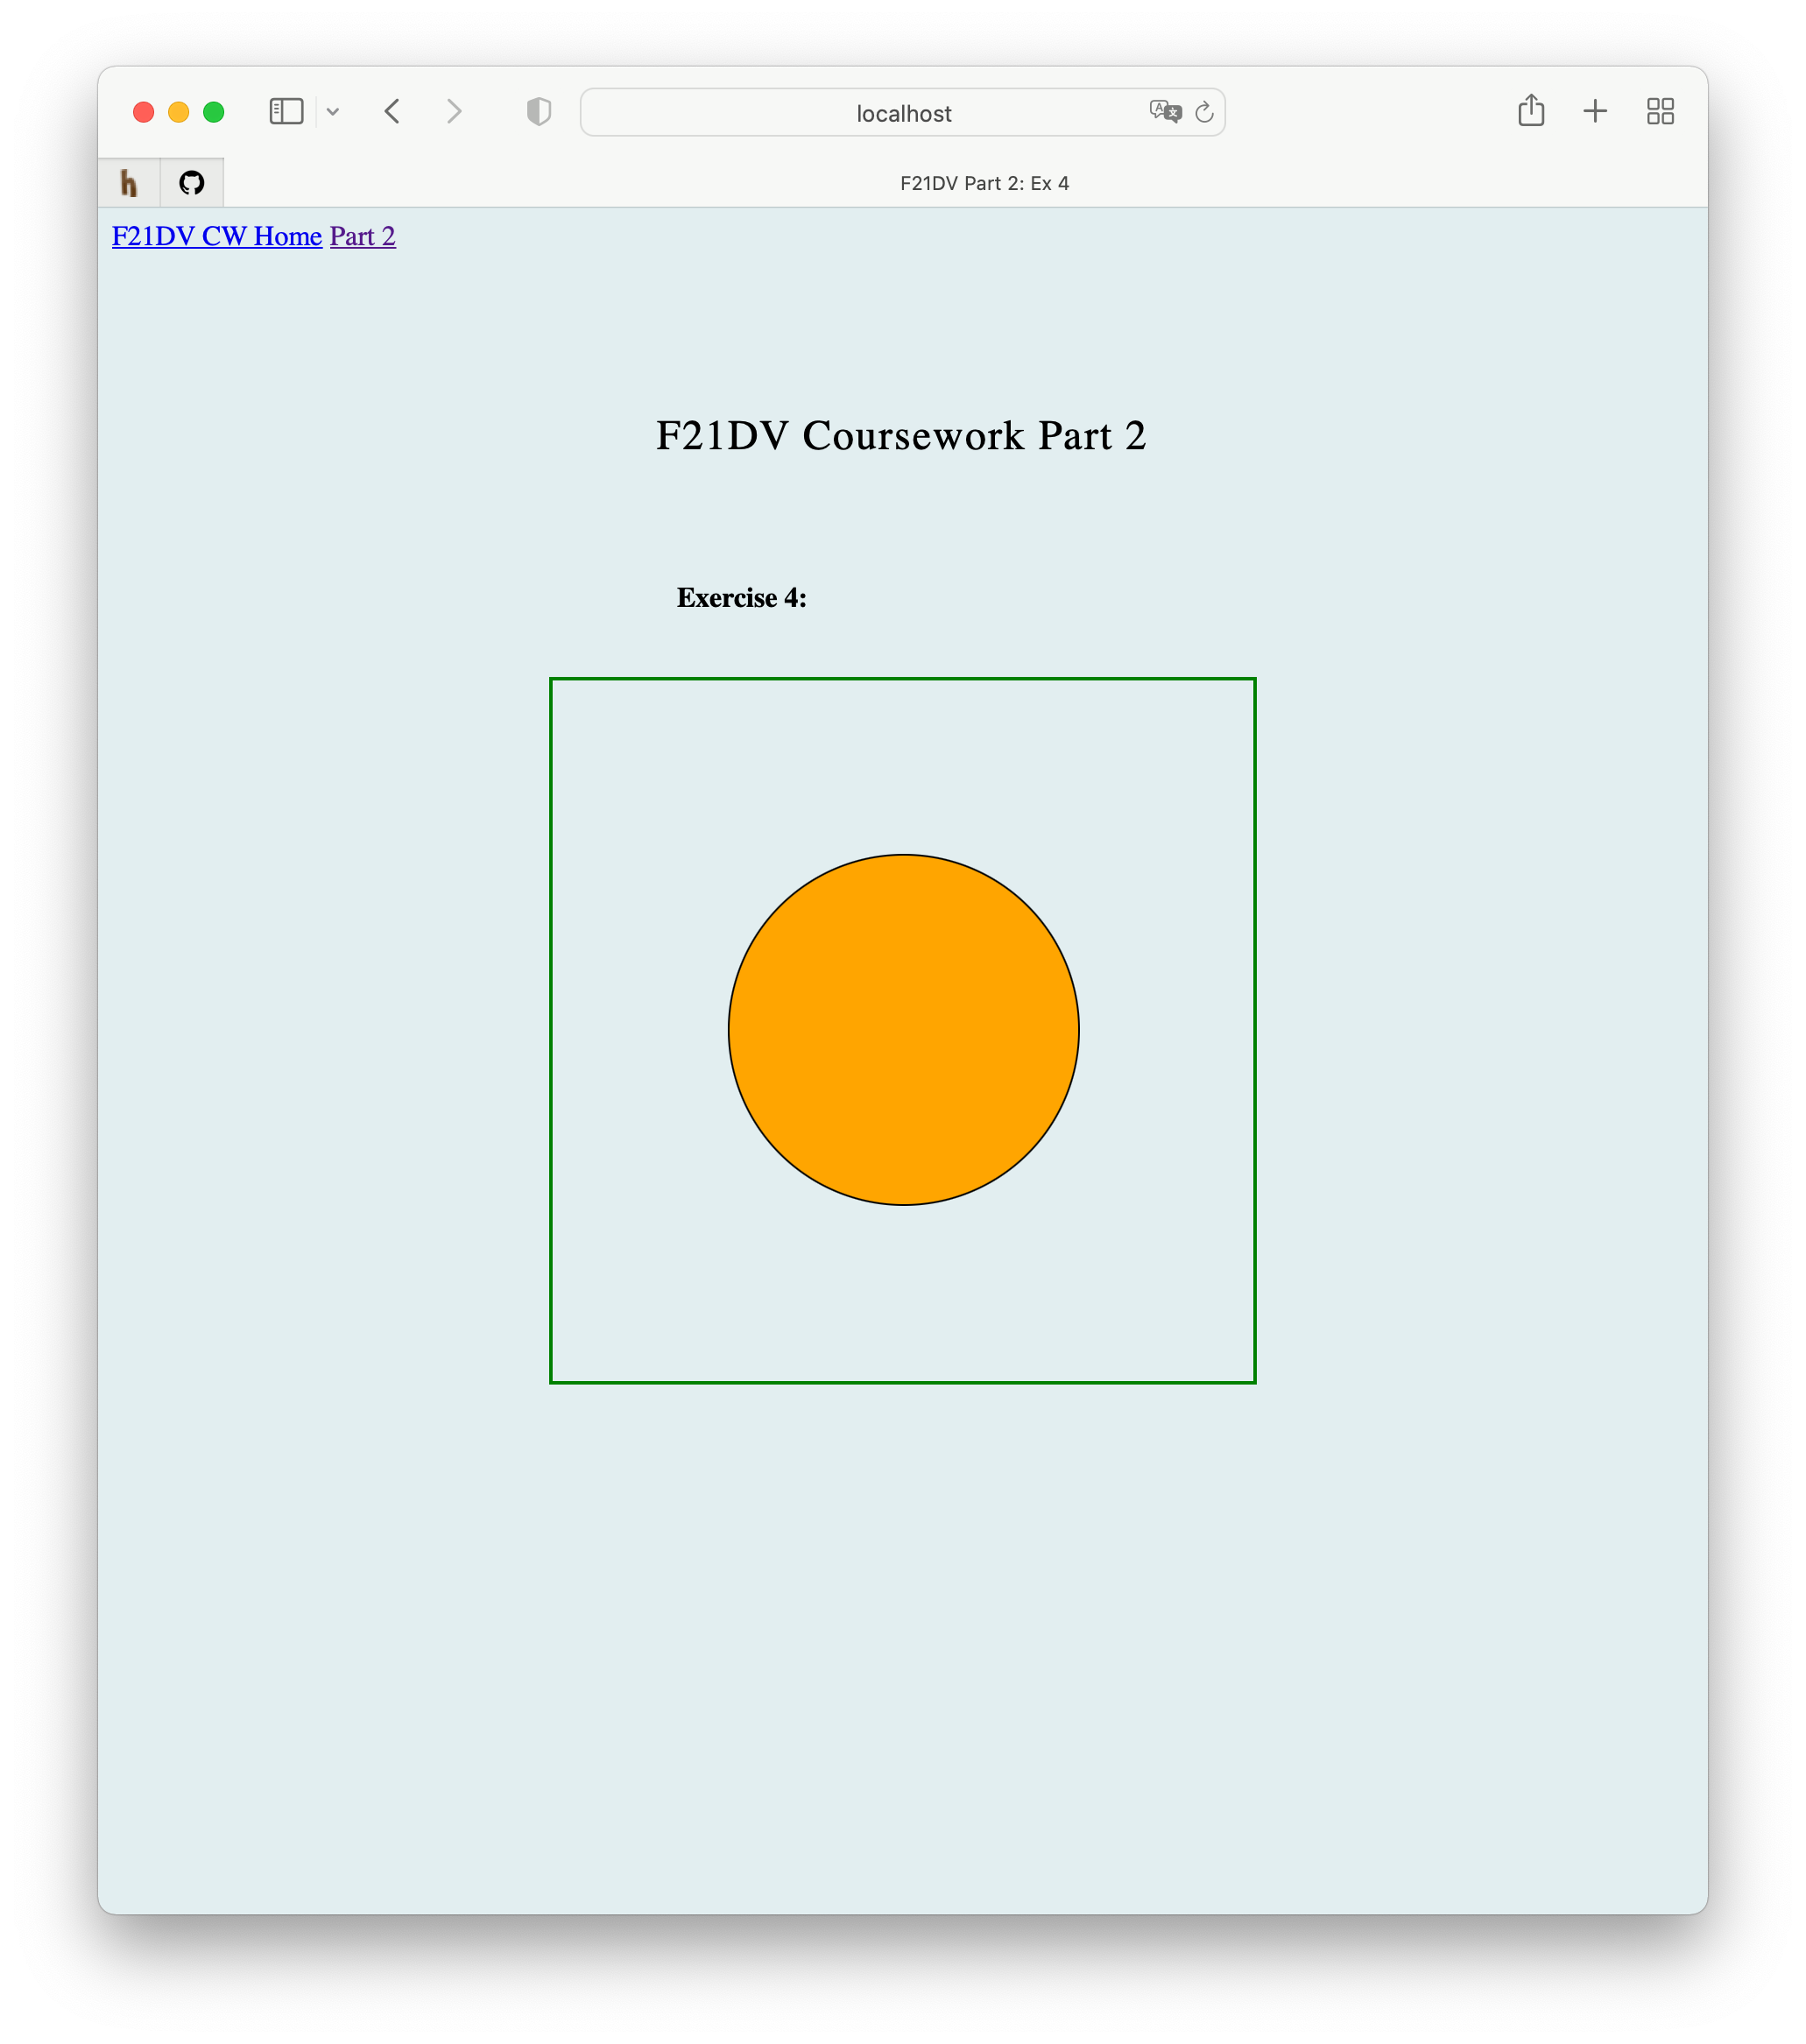
\includegraphics[width = 7.5cm]{images/ex4_1.png}
    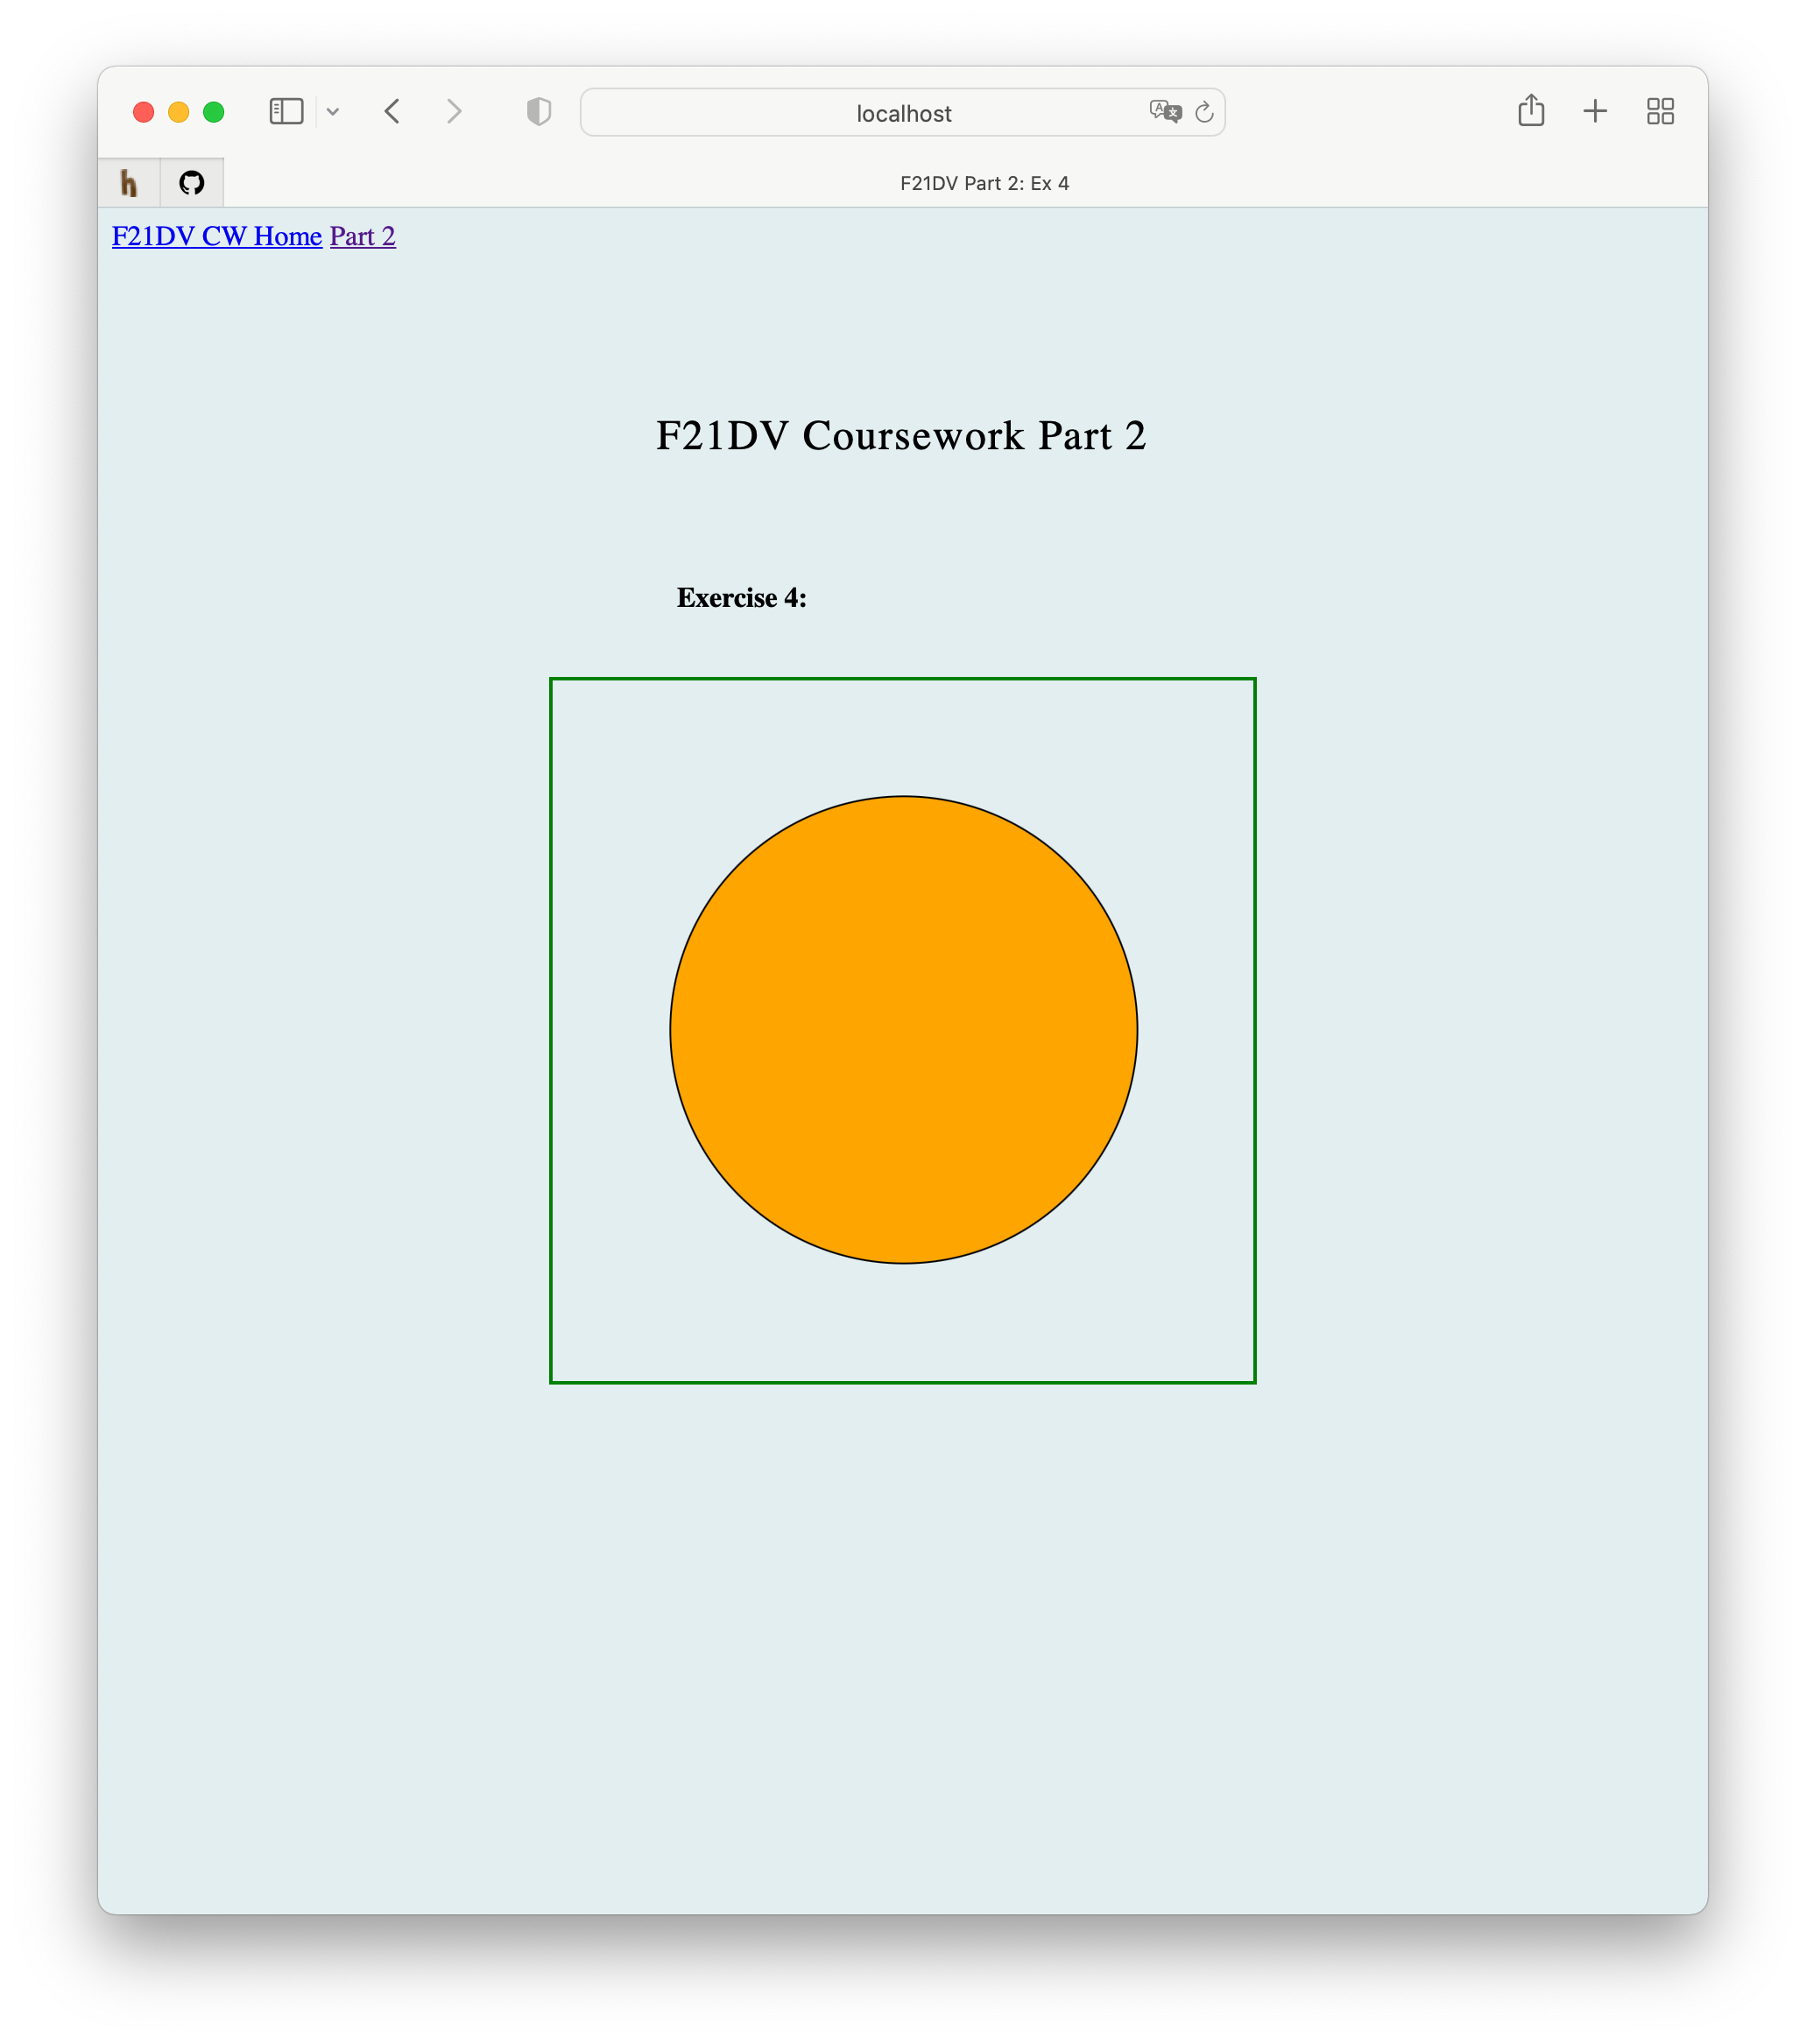
\includegraphics[width = 7.5cm]{images/ex4_2.png}
    \label{fig:ex4}
    \caption{Exercise 4}
\end{figure}
\FloatBarrier
% \lstinputlisting[language=JavaScript]{../../public/js/part2/task4.js}
Figure \ref{fig:ex4} shows an SVG object with a circle in the middle. Upon hovering on the circle, the circle enlarges. This time, the action was modeled using d3 transitions instead of css :hover method. I've added transtitions upon mouse hover and out.
\section{Exercise 10}
Exactly the same as exercise 4, just that the ease method has been changed to \verb|d3.easeBounce|.

\newpage
\section{Exercise 5}
\begin{figure}[!ht]
    \centering
    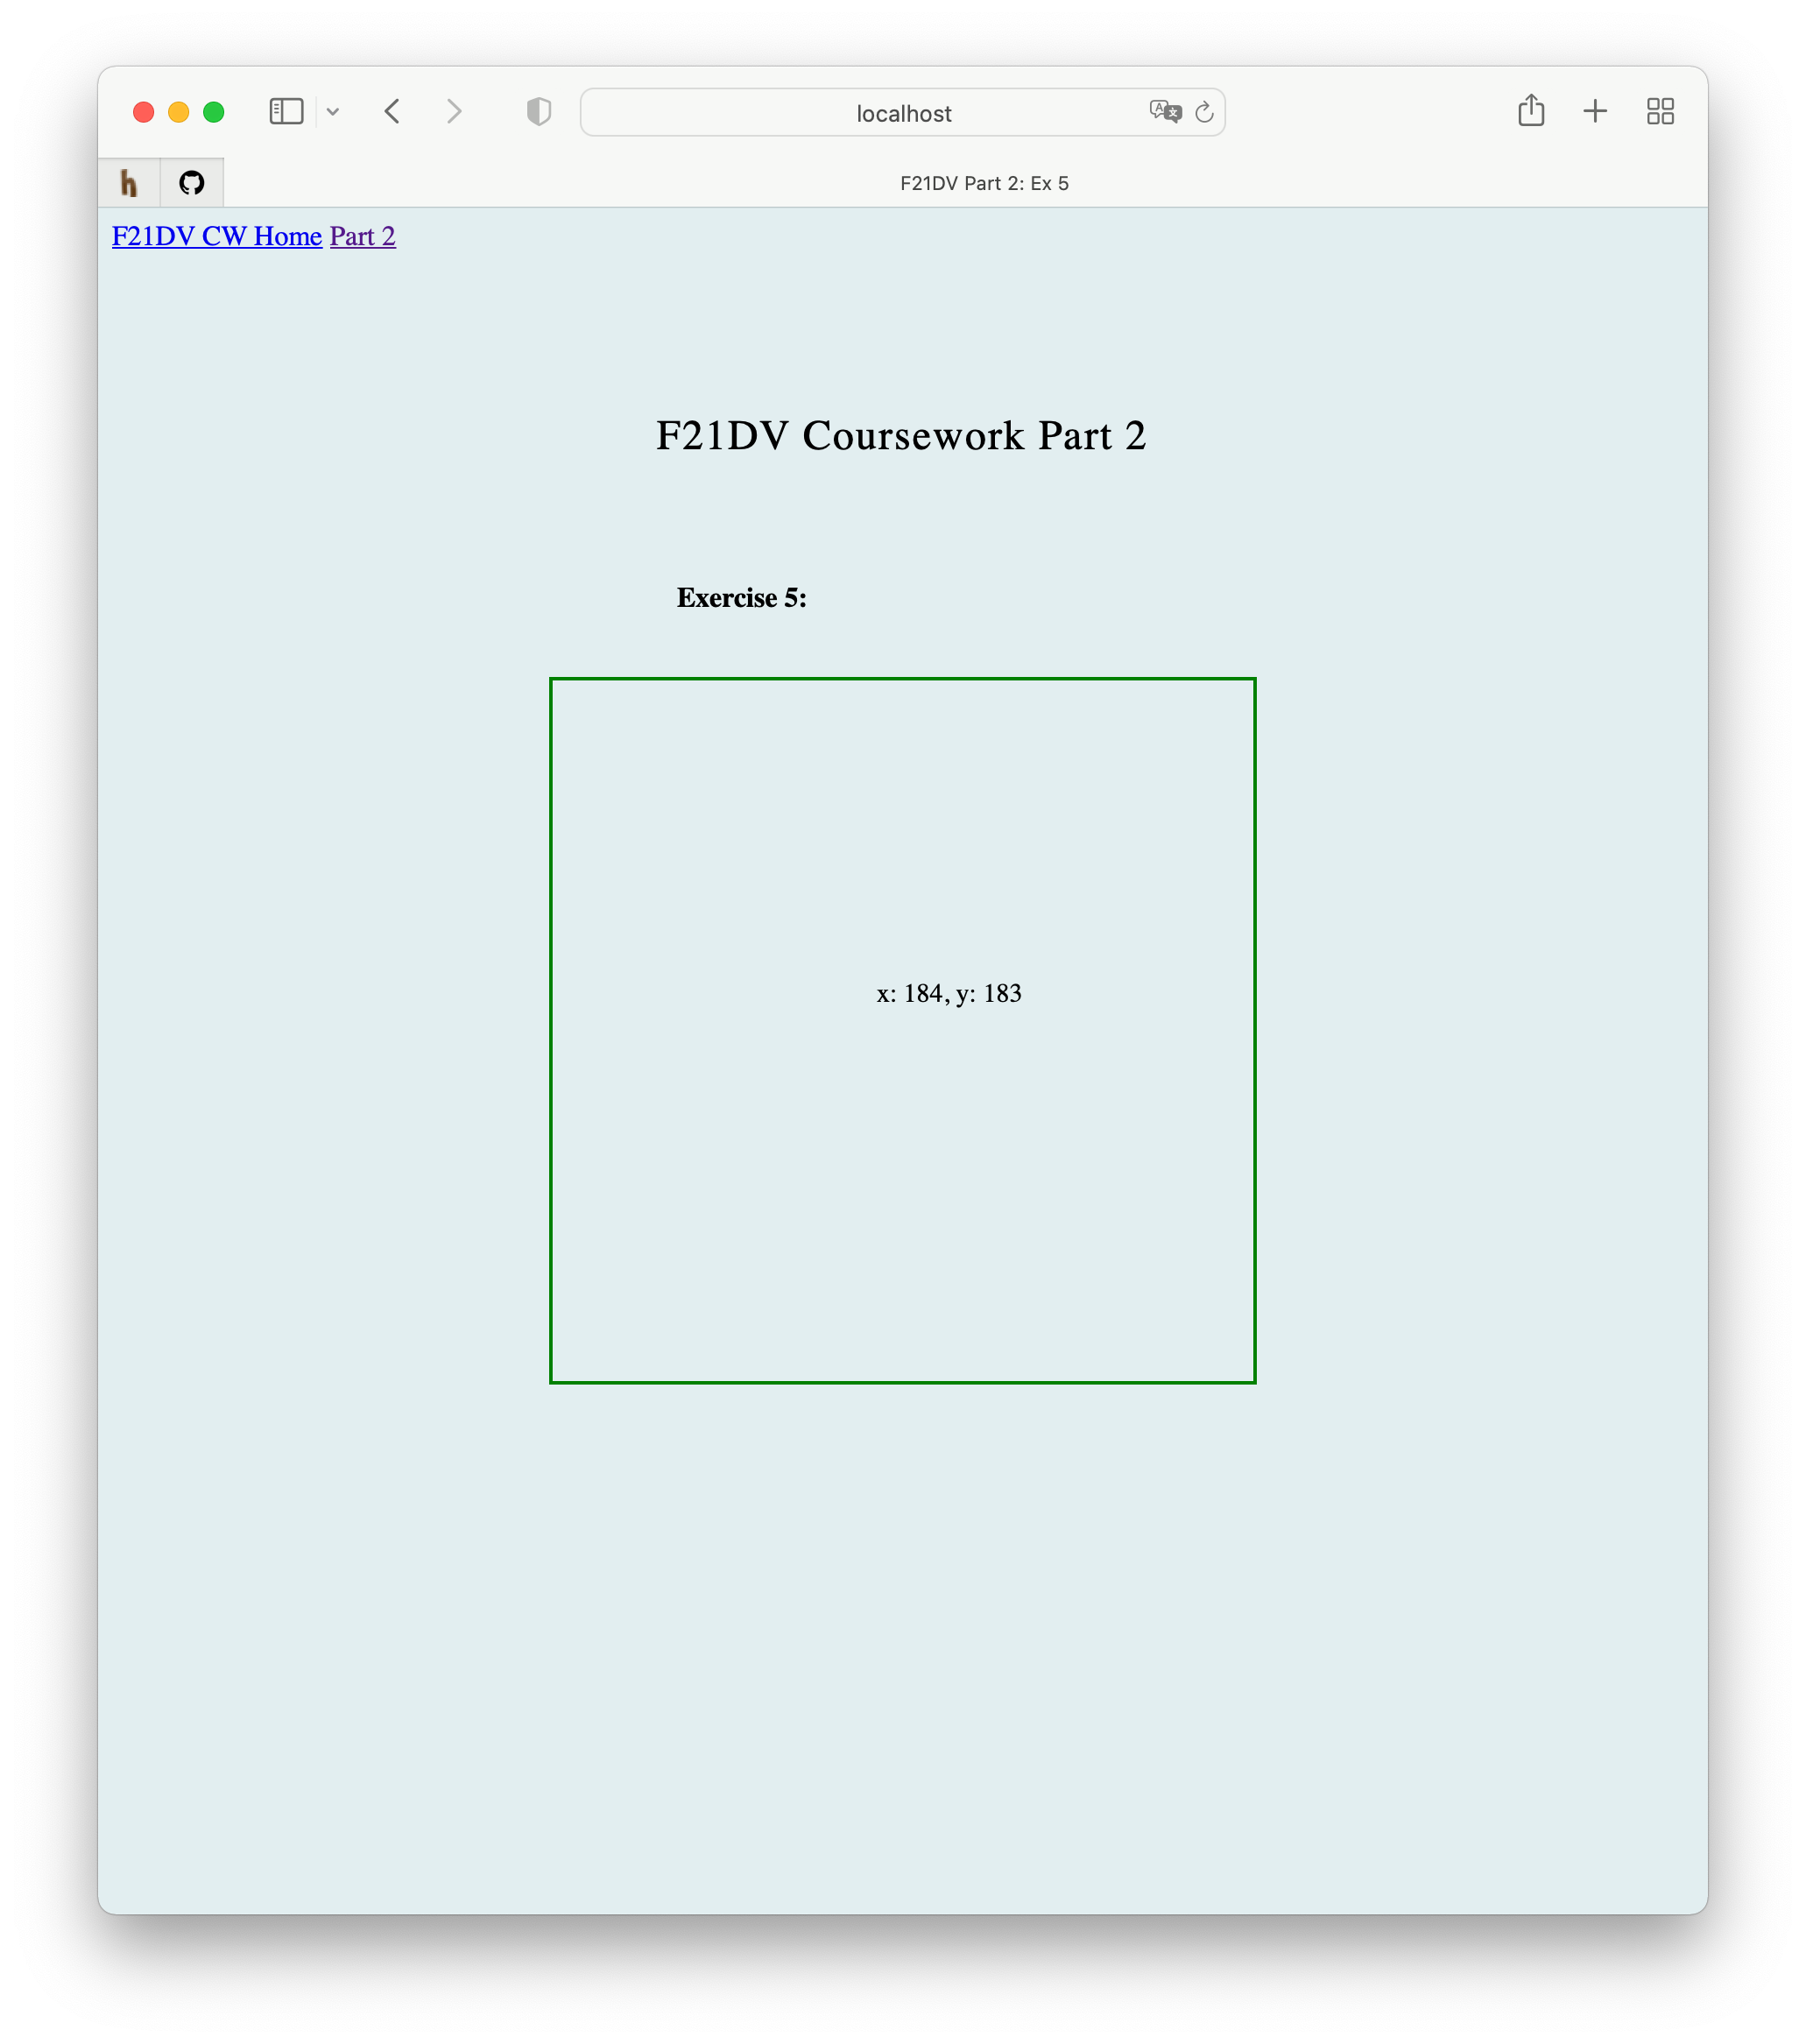
\includegraphics[width = 7.5cm]{images/ex5.png}
    % 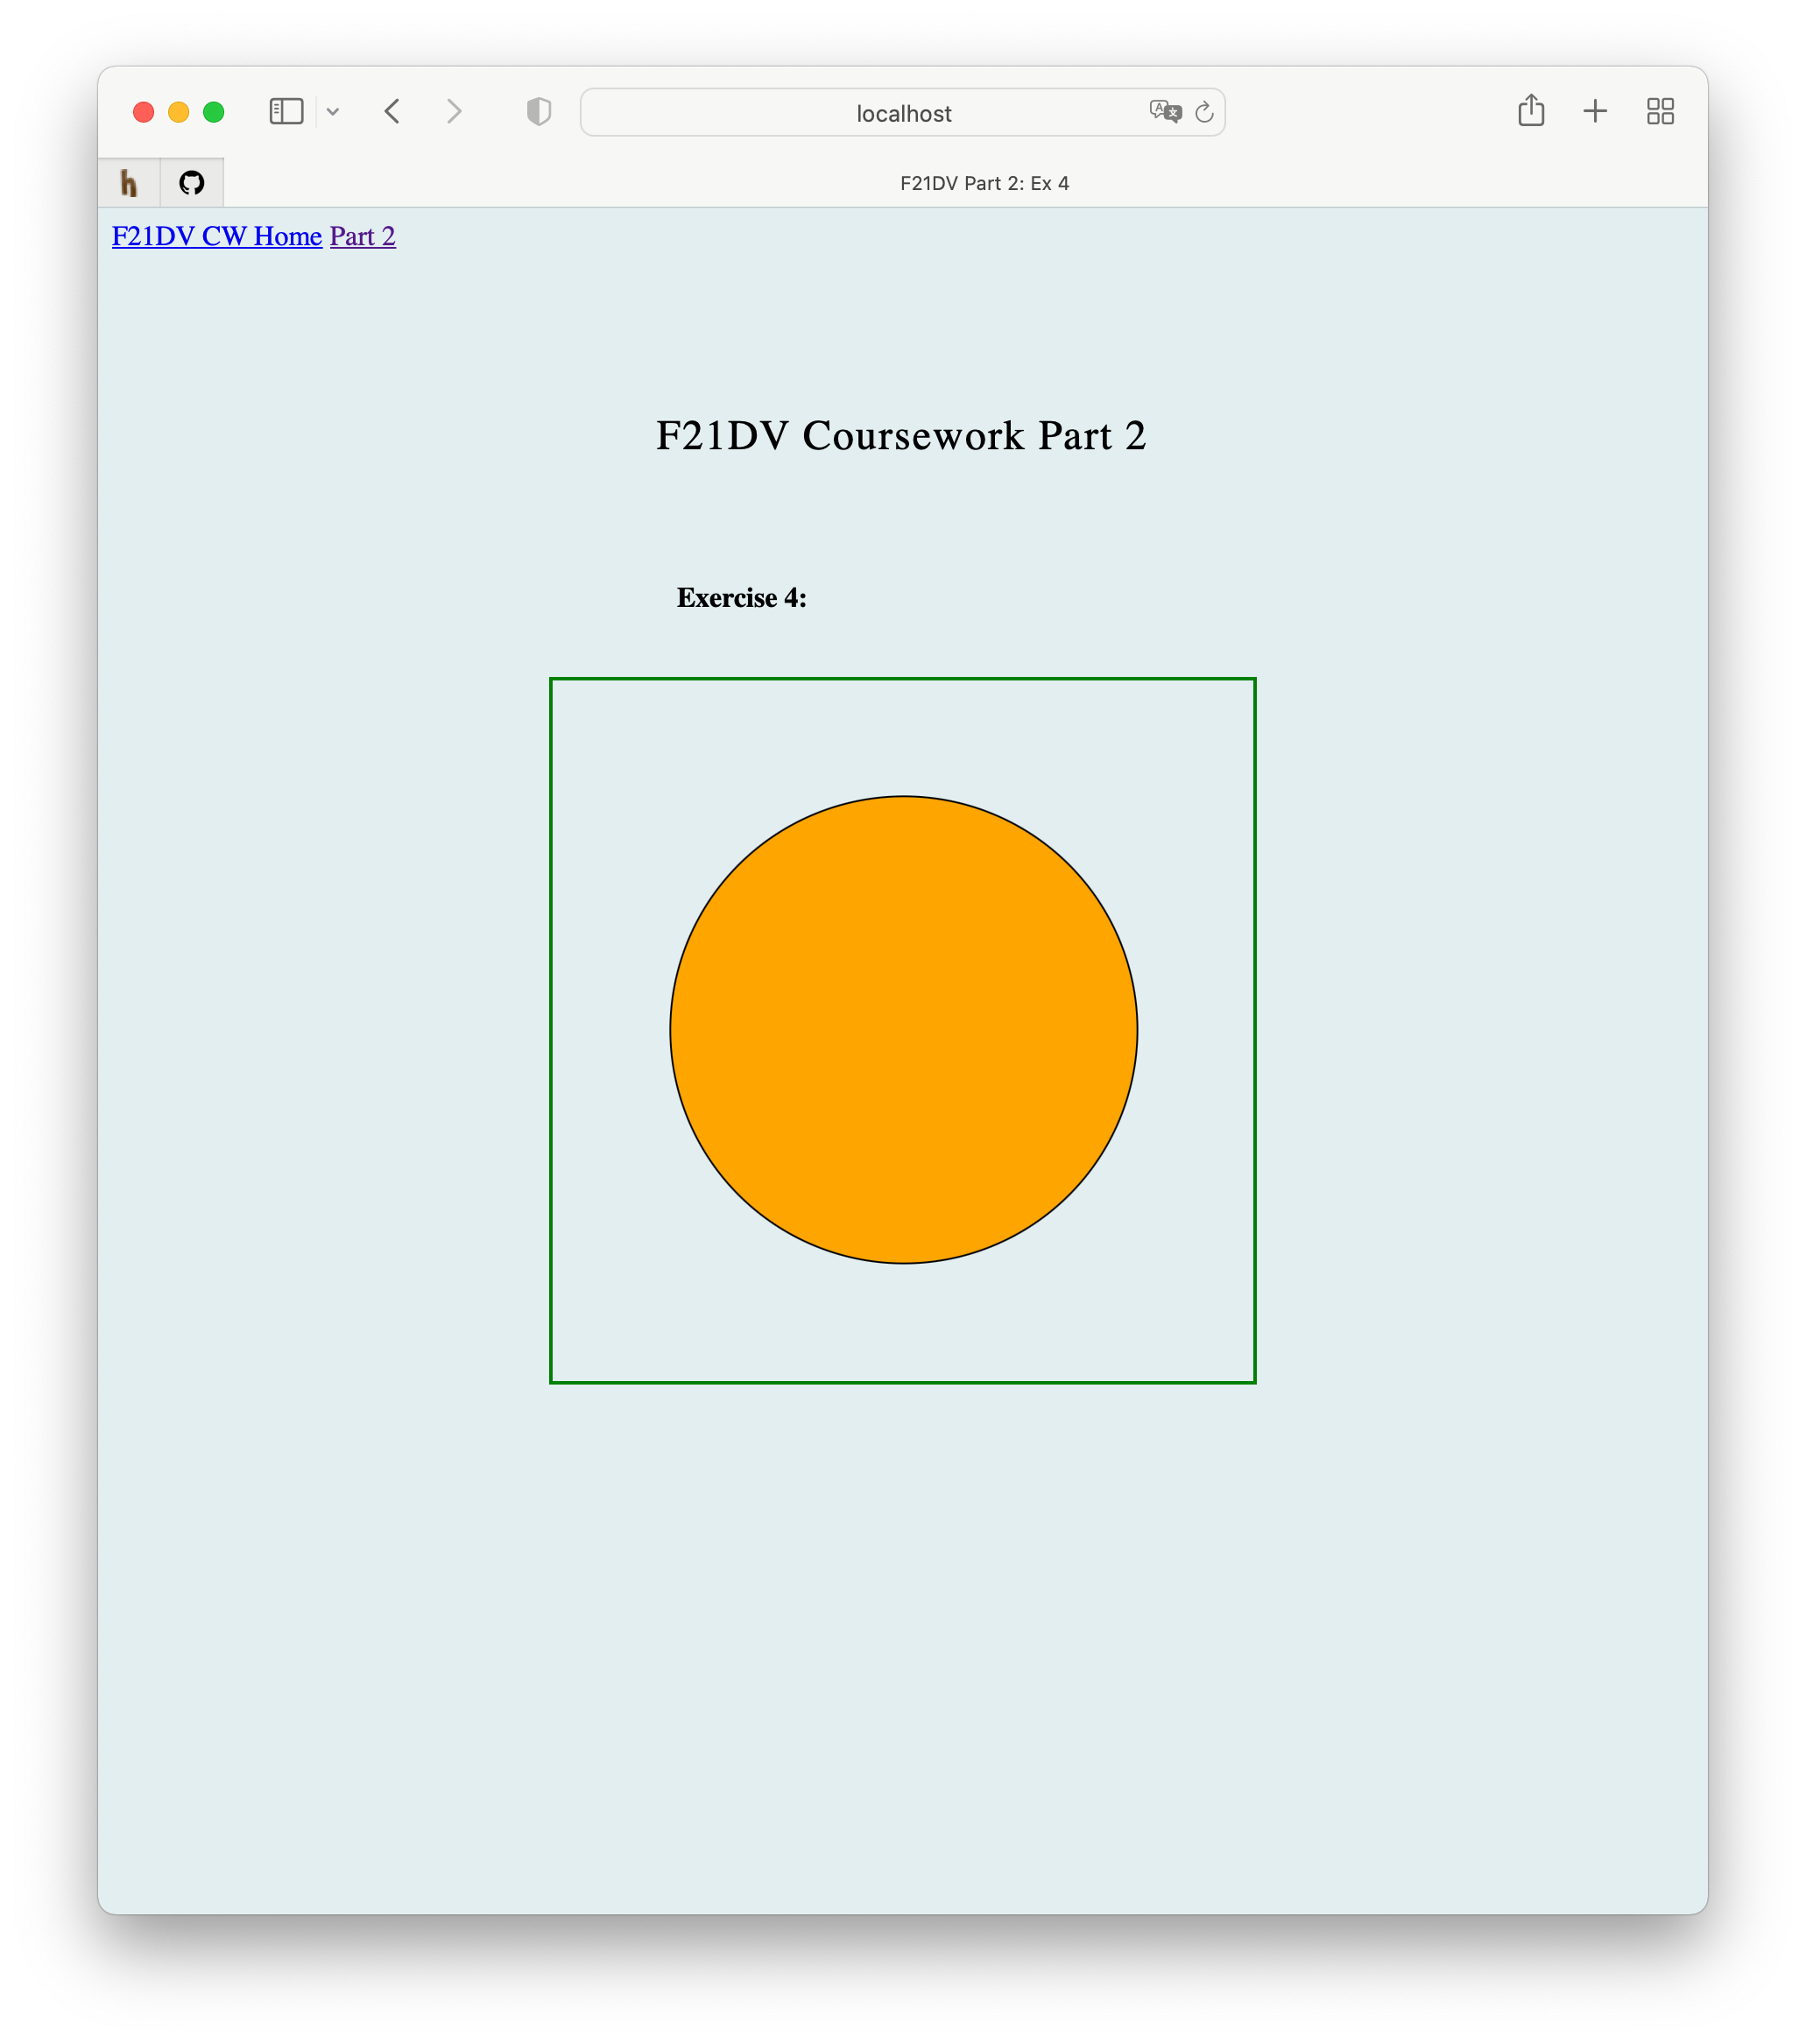
\includegraphics[width = 7.5cm]{images/ex4_2.png}
    \label{fig:ex5}
    \caption{Exercise 5}
\end{figure}
\FloatBarrier
% \lstinputlisting[language=JavaScript]{../../public/js/part2/task5.js}
Figure \ref{fig:ex5} shows an emptey svg object, and upon mouse hover, it would show the corredinated of the mouse. There was also a pre-appended empty text box. To show the x-y coordinates, this is done using the event data of the mouse movement. Then using the data, I modified the `x' and `y' attribute of the text box.

\newpage
\section{Exercise 6}
\begin{figure}[!ht]
    \centering
    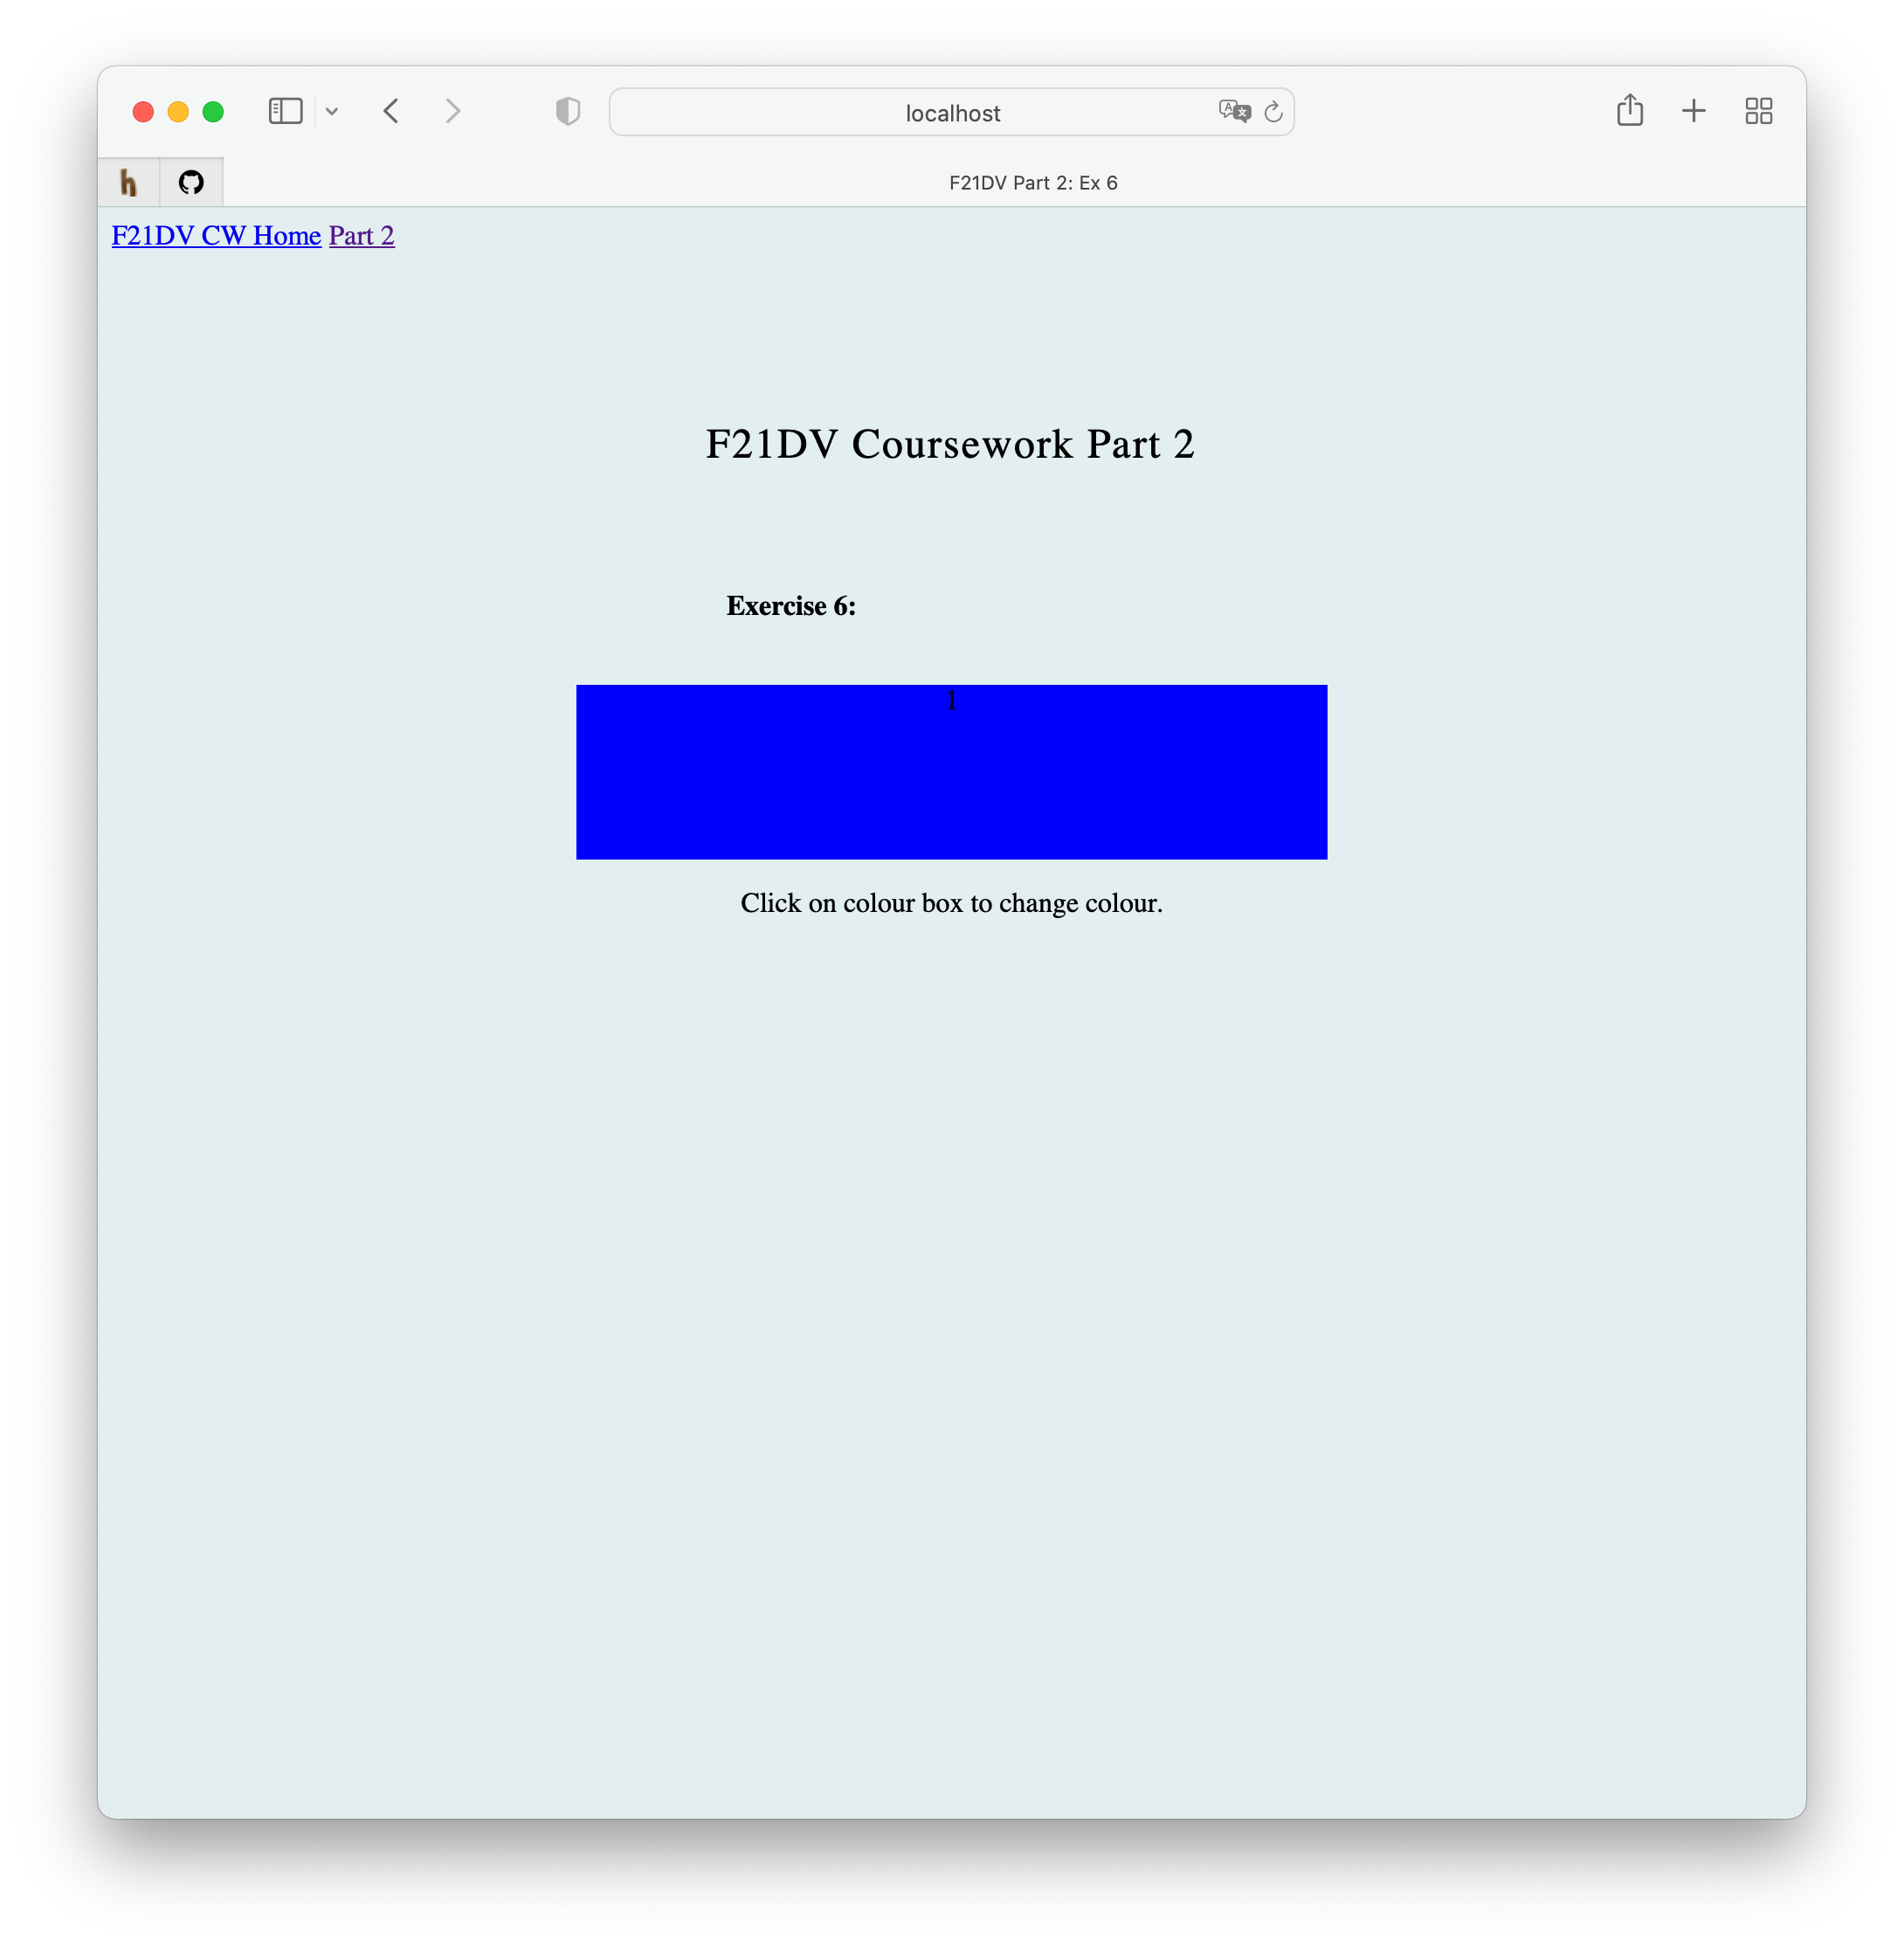
\includegraphics[width = 7.5cm]{images/ex6_1.png}
    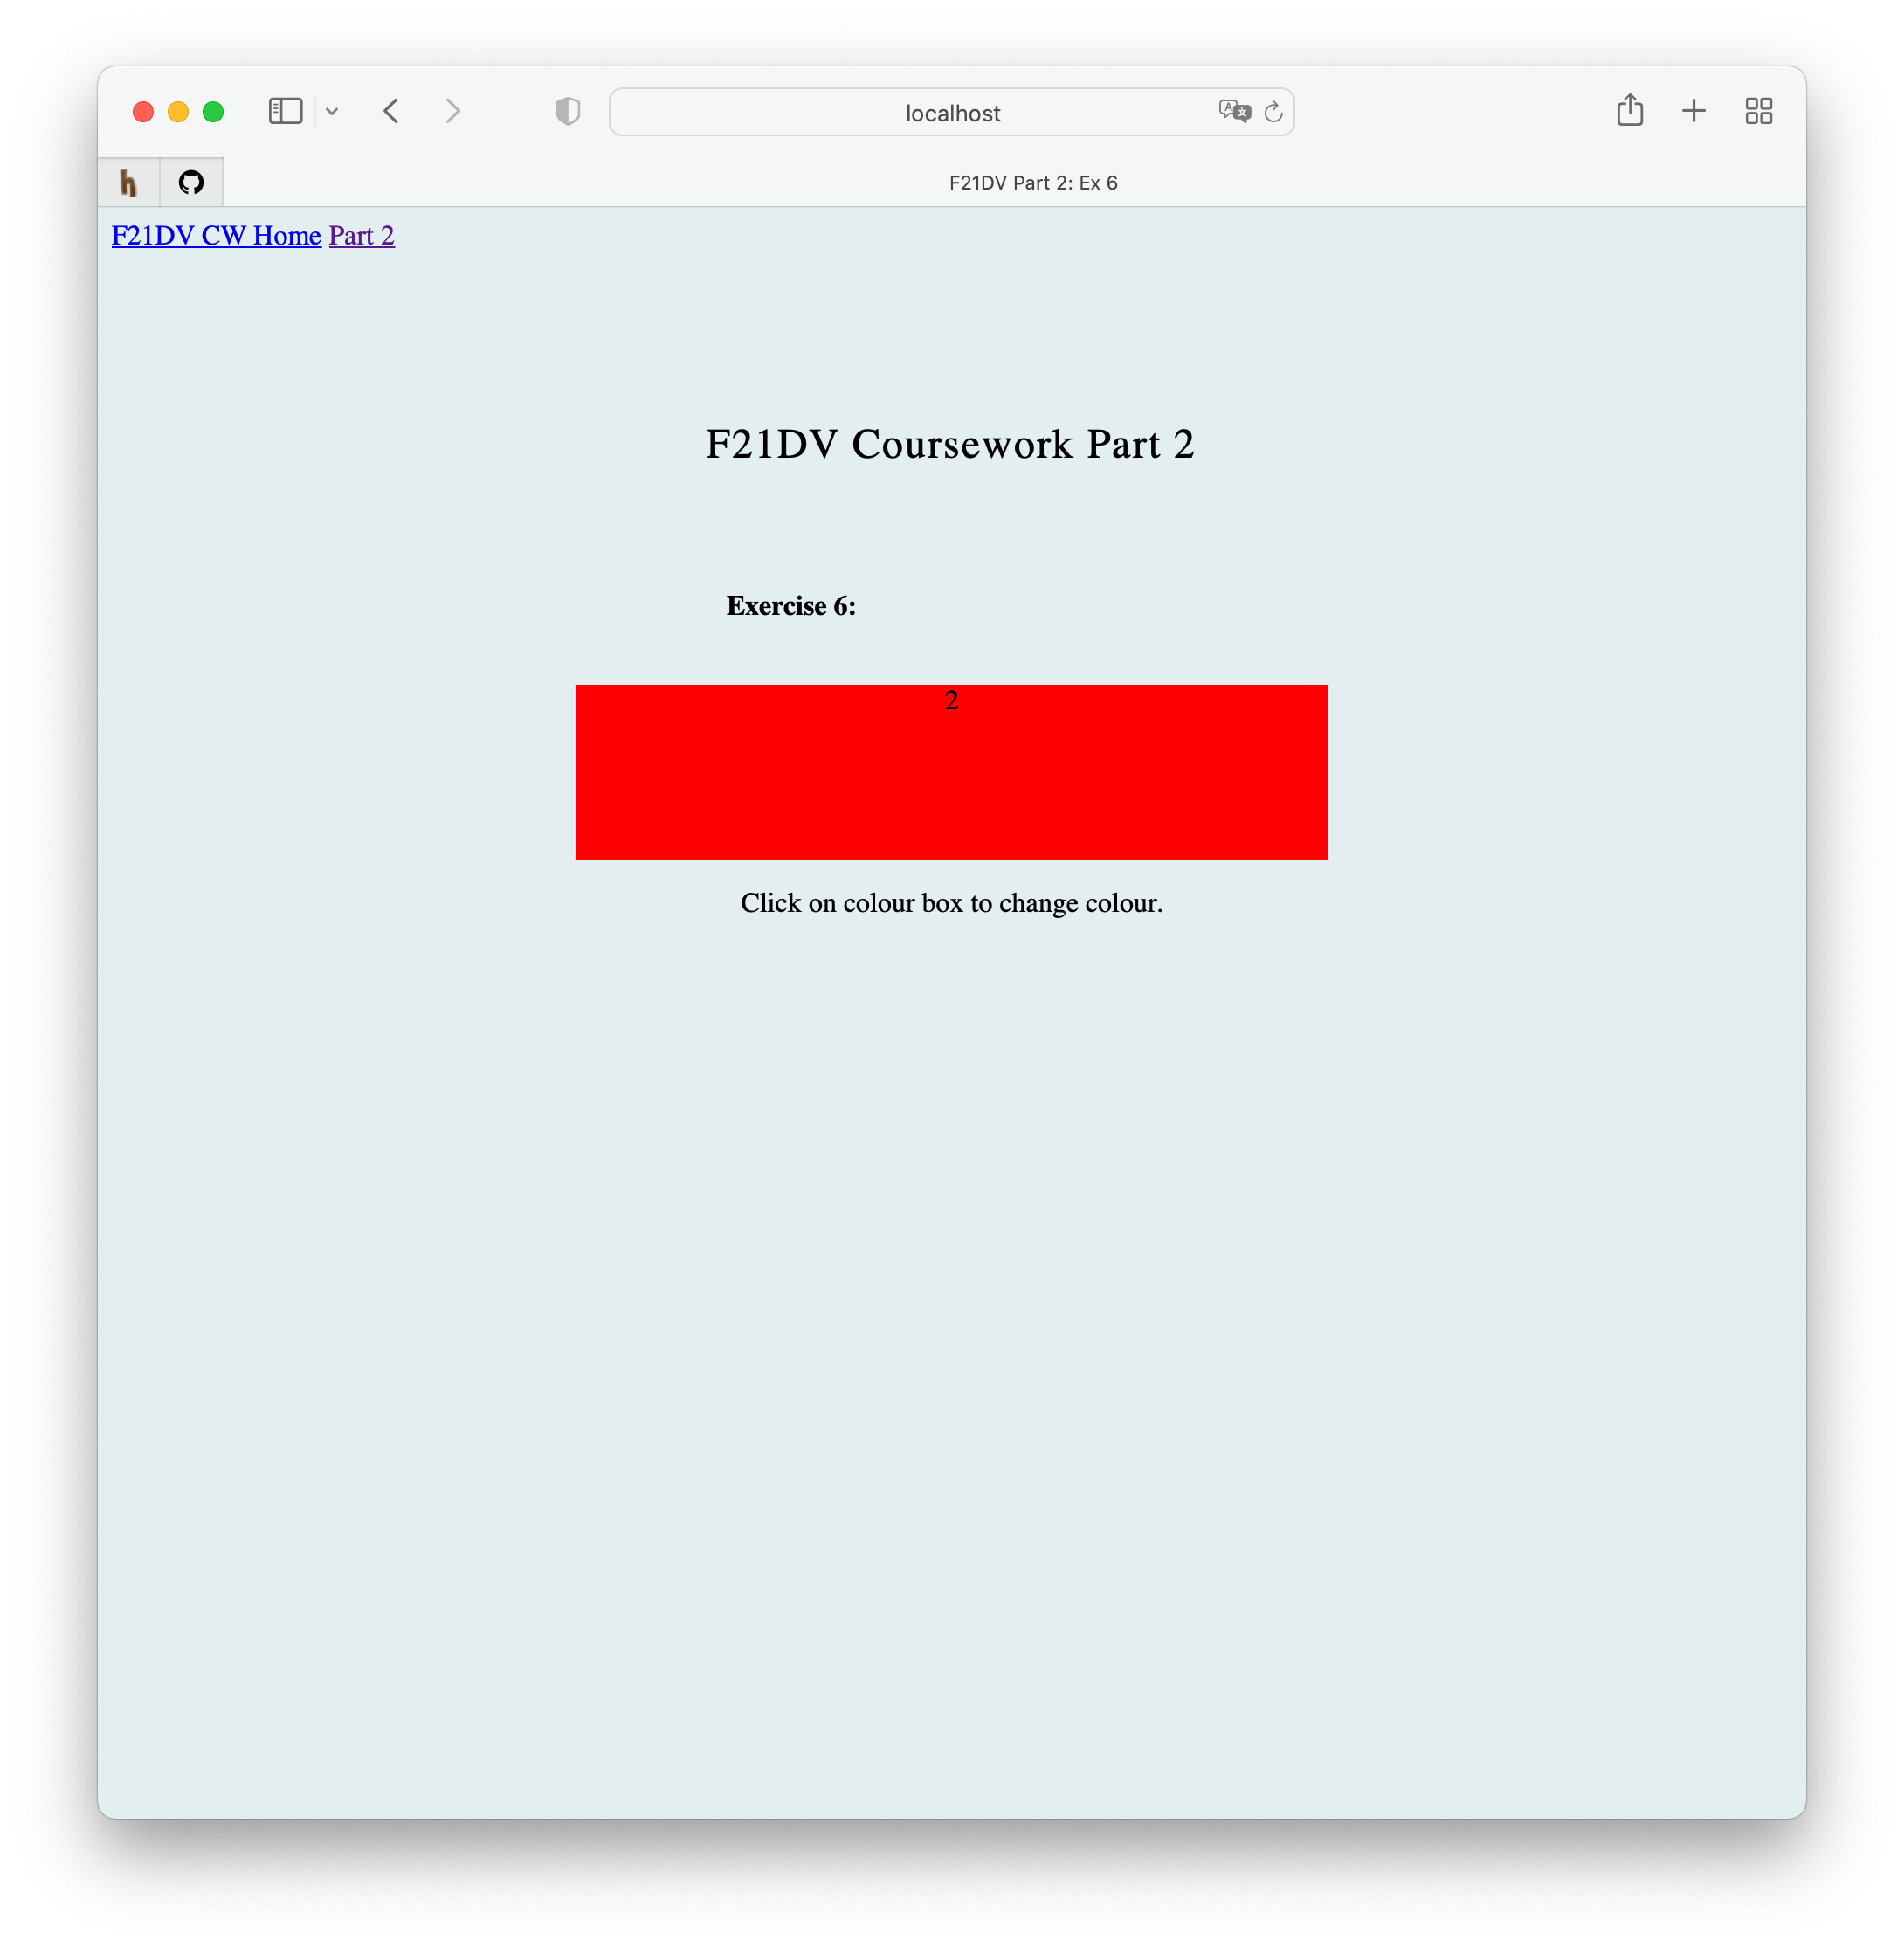
\includegraphics[width = 7.5cm]{images/ex6_2.png}
    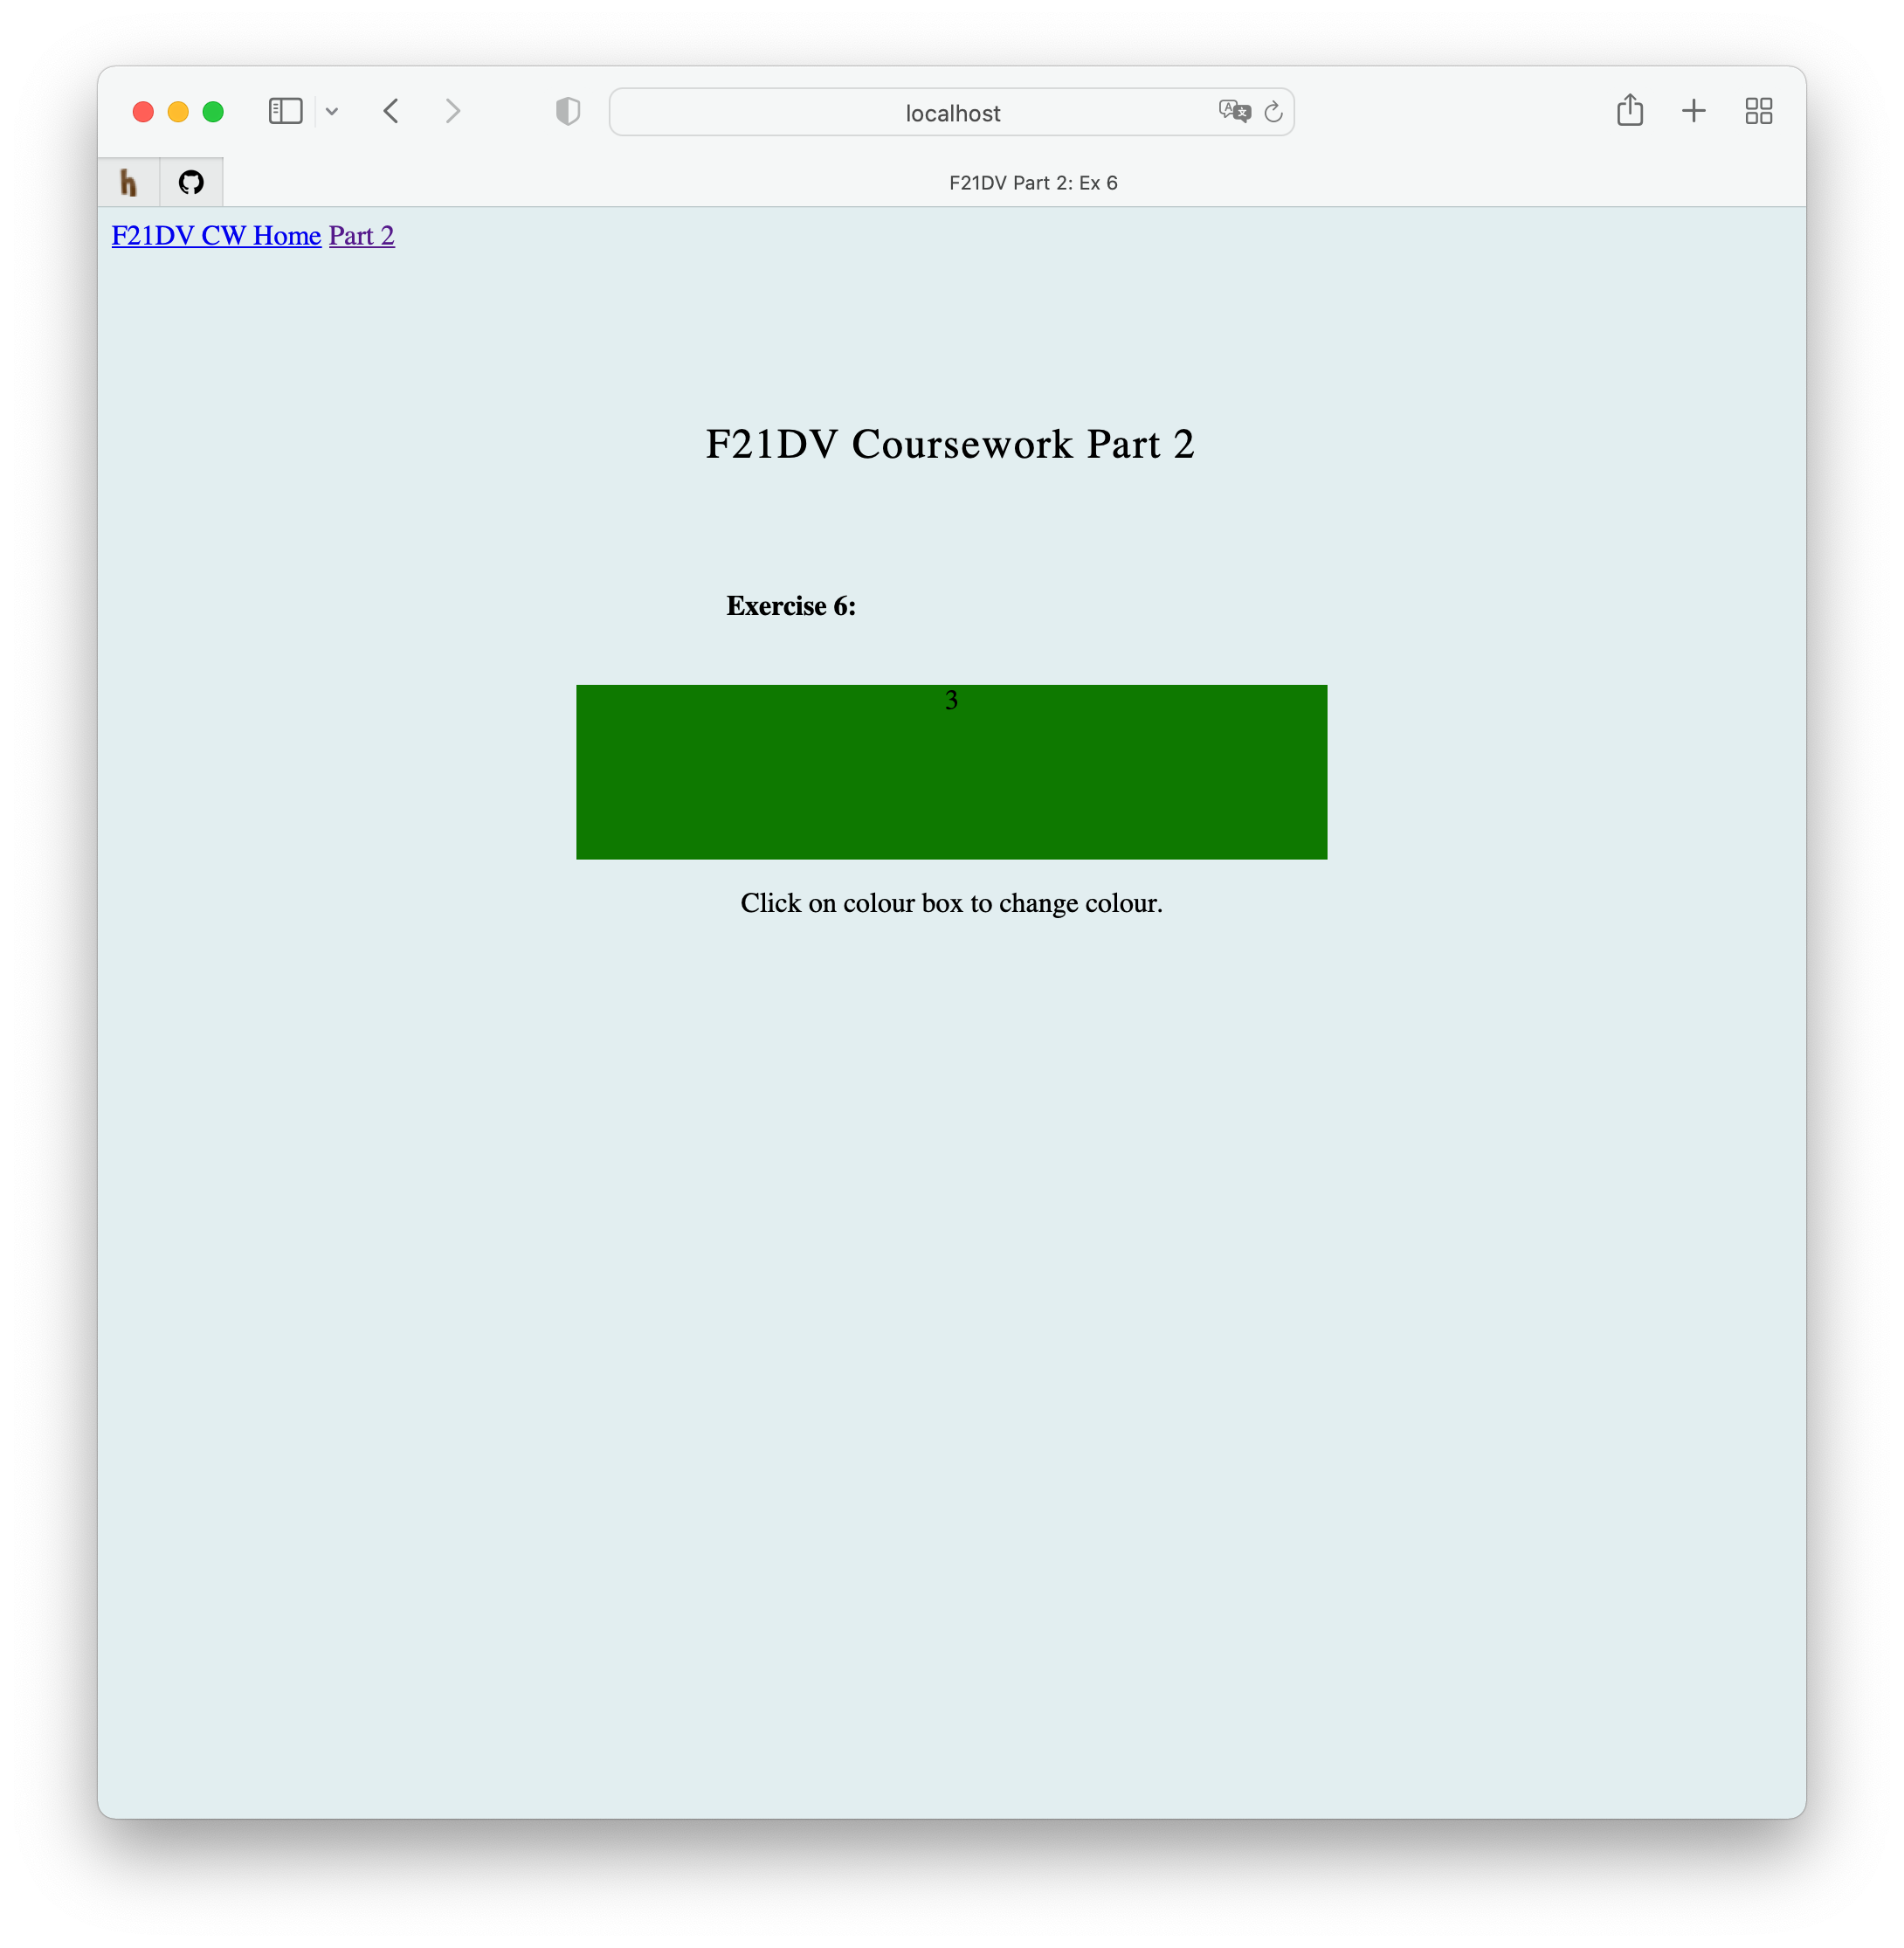
\includegraphics[width = 7.5cm]{images/ex6_3.png}
    \label{fig:ex6}
    \caption{Exercise 6}
\end{figure}
\FloatBarrier
\lstinputlisting[language=JavaScript]{../../public/js/part2/task6.js}
Figure \ref{fig:ex6} shows a coloured div with a number on it. On click, this div will transition to ``2'' and change to red, and then to ``3'' and then to green. Finally it will transition back to the original form. From listing above, we could see that this is done by using the transition upon mouse click, then changing the attributes of the div.

\newpage
\section{Exercise 7}
\begin{figure}[!ht]
    \centering
    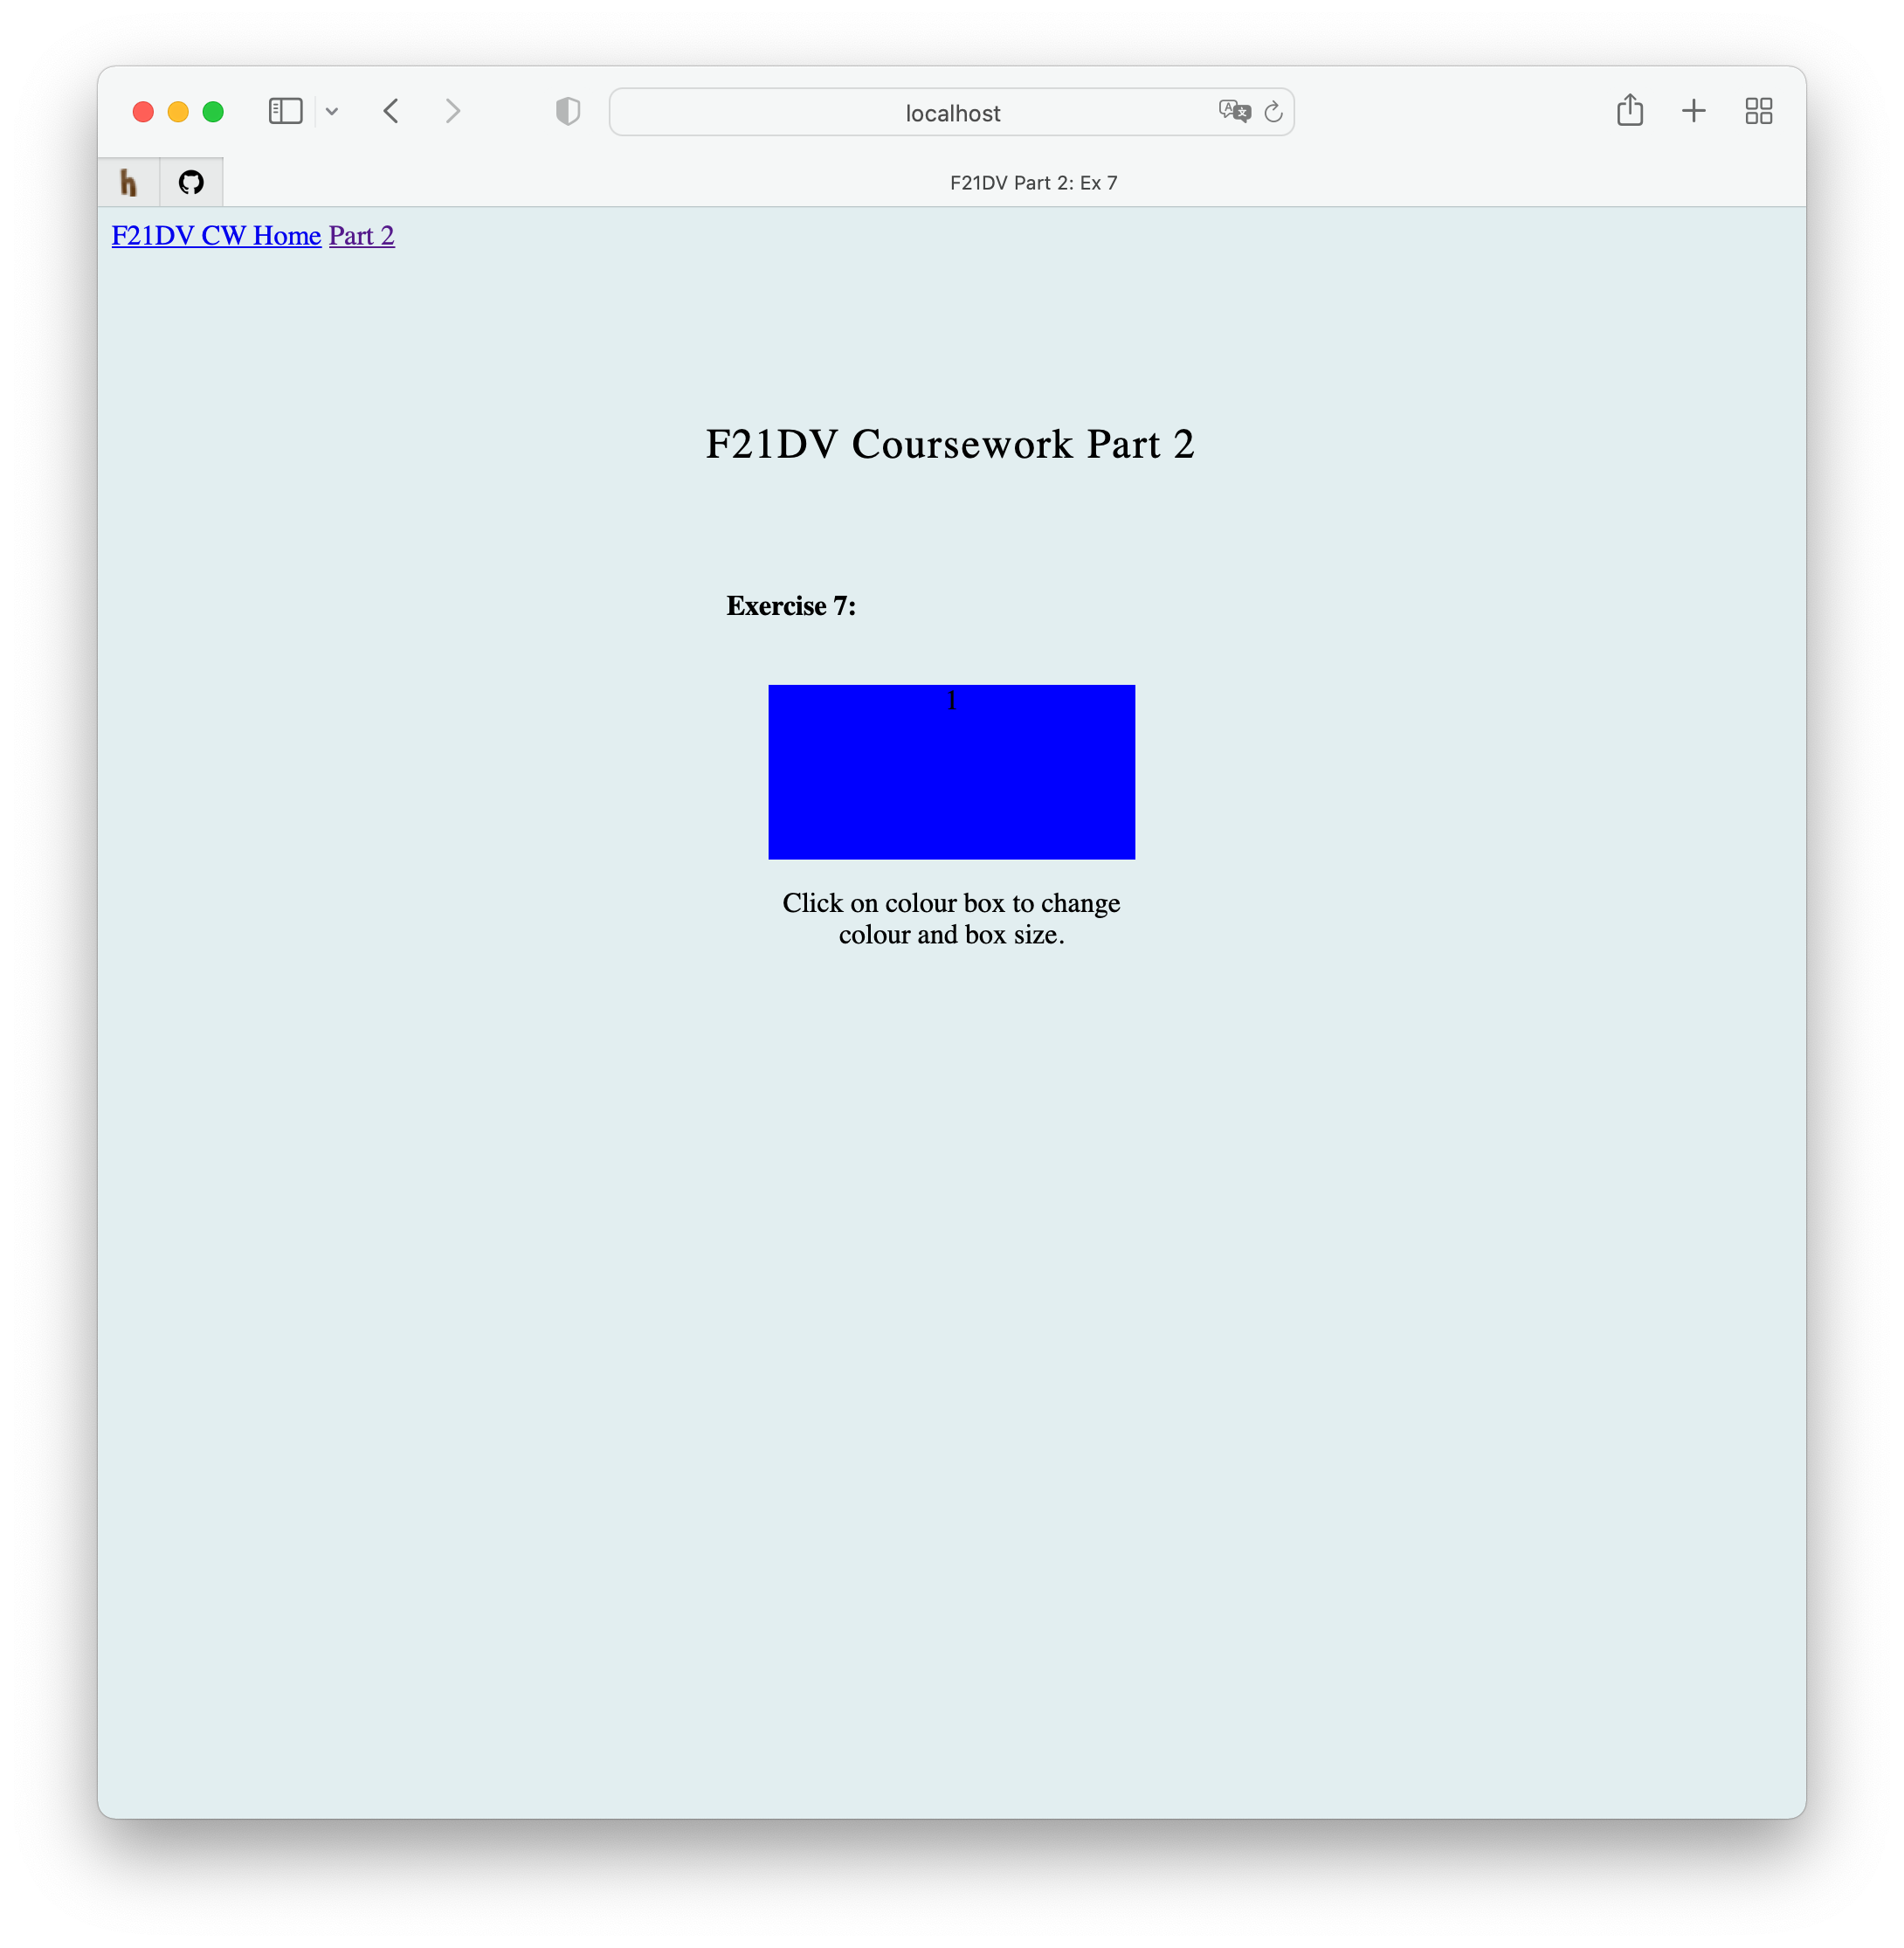
\includegraphics[width = 7.5cm]{images/ex7_1.png}
    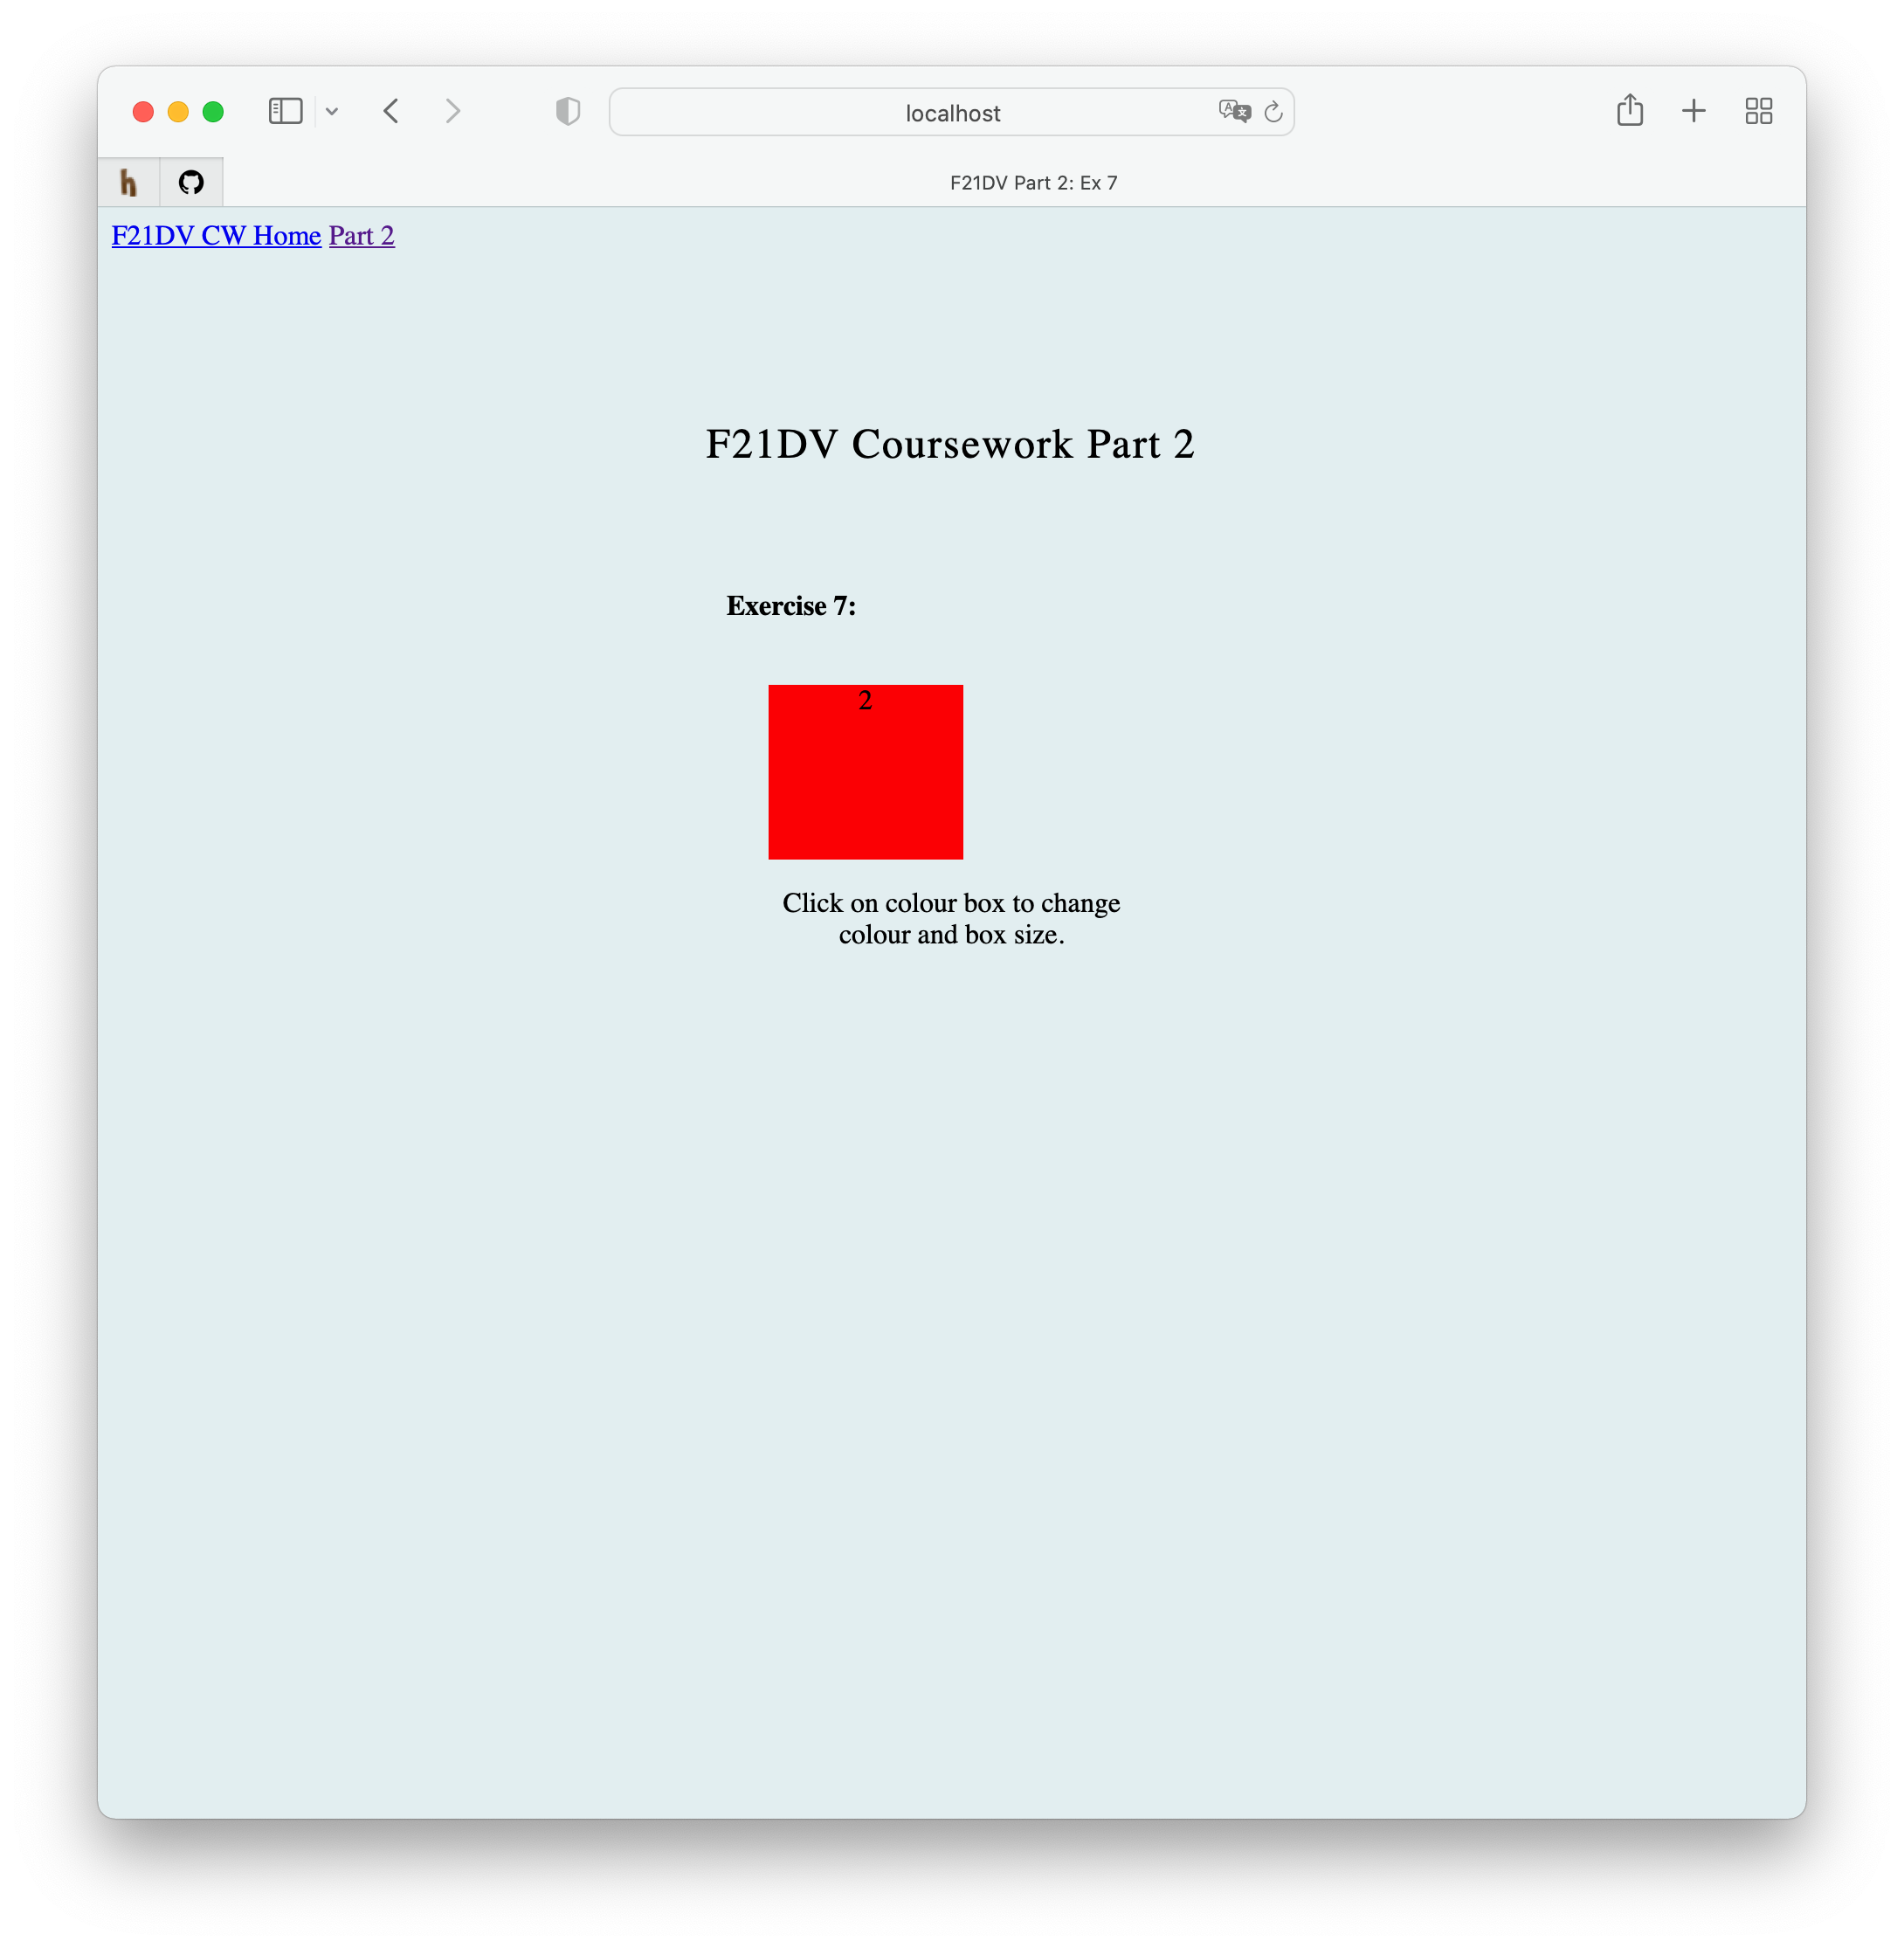
\includegraphics[width = 7.5cm]{images/ex7_2.png}
    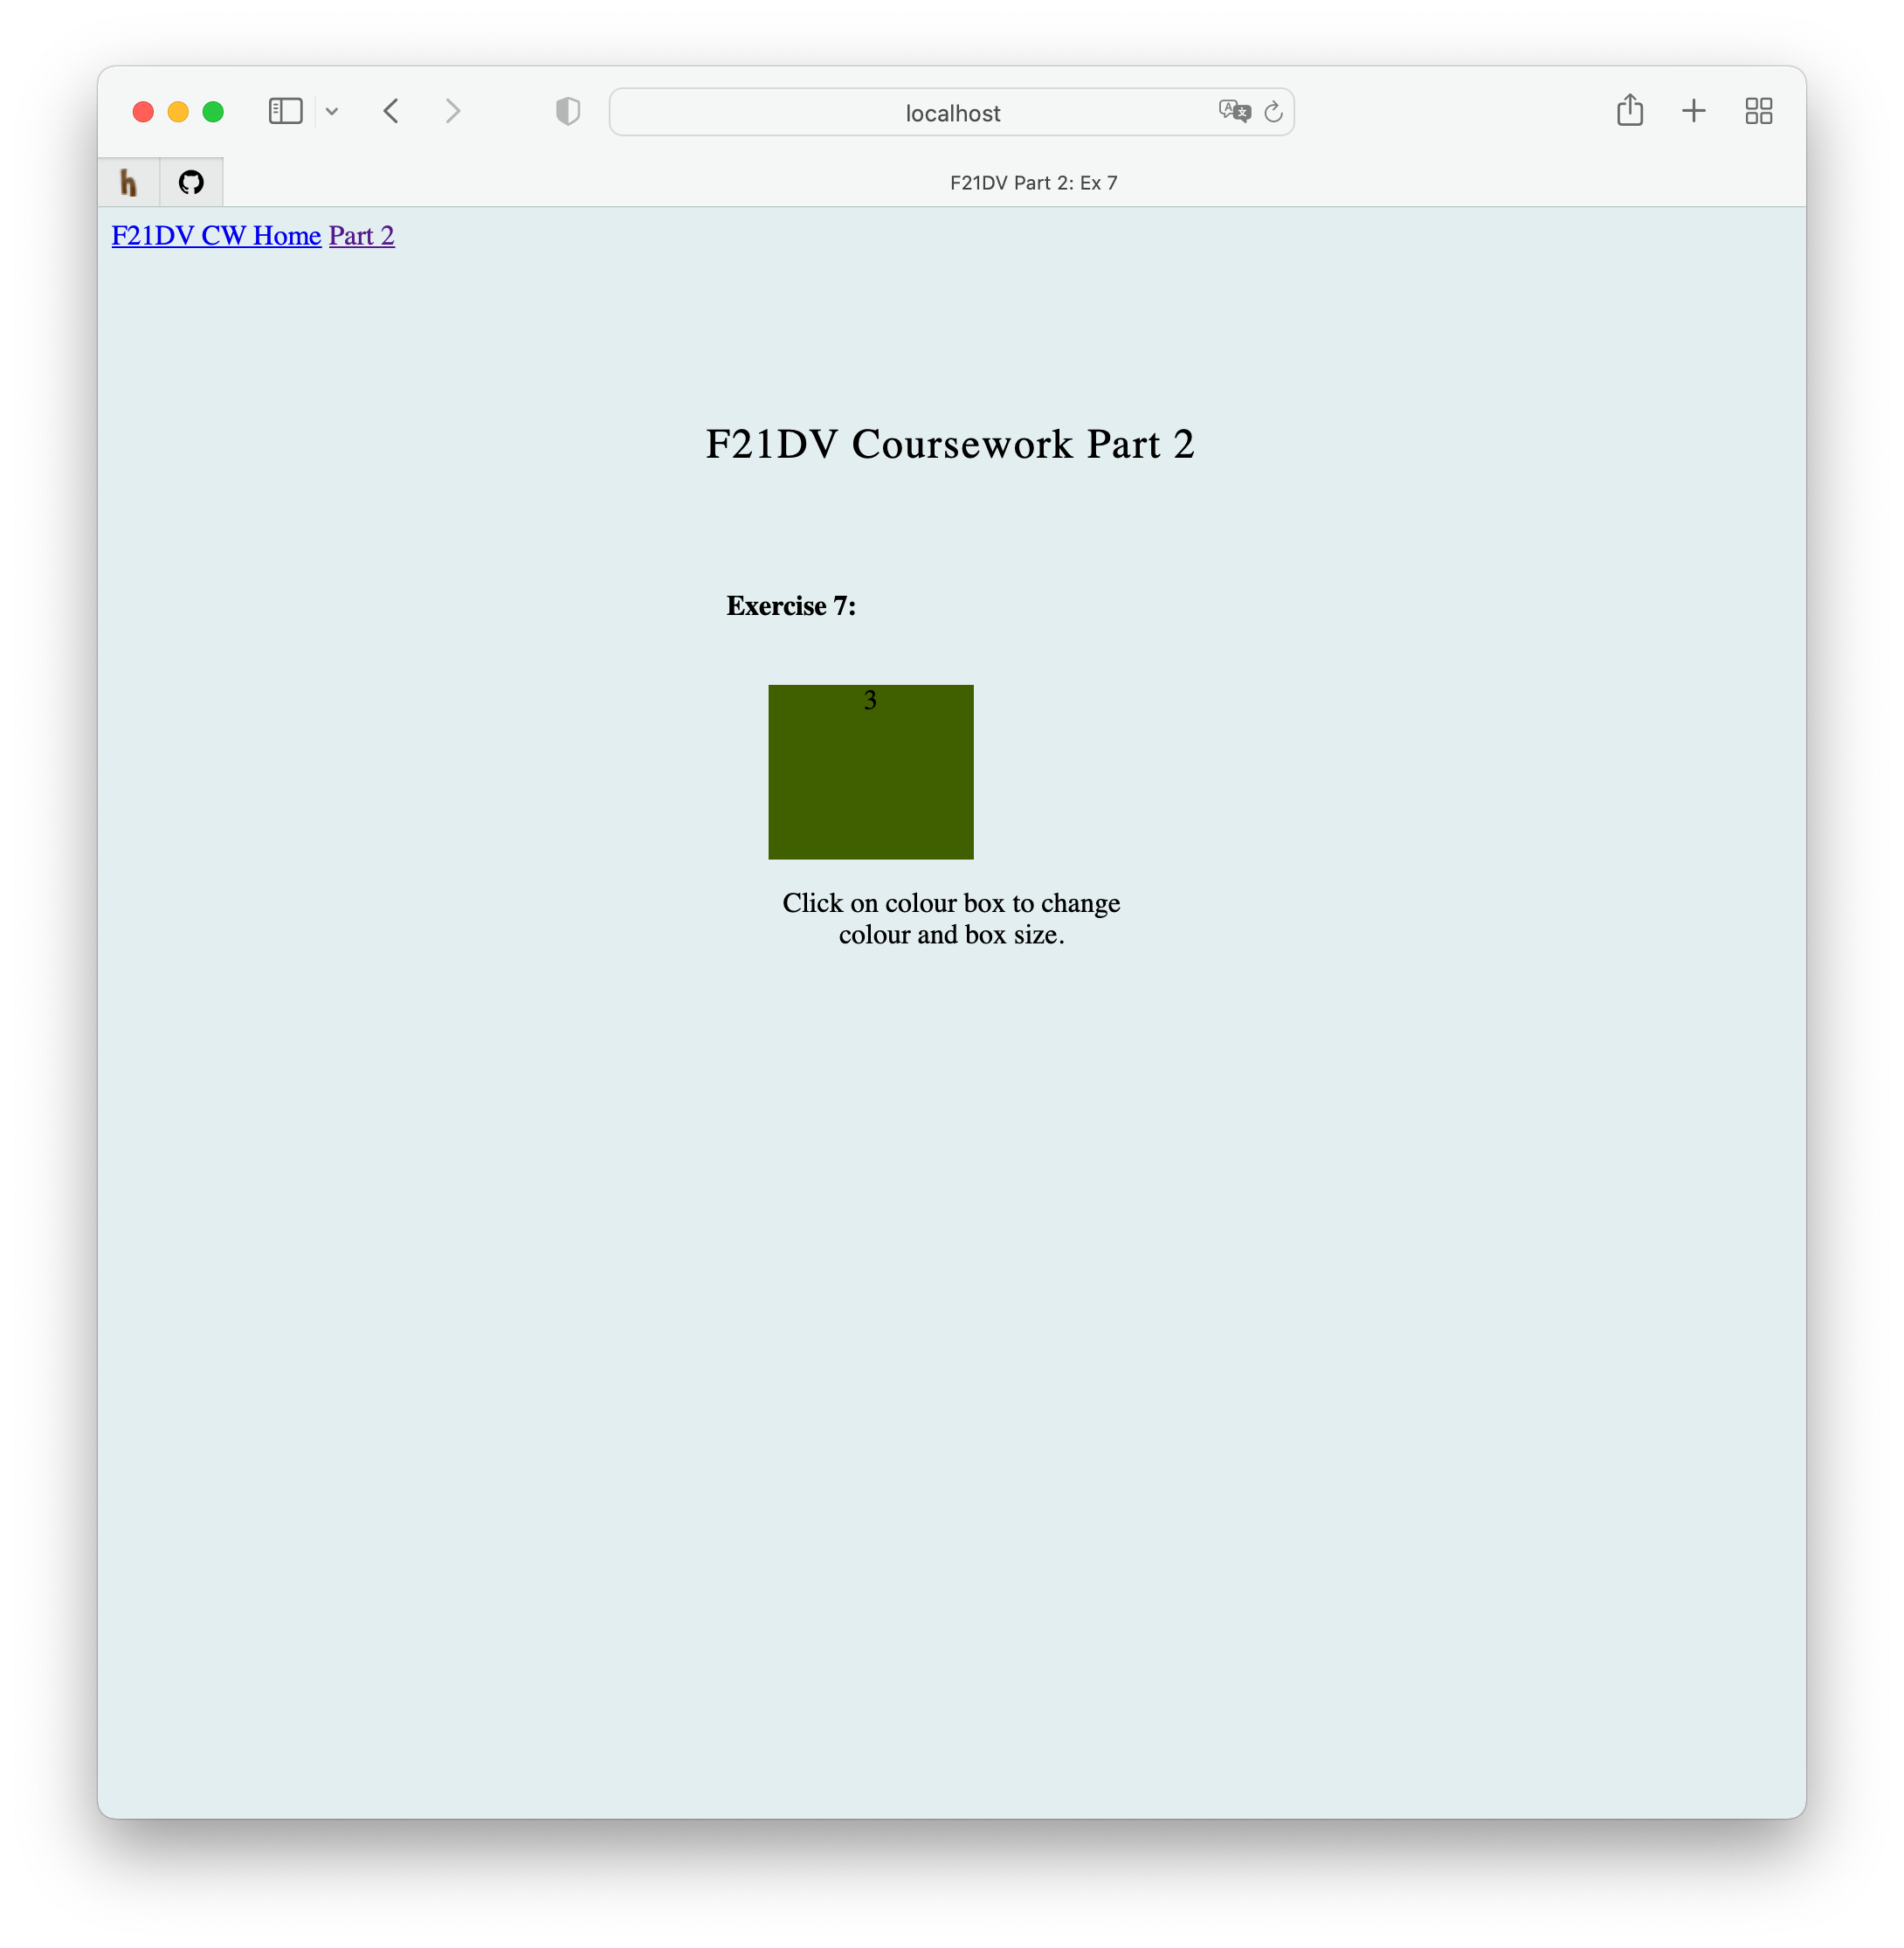
\includegraphics[width = 7.5cm]{images/ex7_3.png}
    \label{fig:ex7}
    \caption{Exercise 7}
\end{figure}
\FloatBarrier
% \lstinputlisting[language=JavaScript]{../../public/js/part2/task7.js}
Figure \ref{fig:ex7} shows the changes of a div upon clicking. This is pretty much the same as the one in exercise 6, except that I have added a transition to the size of the div.
\section{Exercise 8}
Exercise 8 is the same as 7, instead, the mouse action is now changed from click to hover.

\newpage
\section{Exercise 9}
\begin{figure}[!ht]
    \centering
    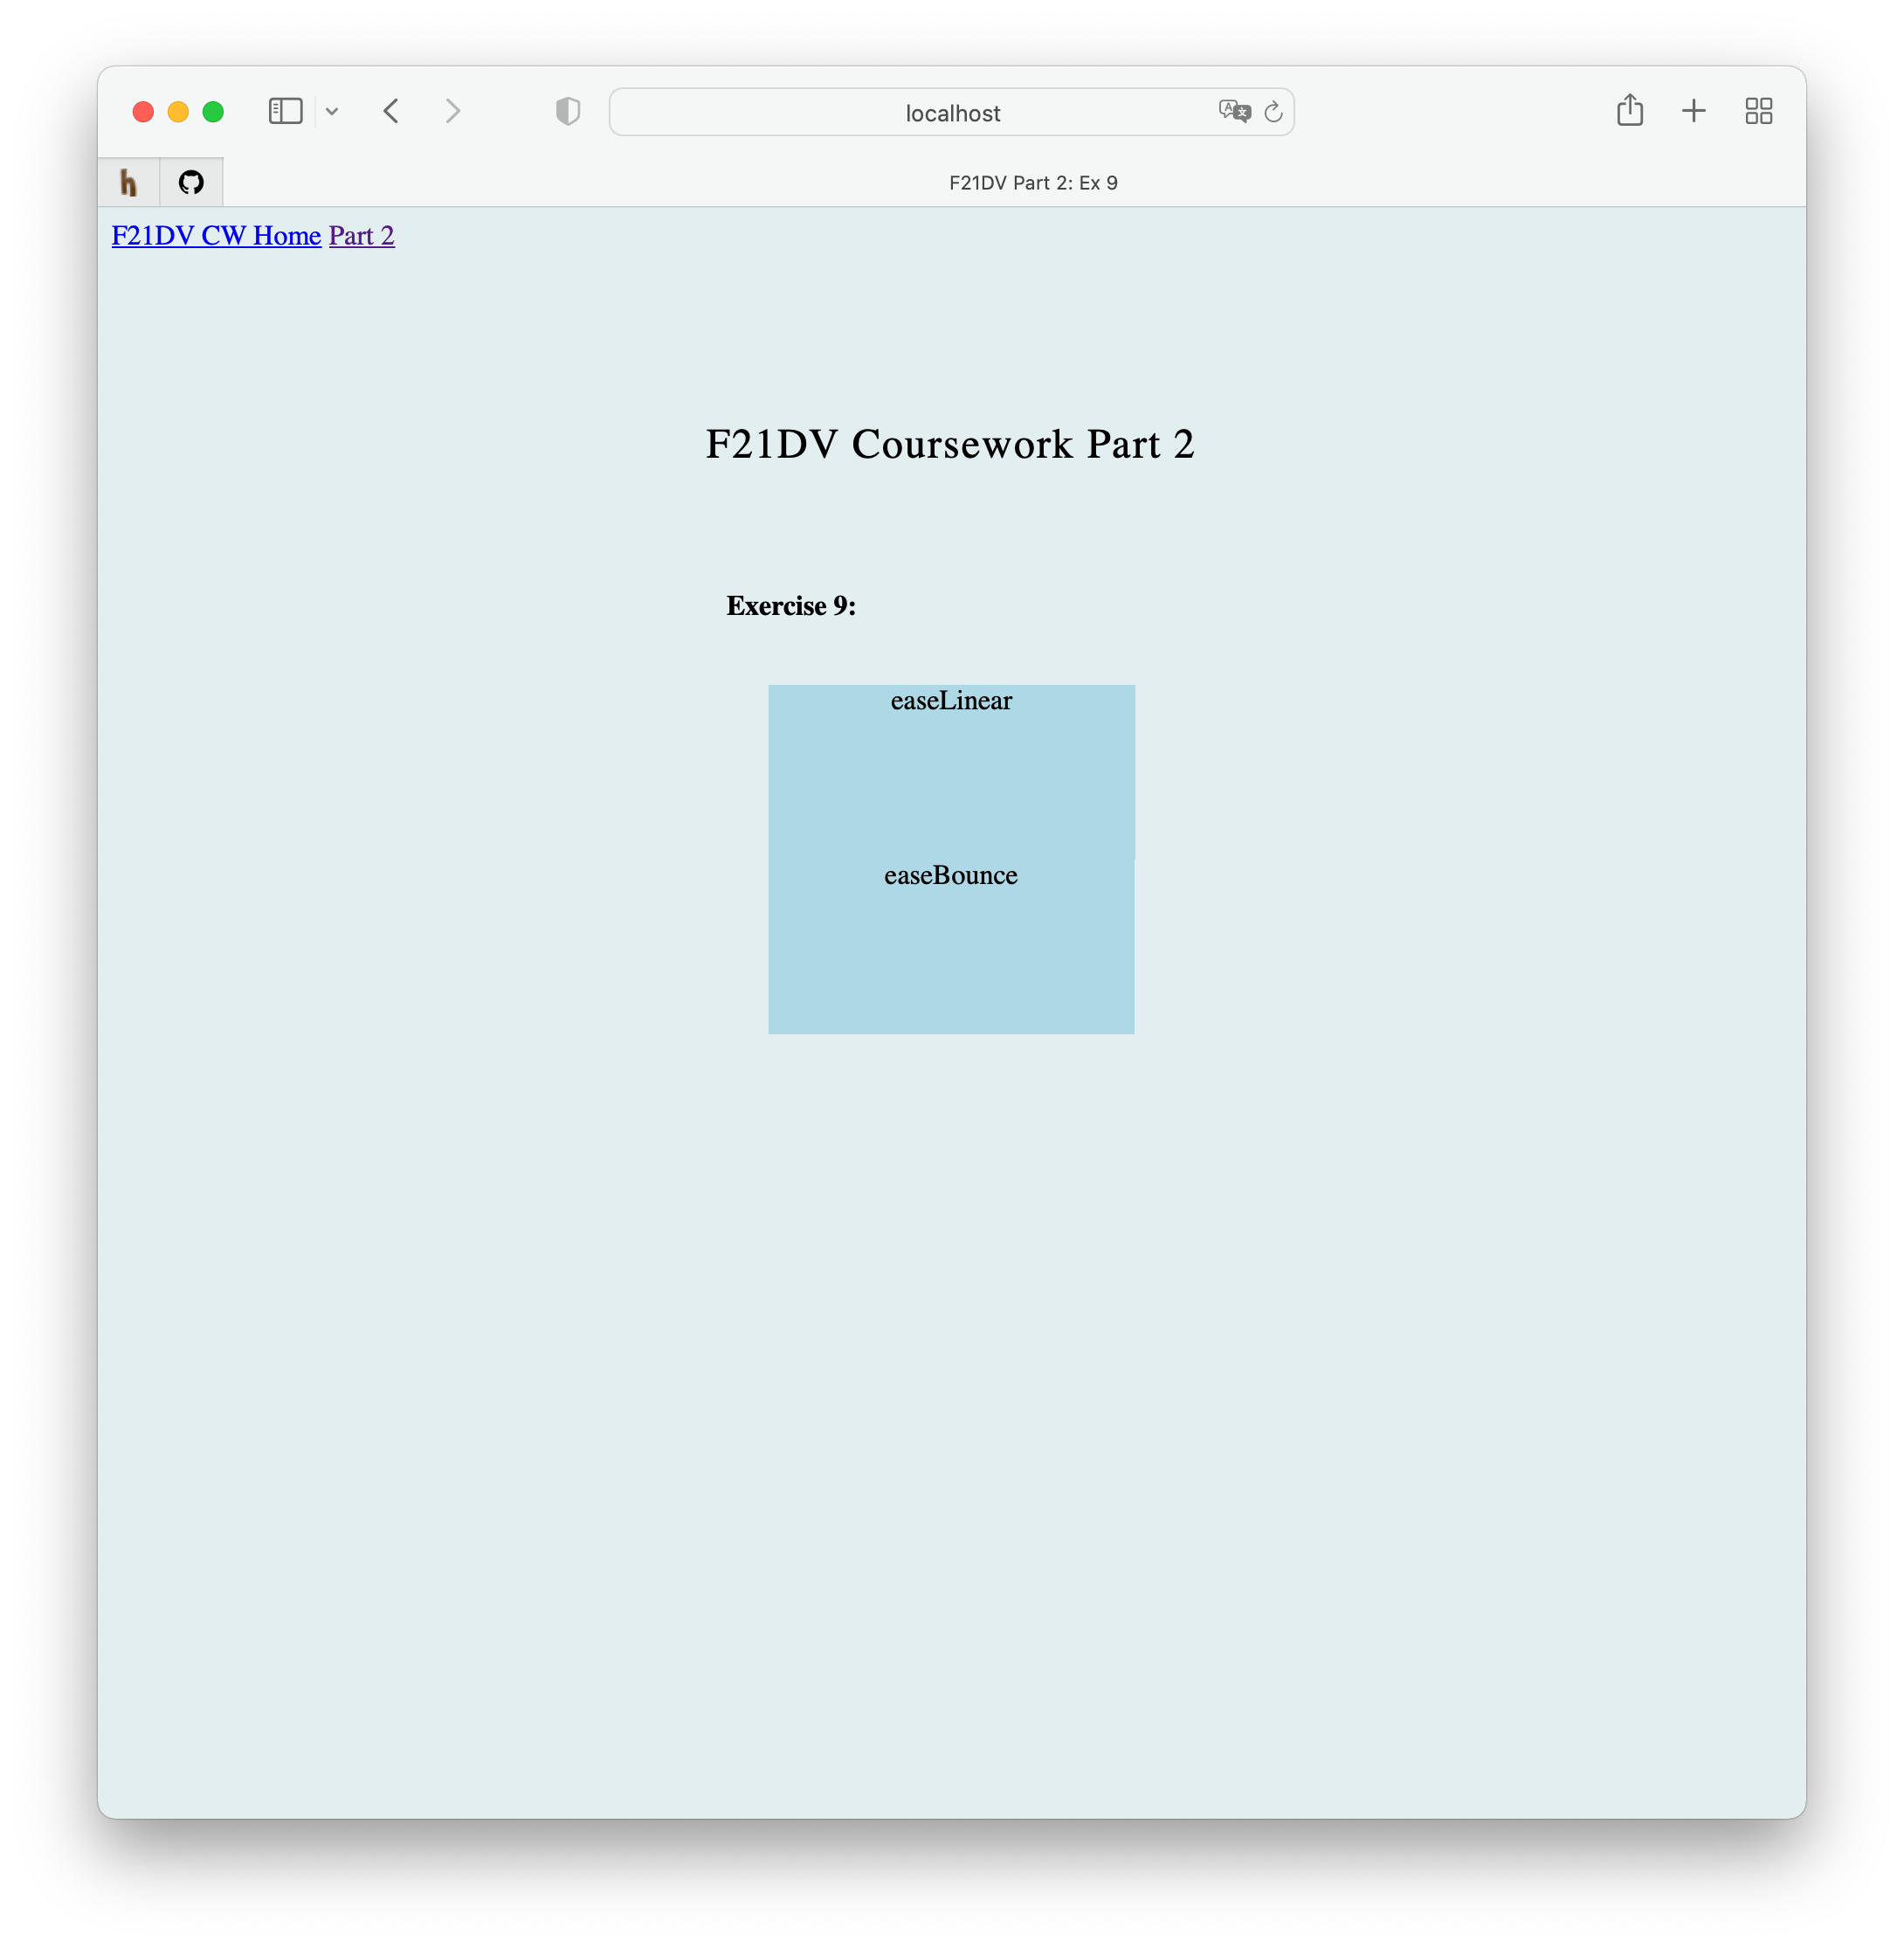
\includegraphics[width = 7.5cm]{images/ex9_1.png}
    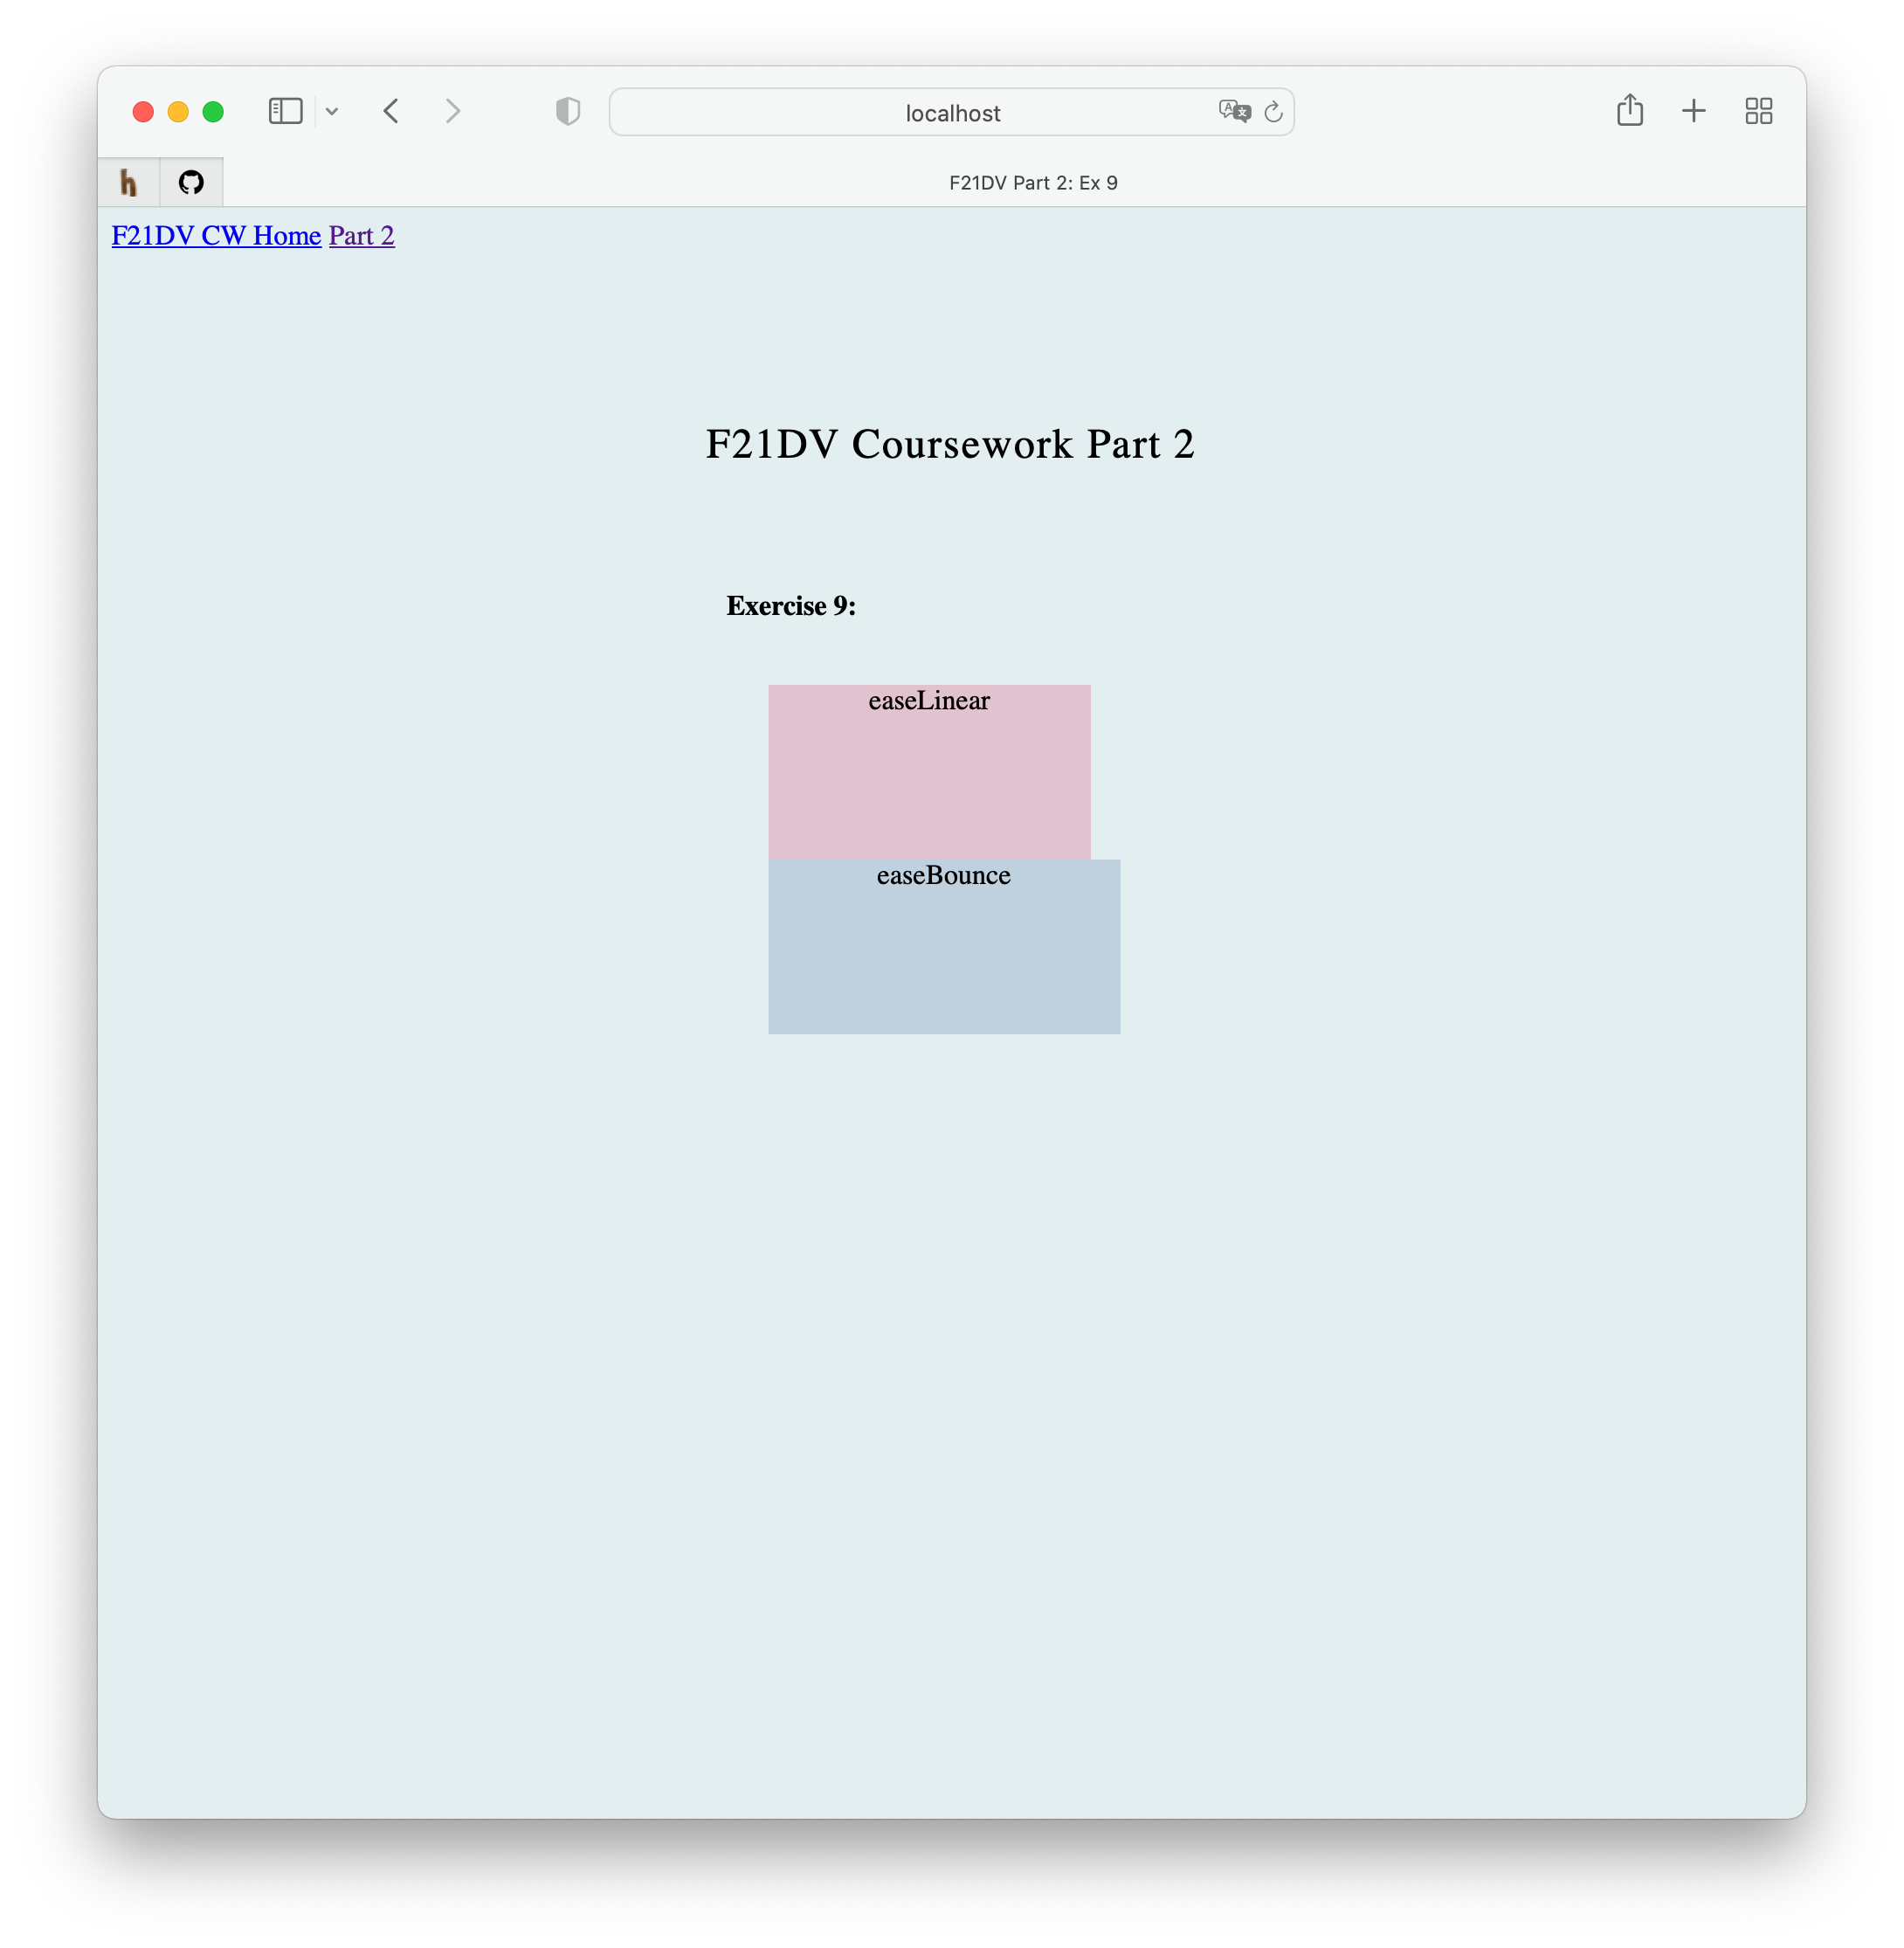
\includegraphics[width = 7.5cm]{images/ex9_2.png}
    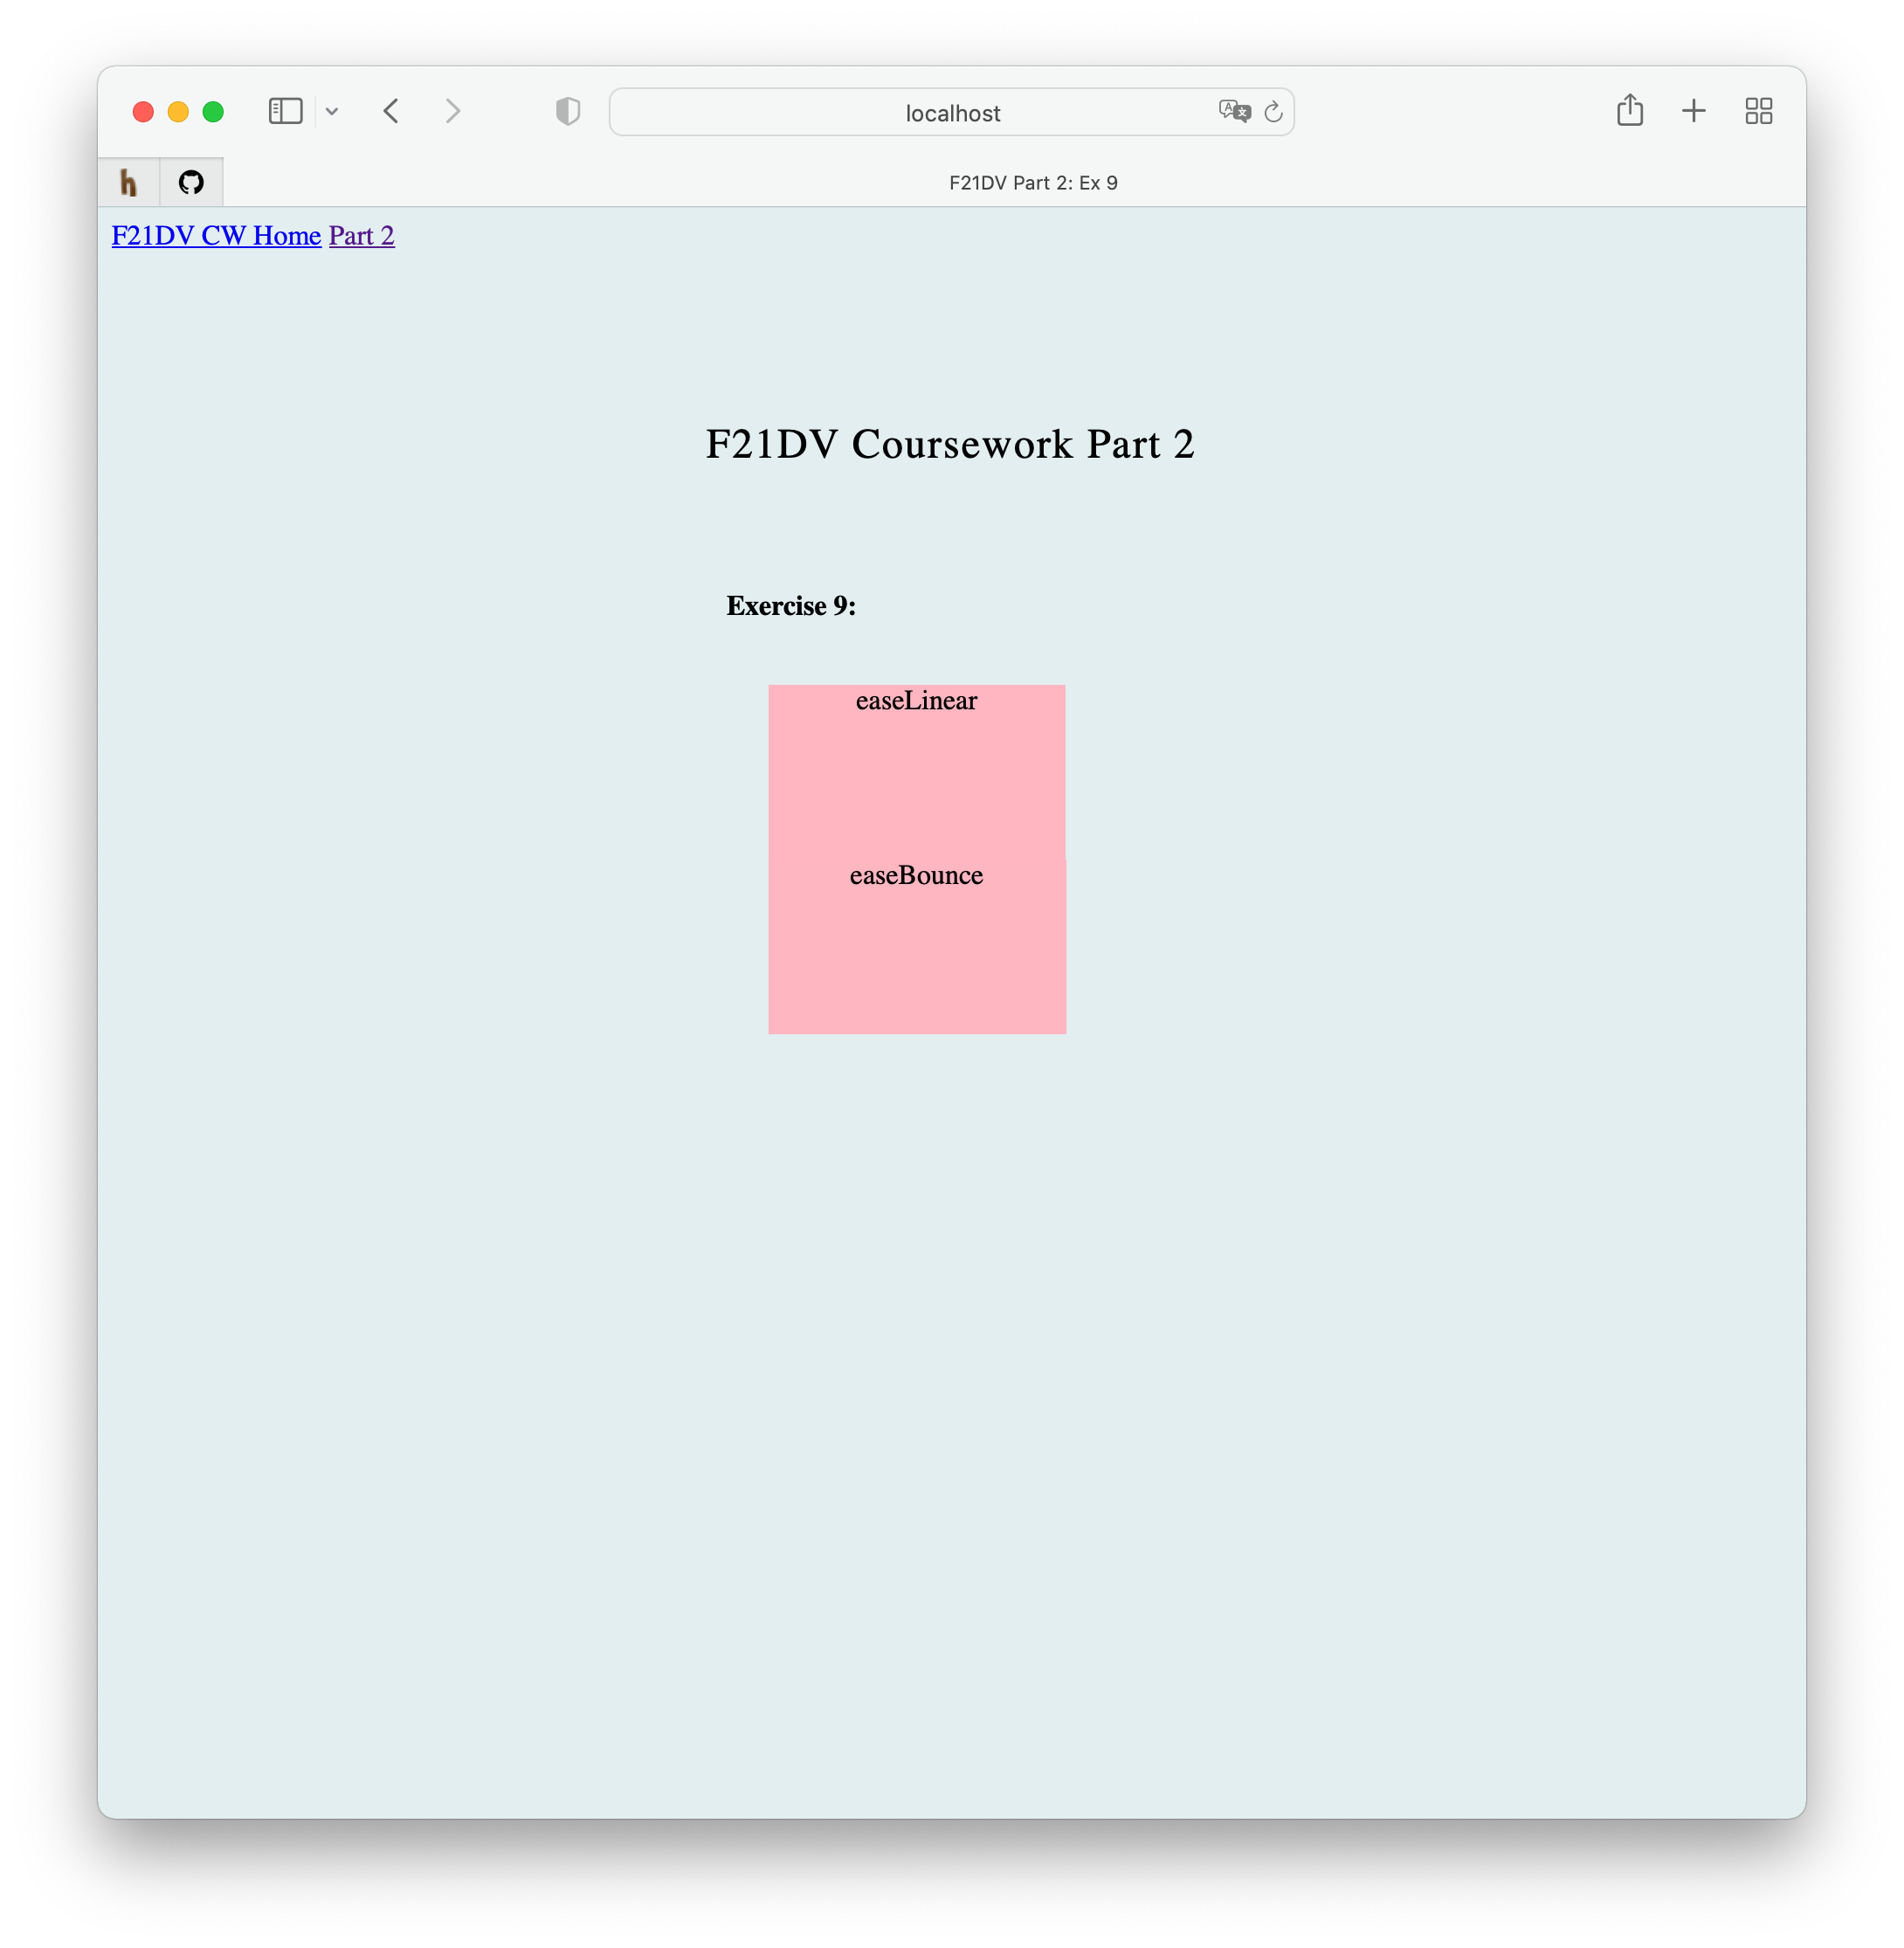
\includegraphics[width = 7.5cm]{images/ex9_3.png}
    \label{fig:ex9}
    \caption{Exercise 9}
\end{figure}
\FloatBarrier
% \lstinputlisting[language=JavaScript]{../../public/js/part2/task7.js}
Figure \ref{fig:ex9} shows the difference in the transition ease method. The figure shows two divs, one using the \verb|d3.easeLinear| method and the other using \verb|d3.easeBounce|. Both divs have the same transition endpoint and duration, but in between, due to the different ease method they woudl appear differently as shown in the second picture. This page also uses the d3 \verb|.on(`end', ...)| function, which allows the transtion to start on load of the page, and just loop through.

\newpage
\section{Exercise 11}
\begin{figure}[!ht]
    \centering
    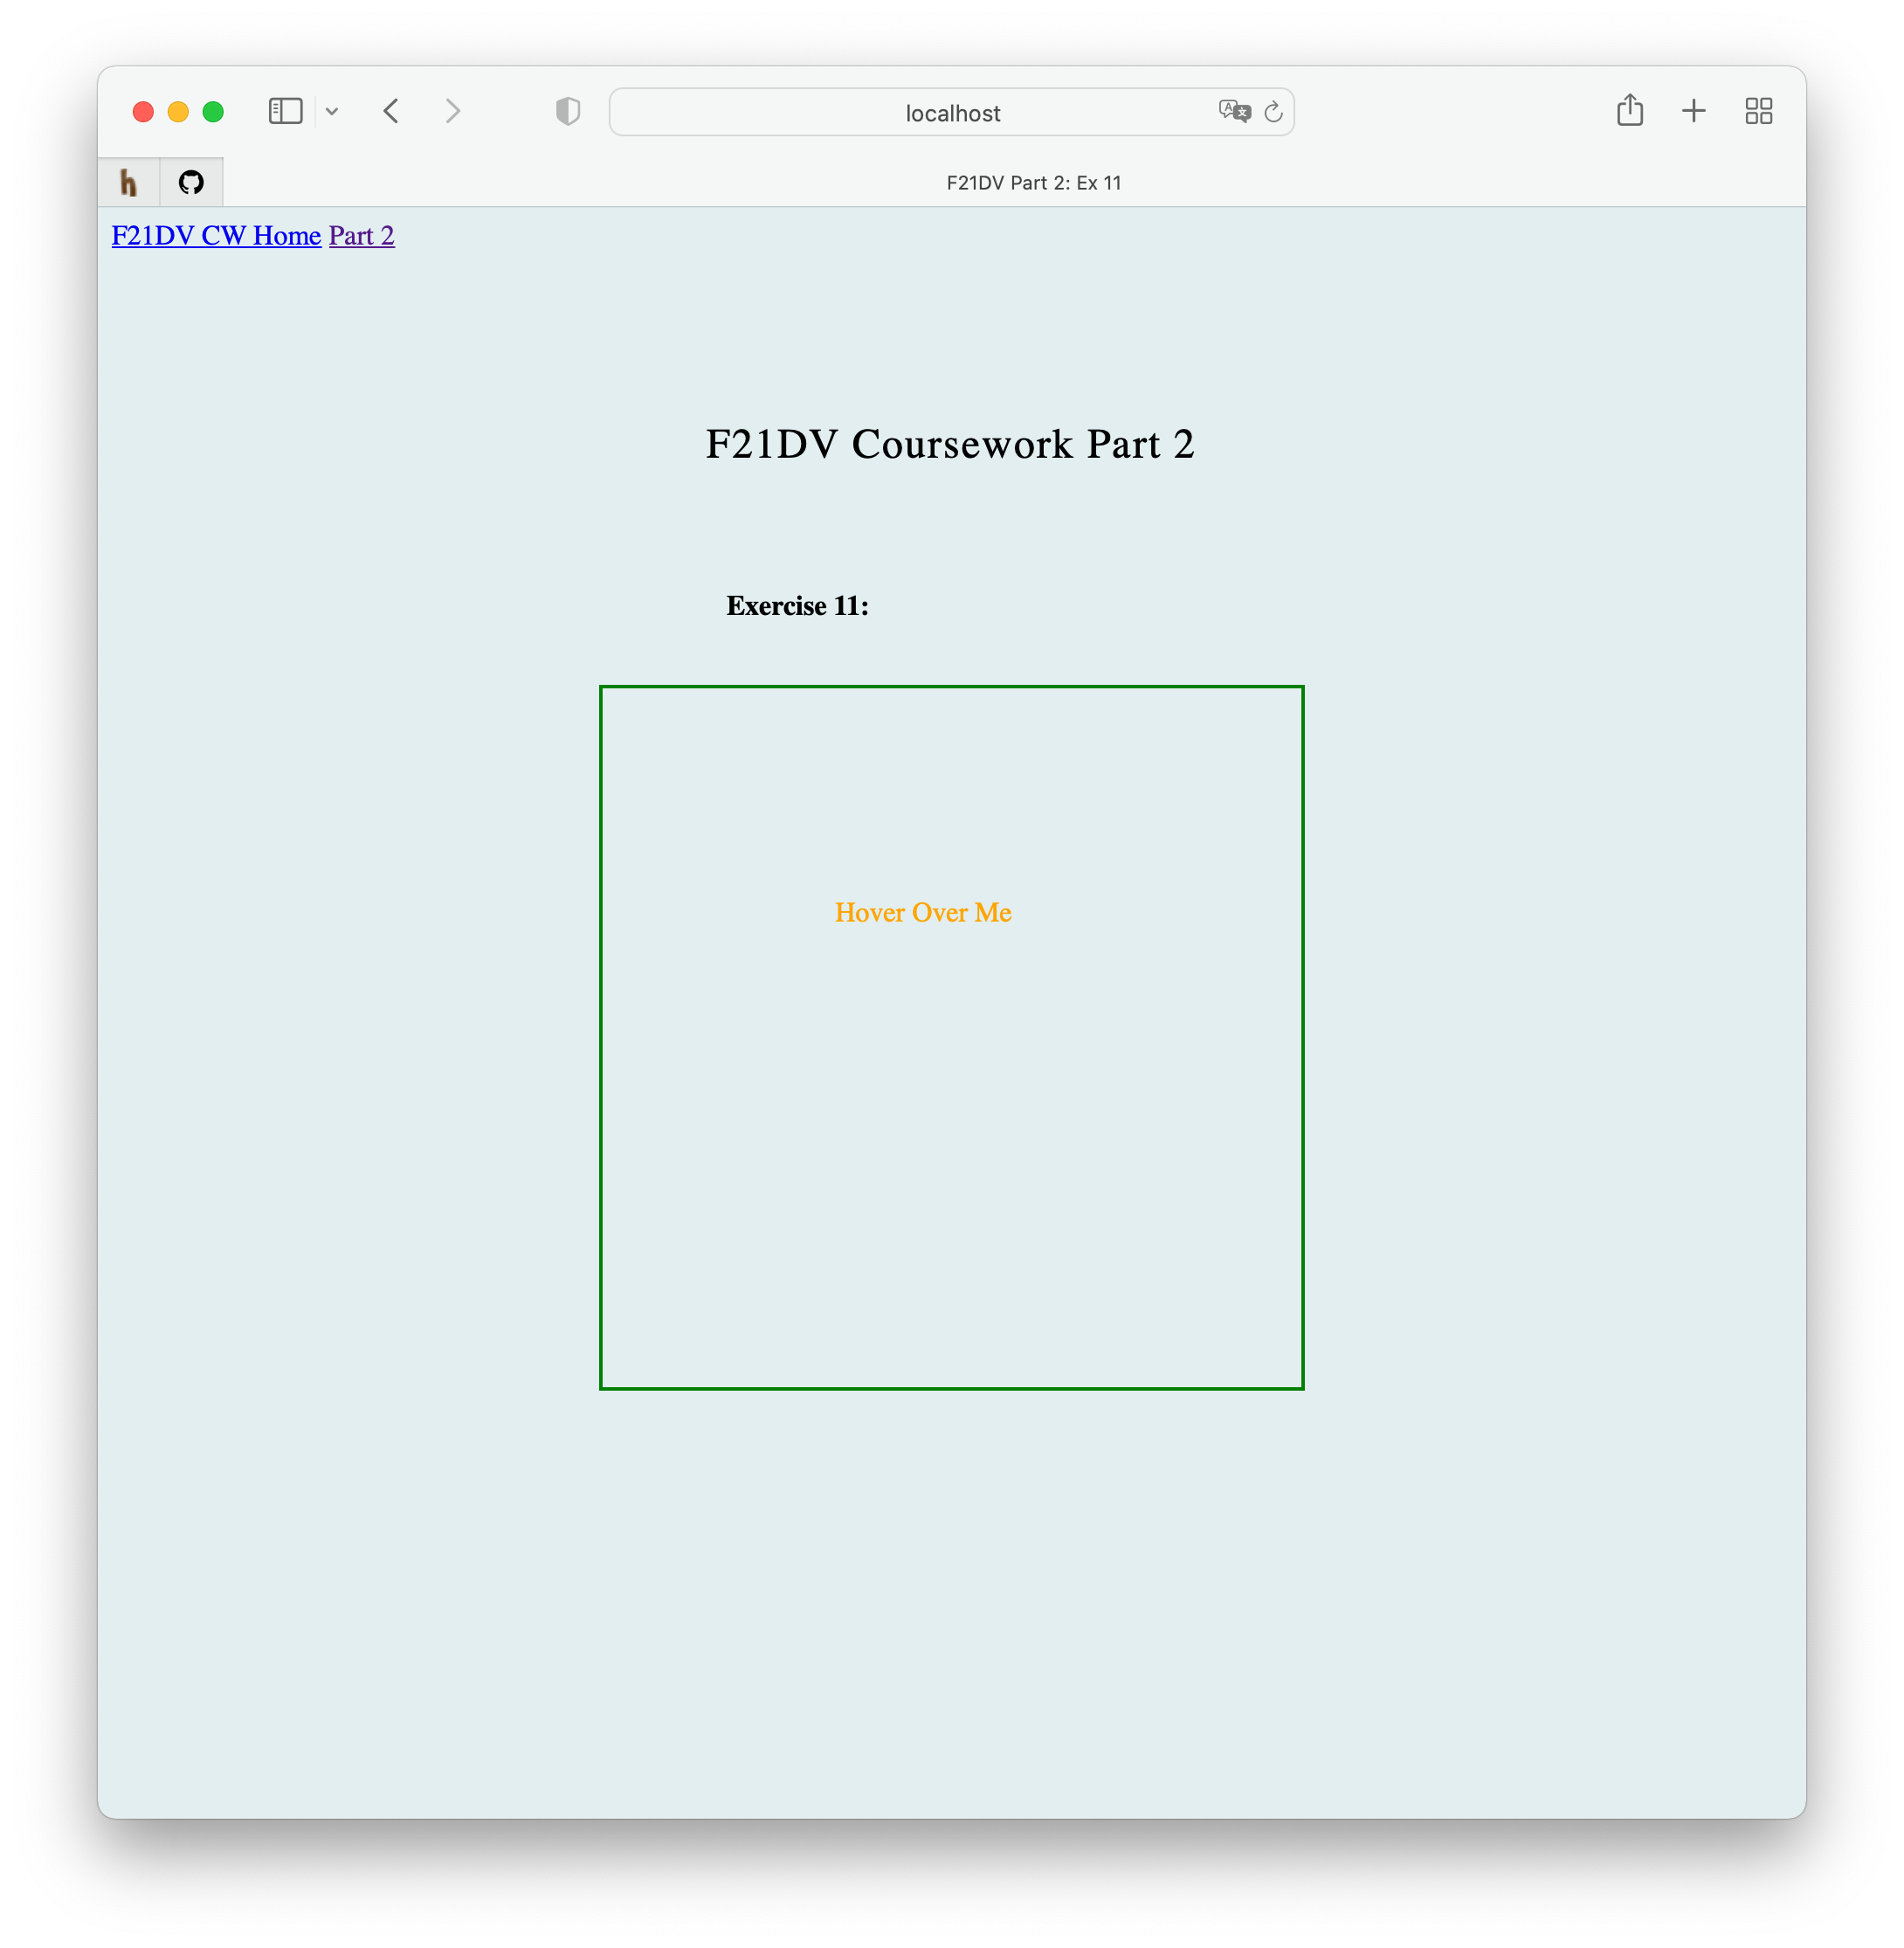
\includegraphics[width = 7.5cm]{images/ex11_1.png}
    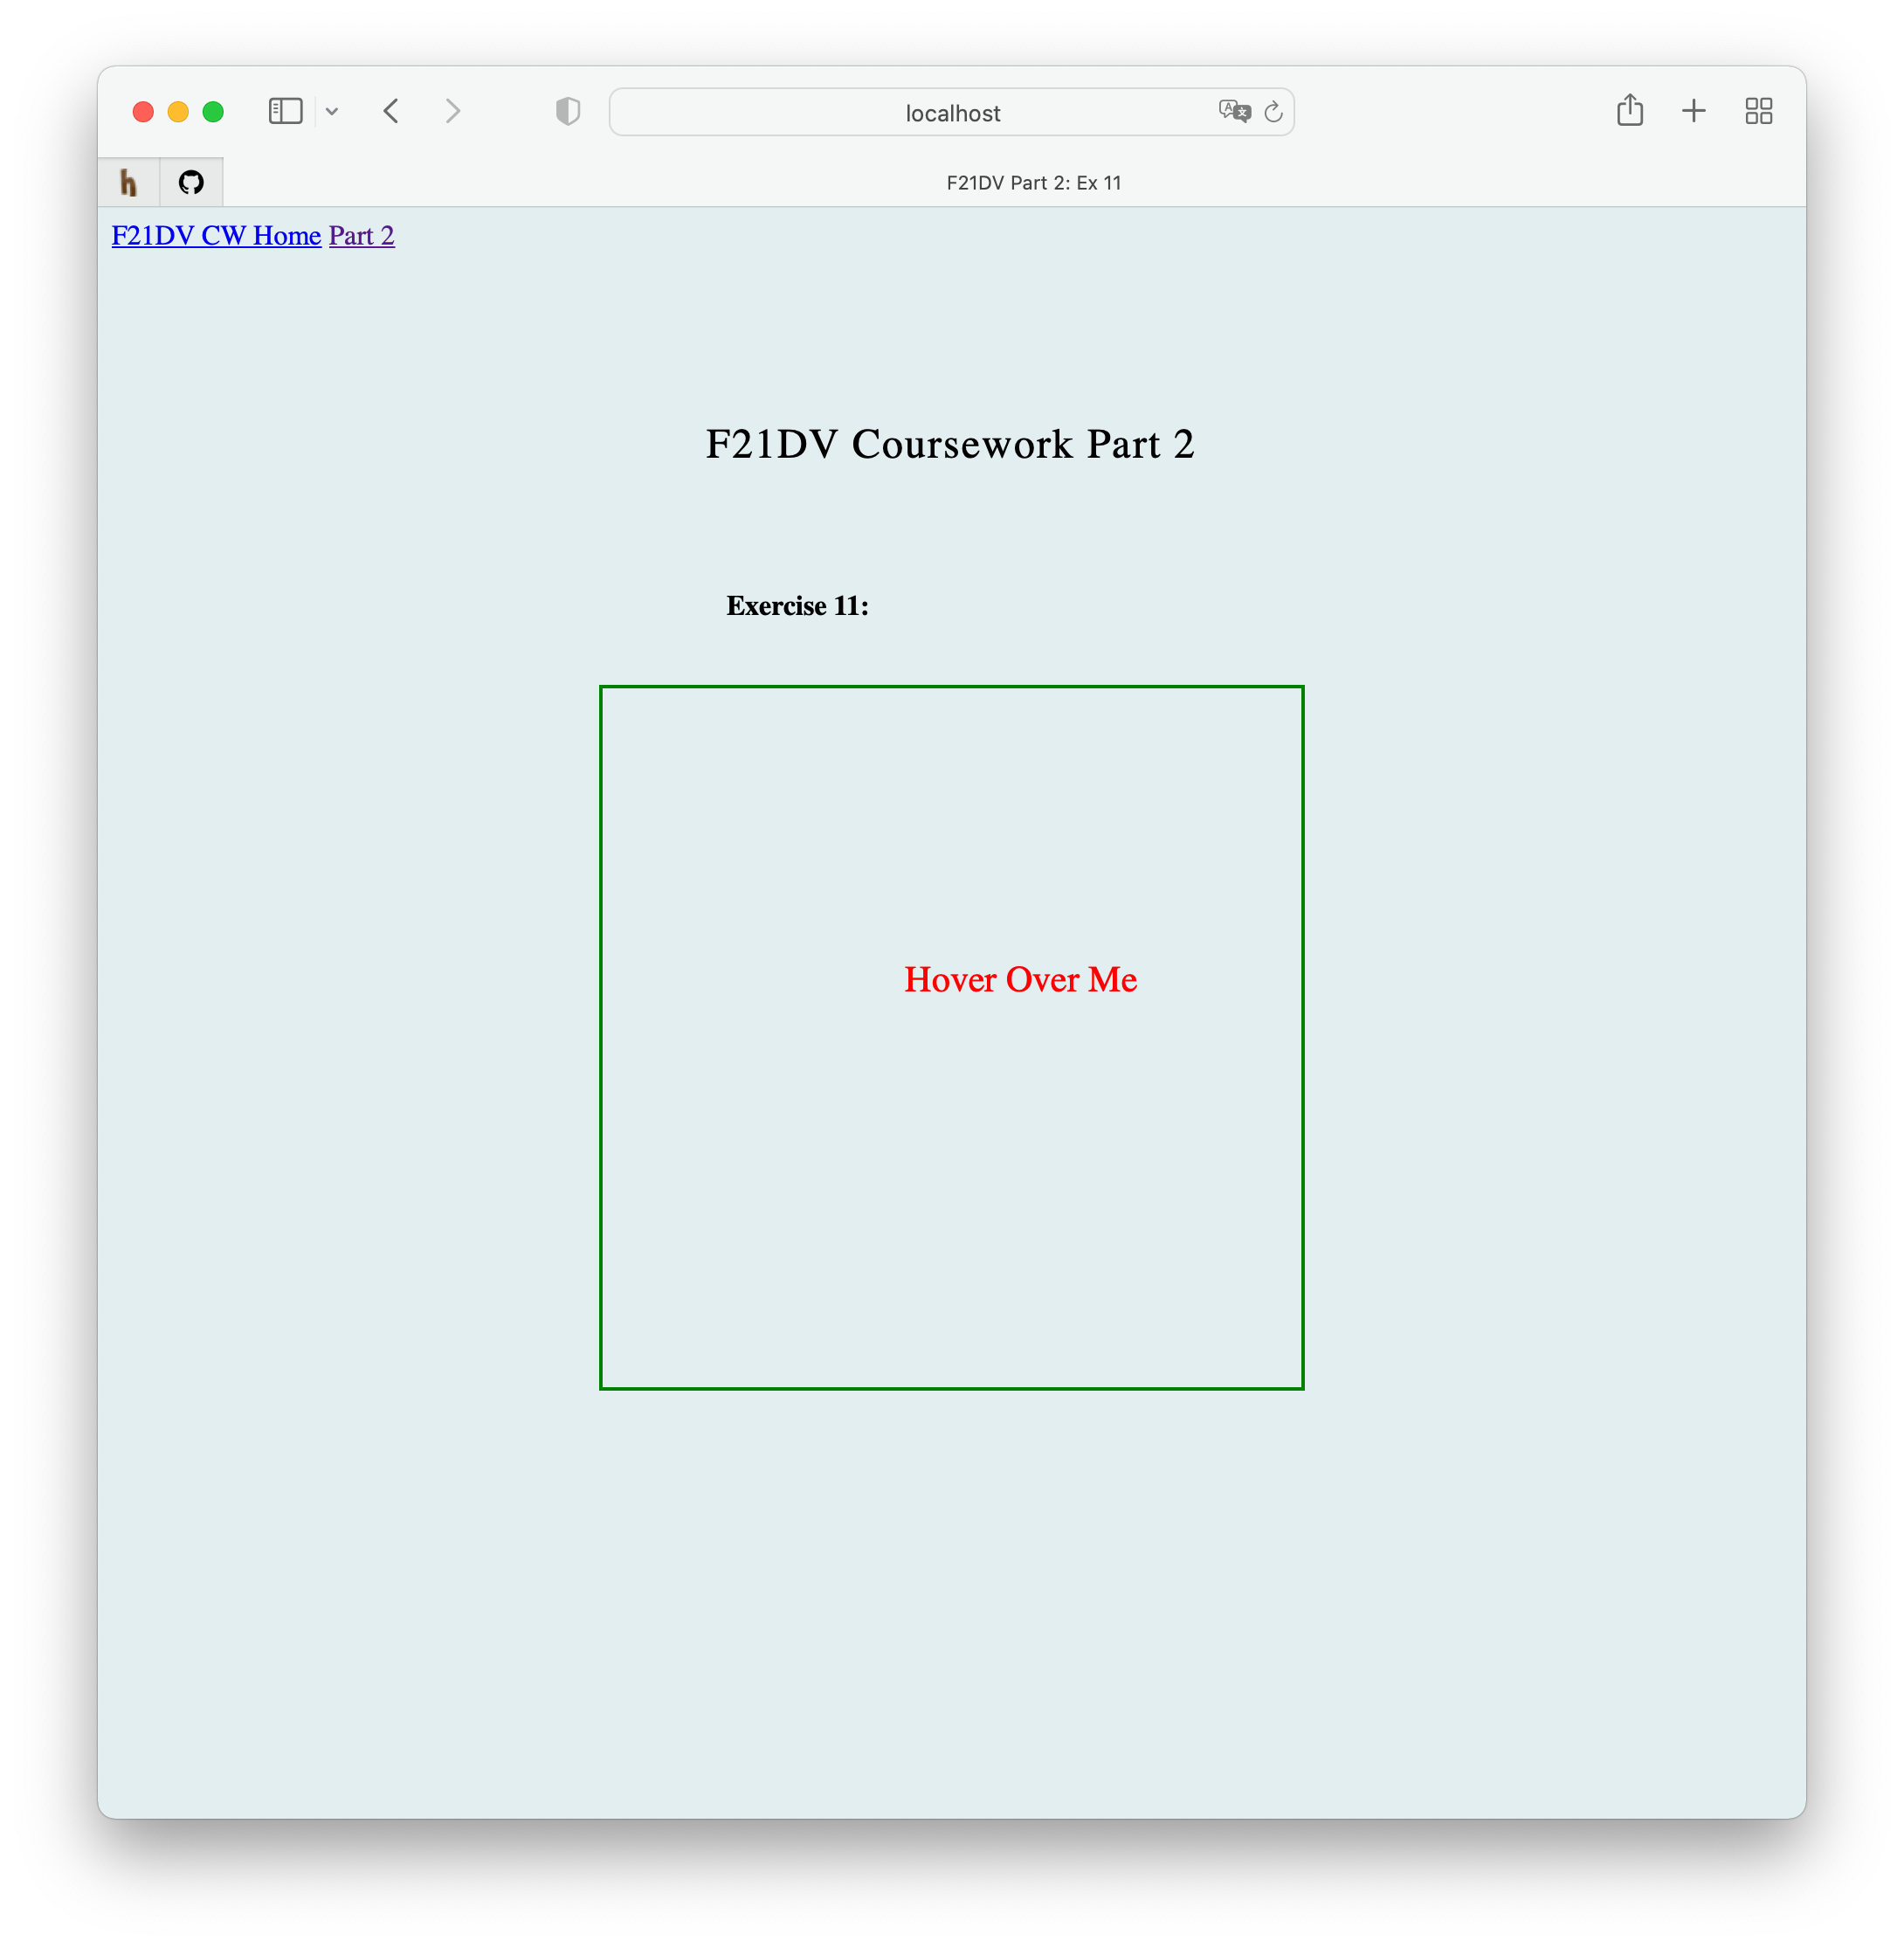
\includegraphics[width = 7.5cm]{images/ex11_2.png}
    % 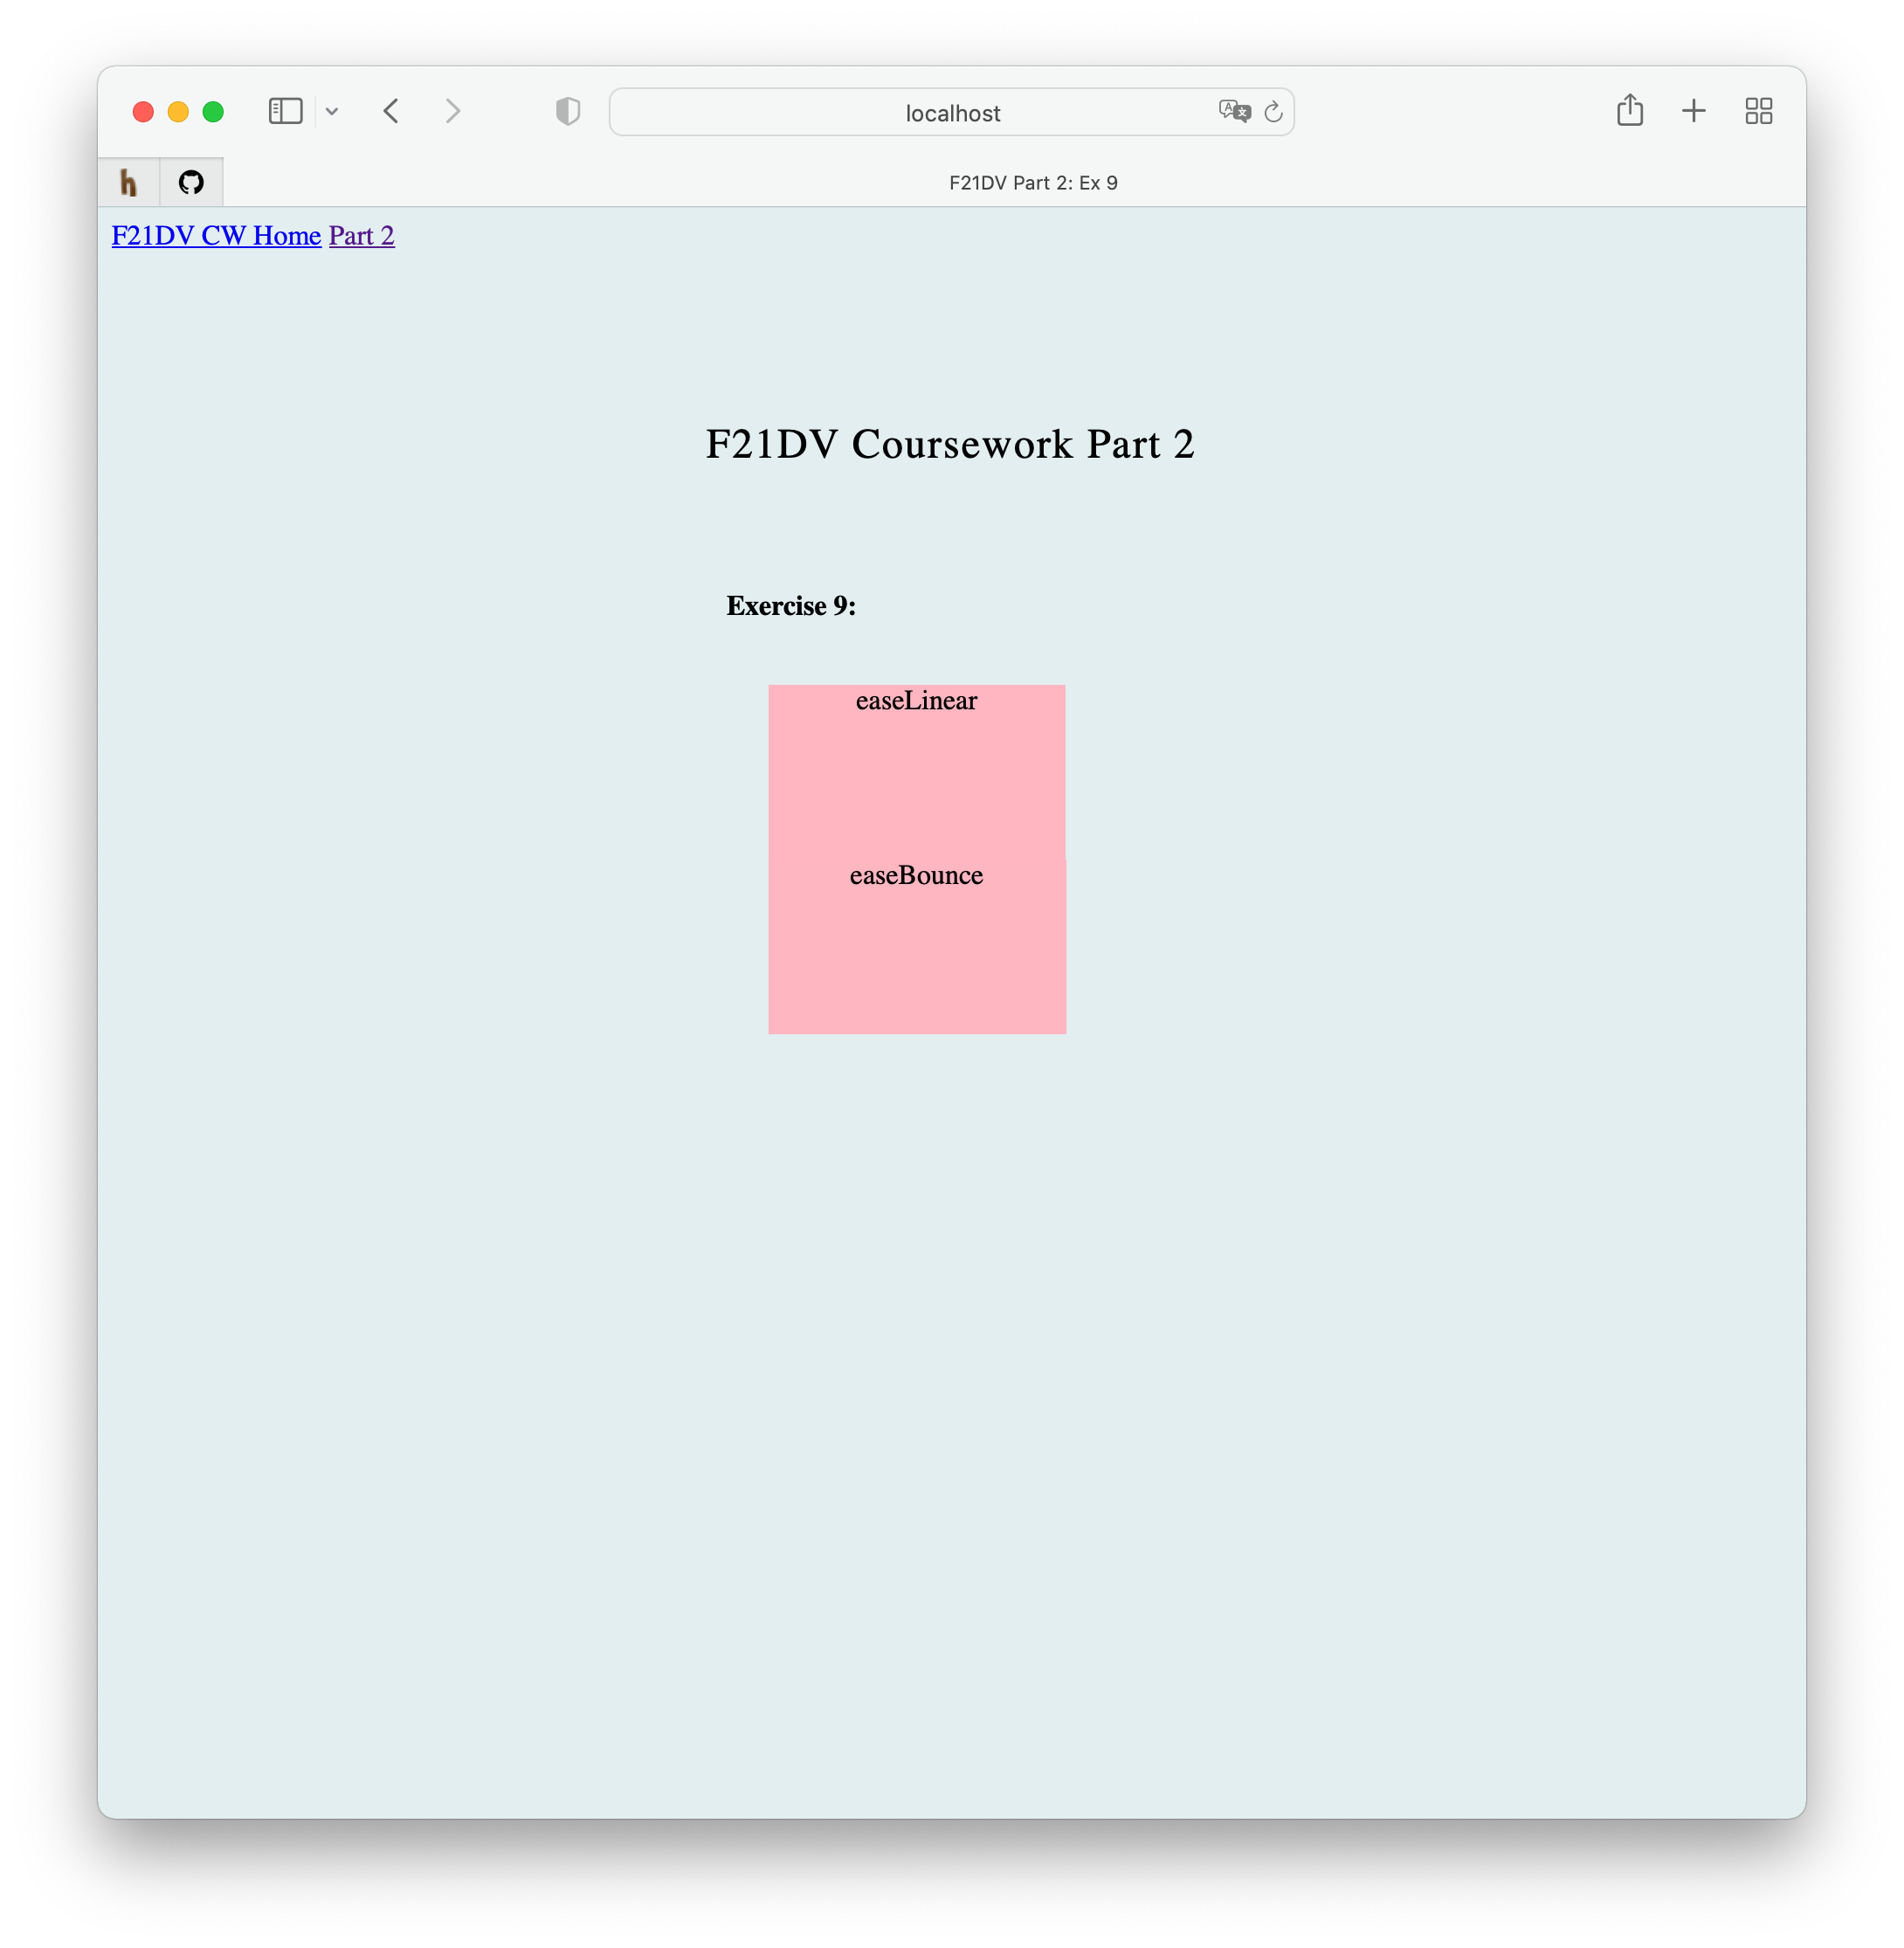
\includegraphics[width = 7.5cm]{images/ex9_3.png}
    \label{fig:ex11}
    \caption{Exercise 11}
\end{figure}
\FloatBarrier
% \lstinputlisting[language=JavaScript]{../../public/js/part2/task7.js}
Figure \ref{fig:ex11} shows a text on an svg, that changes colour and size on hover, and reverts back to its original state after the mouse leaves.

\newpage
\section{Exercise 12}
\begin{figure}[!ht]
    \centering
    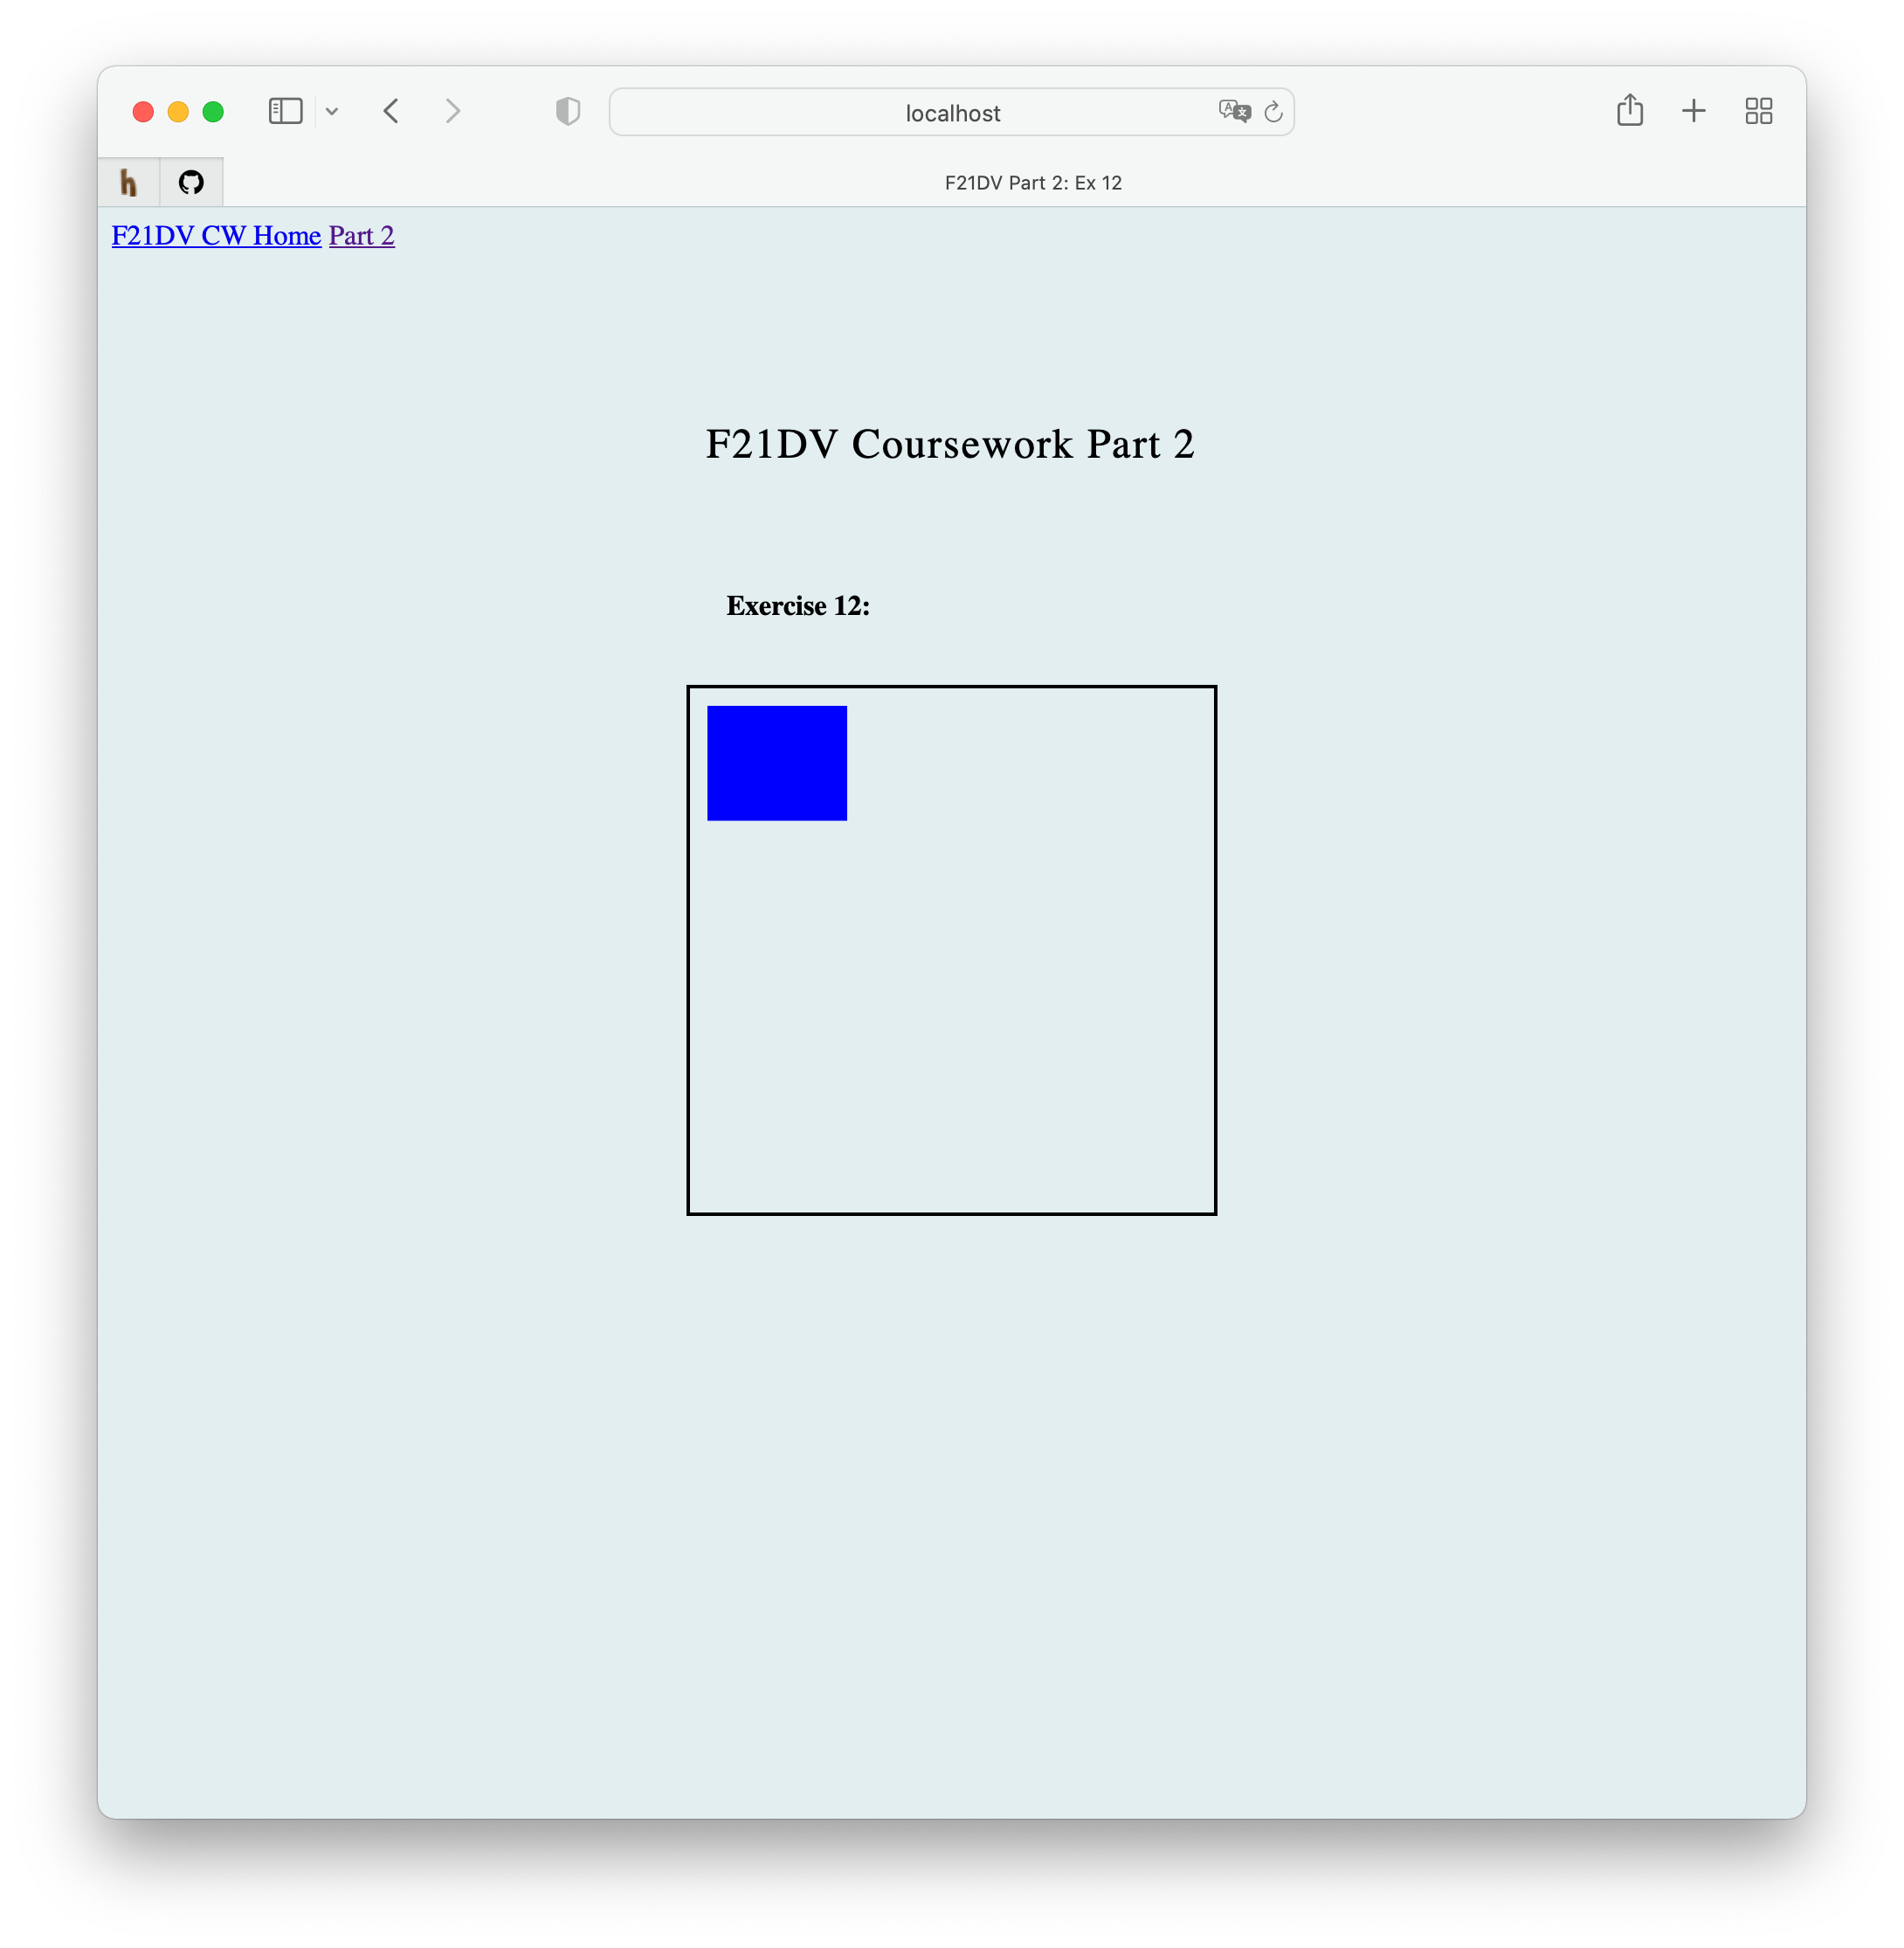
\includegraphics[width = 7.5cm]{images/ex12_1.png}
    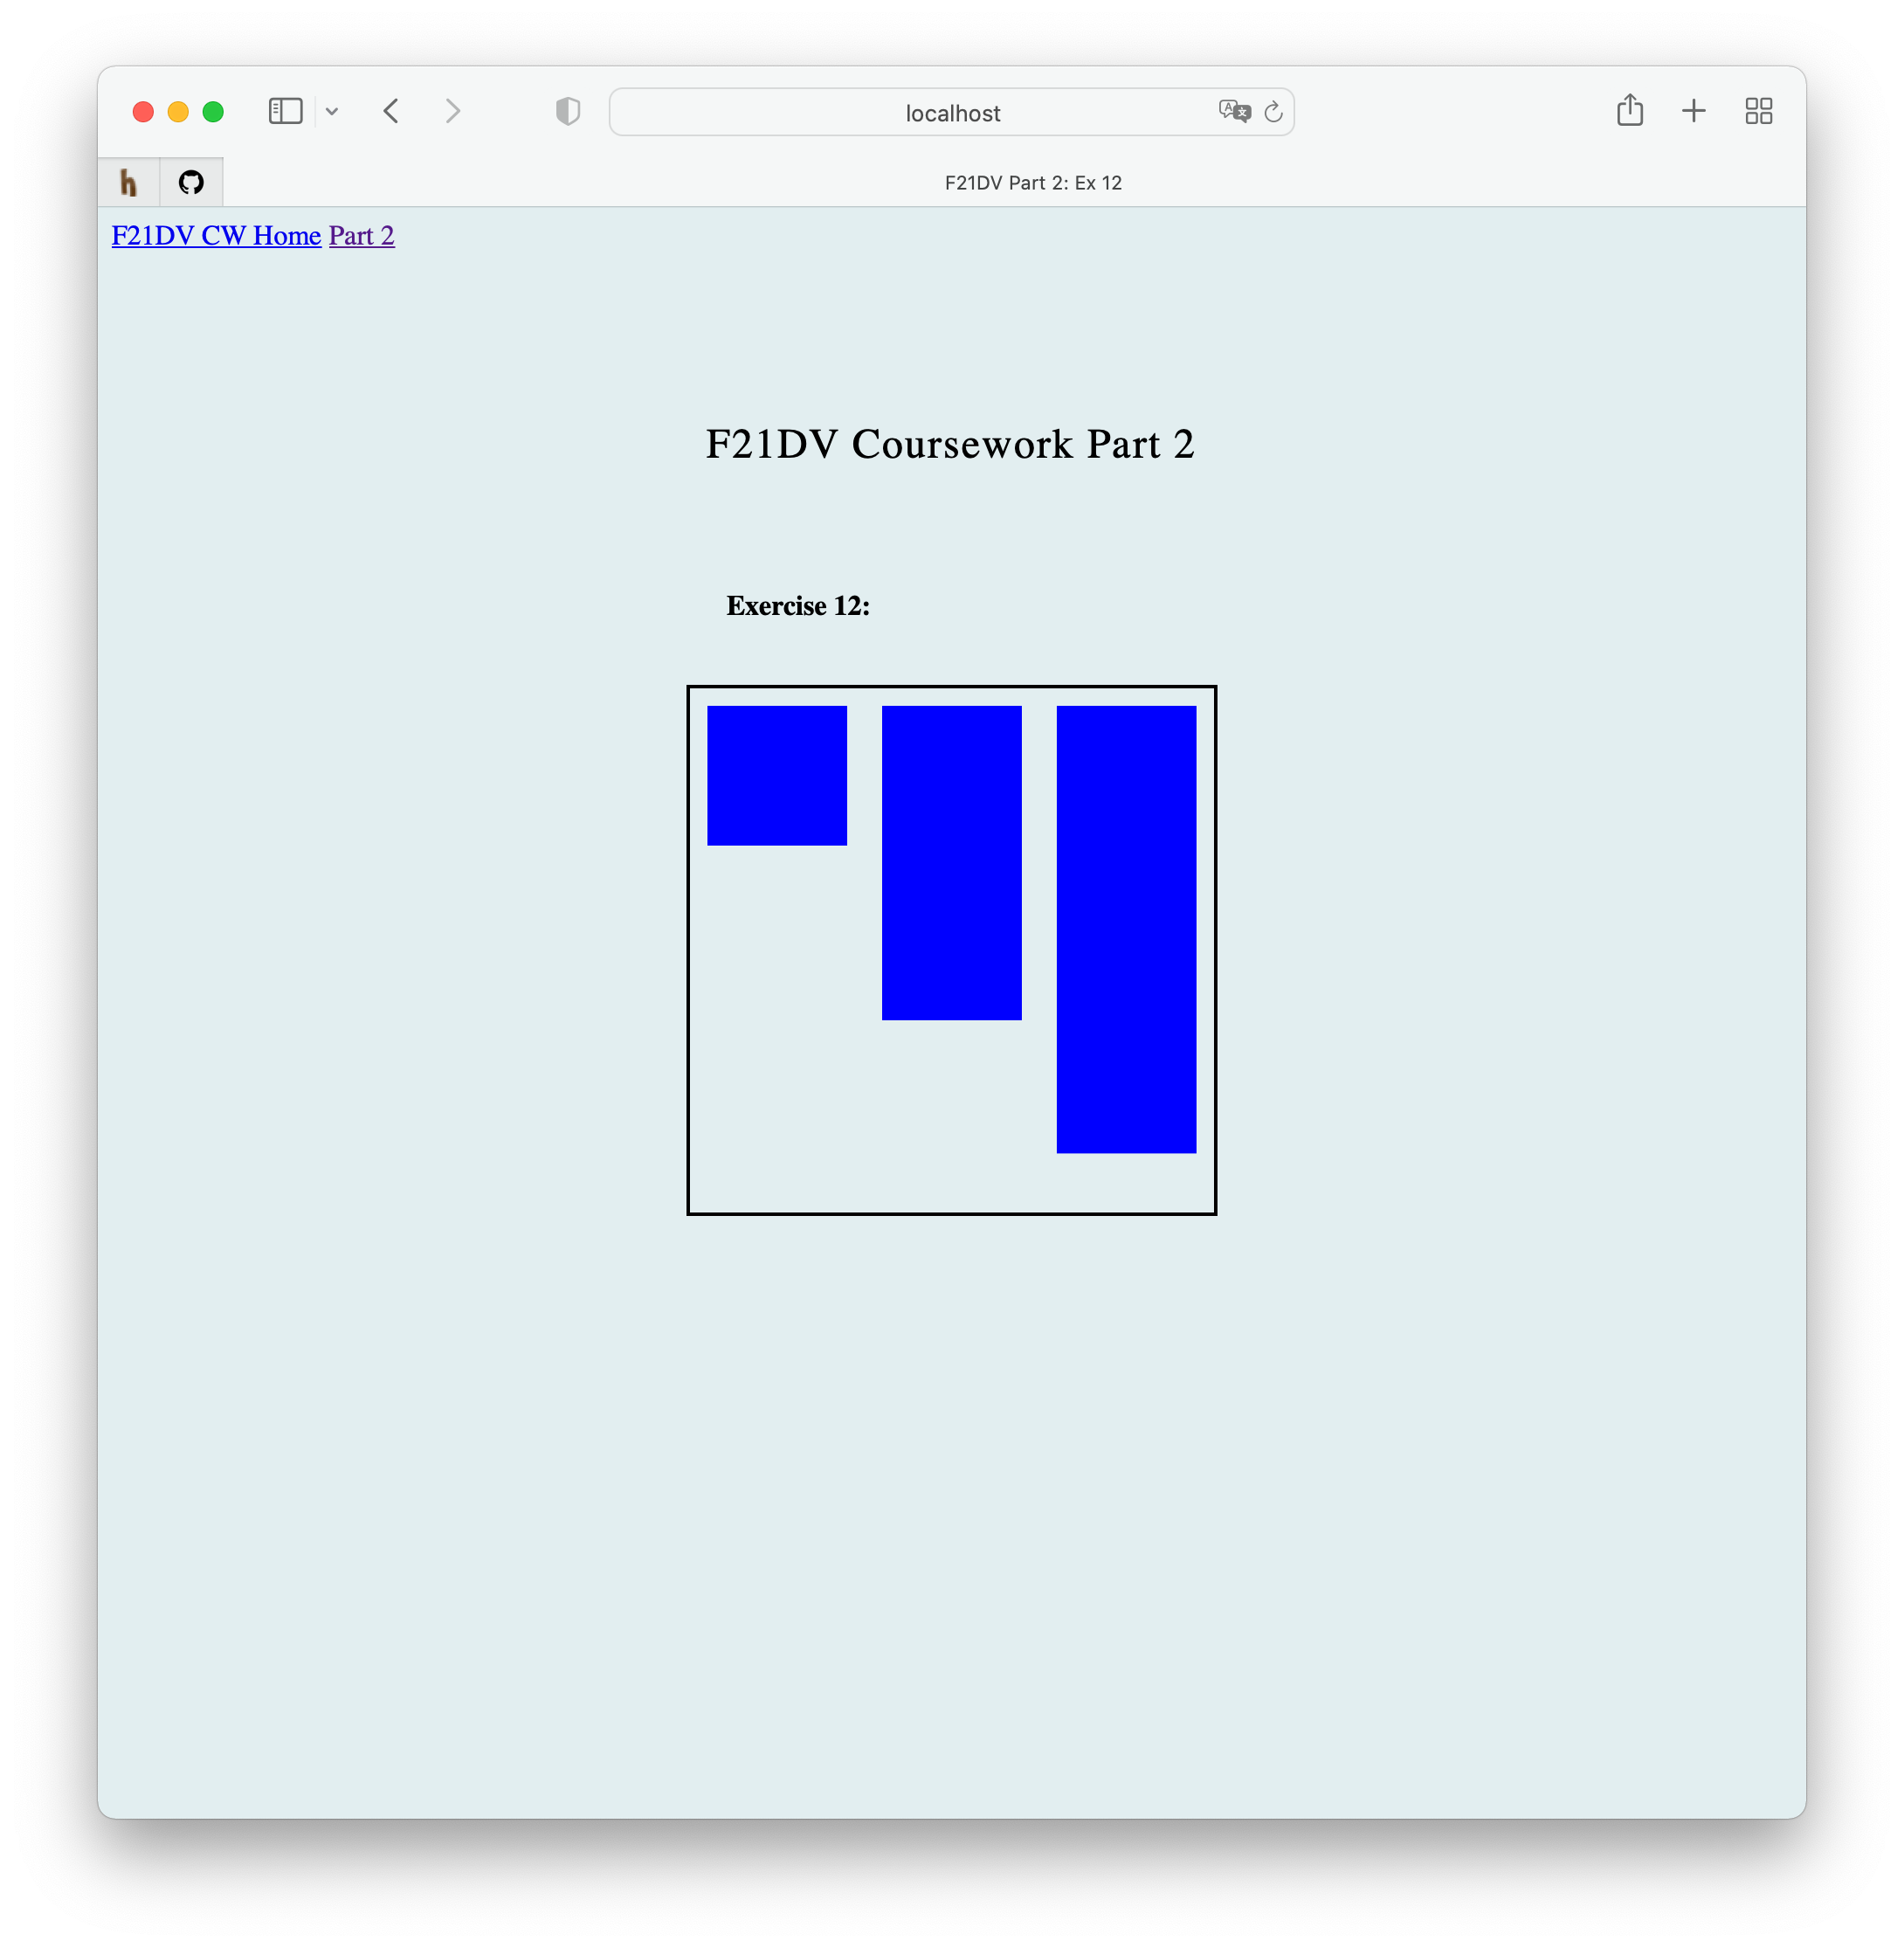
\includegraphics[width = 7.5cm]{images/ex12_2.png}
    % 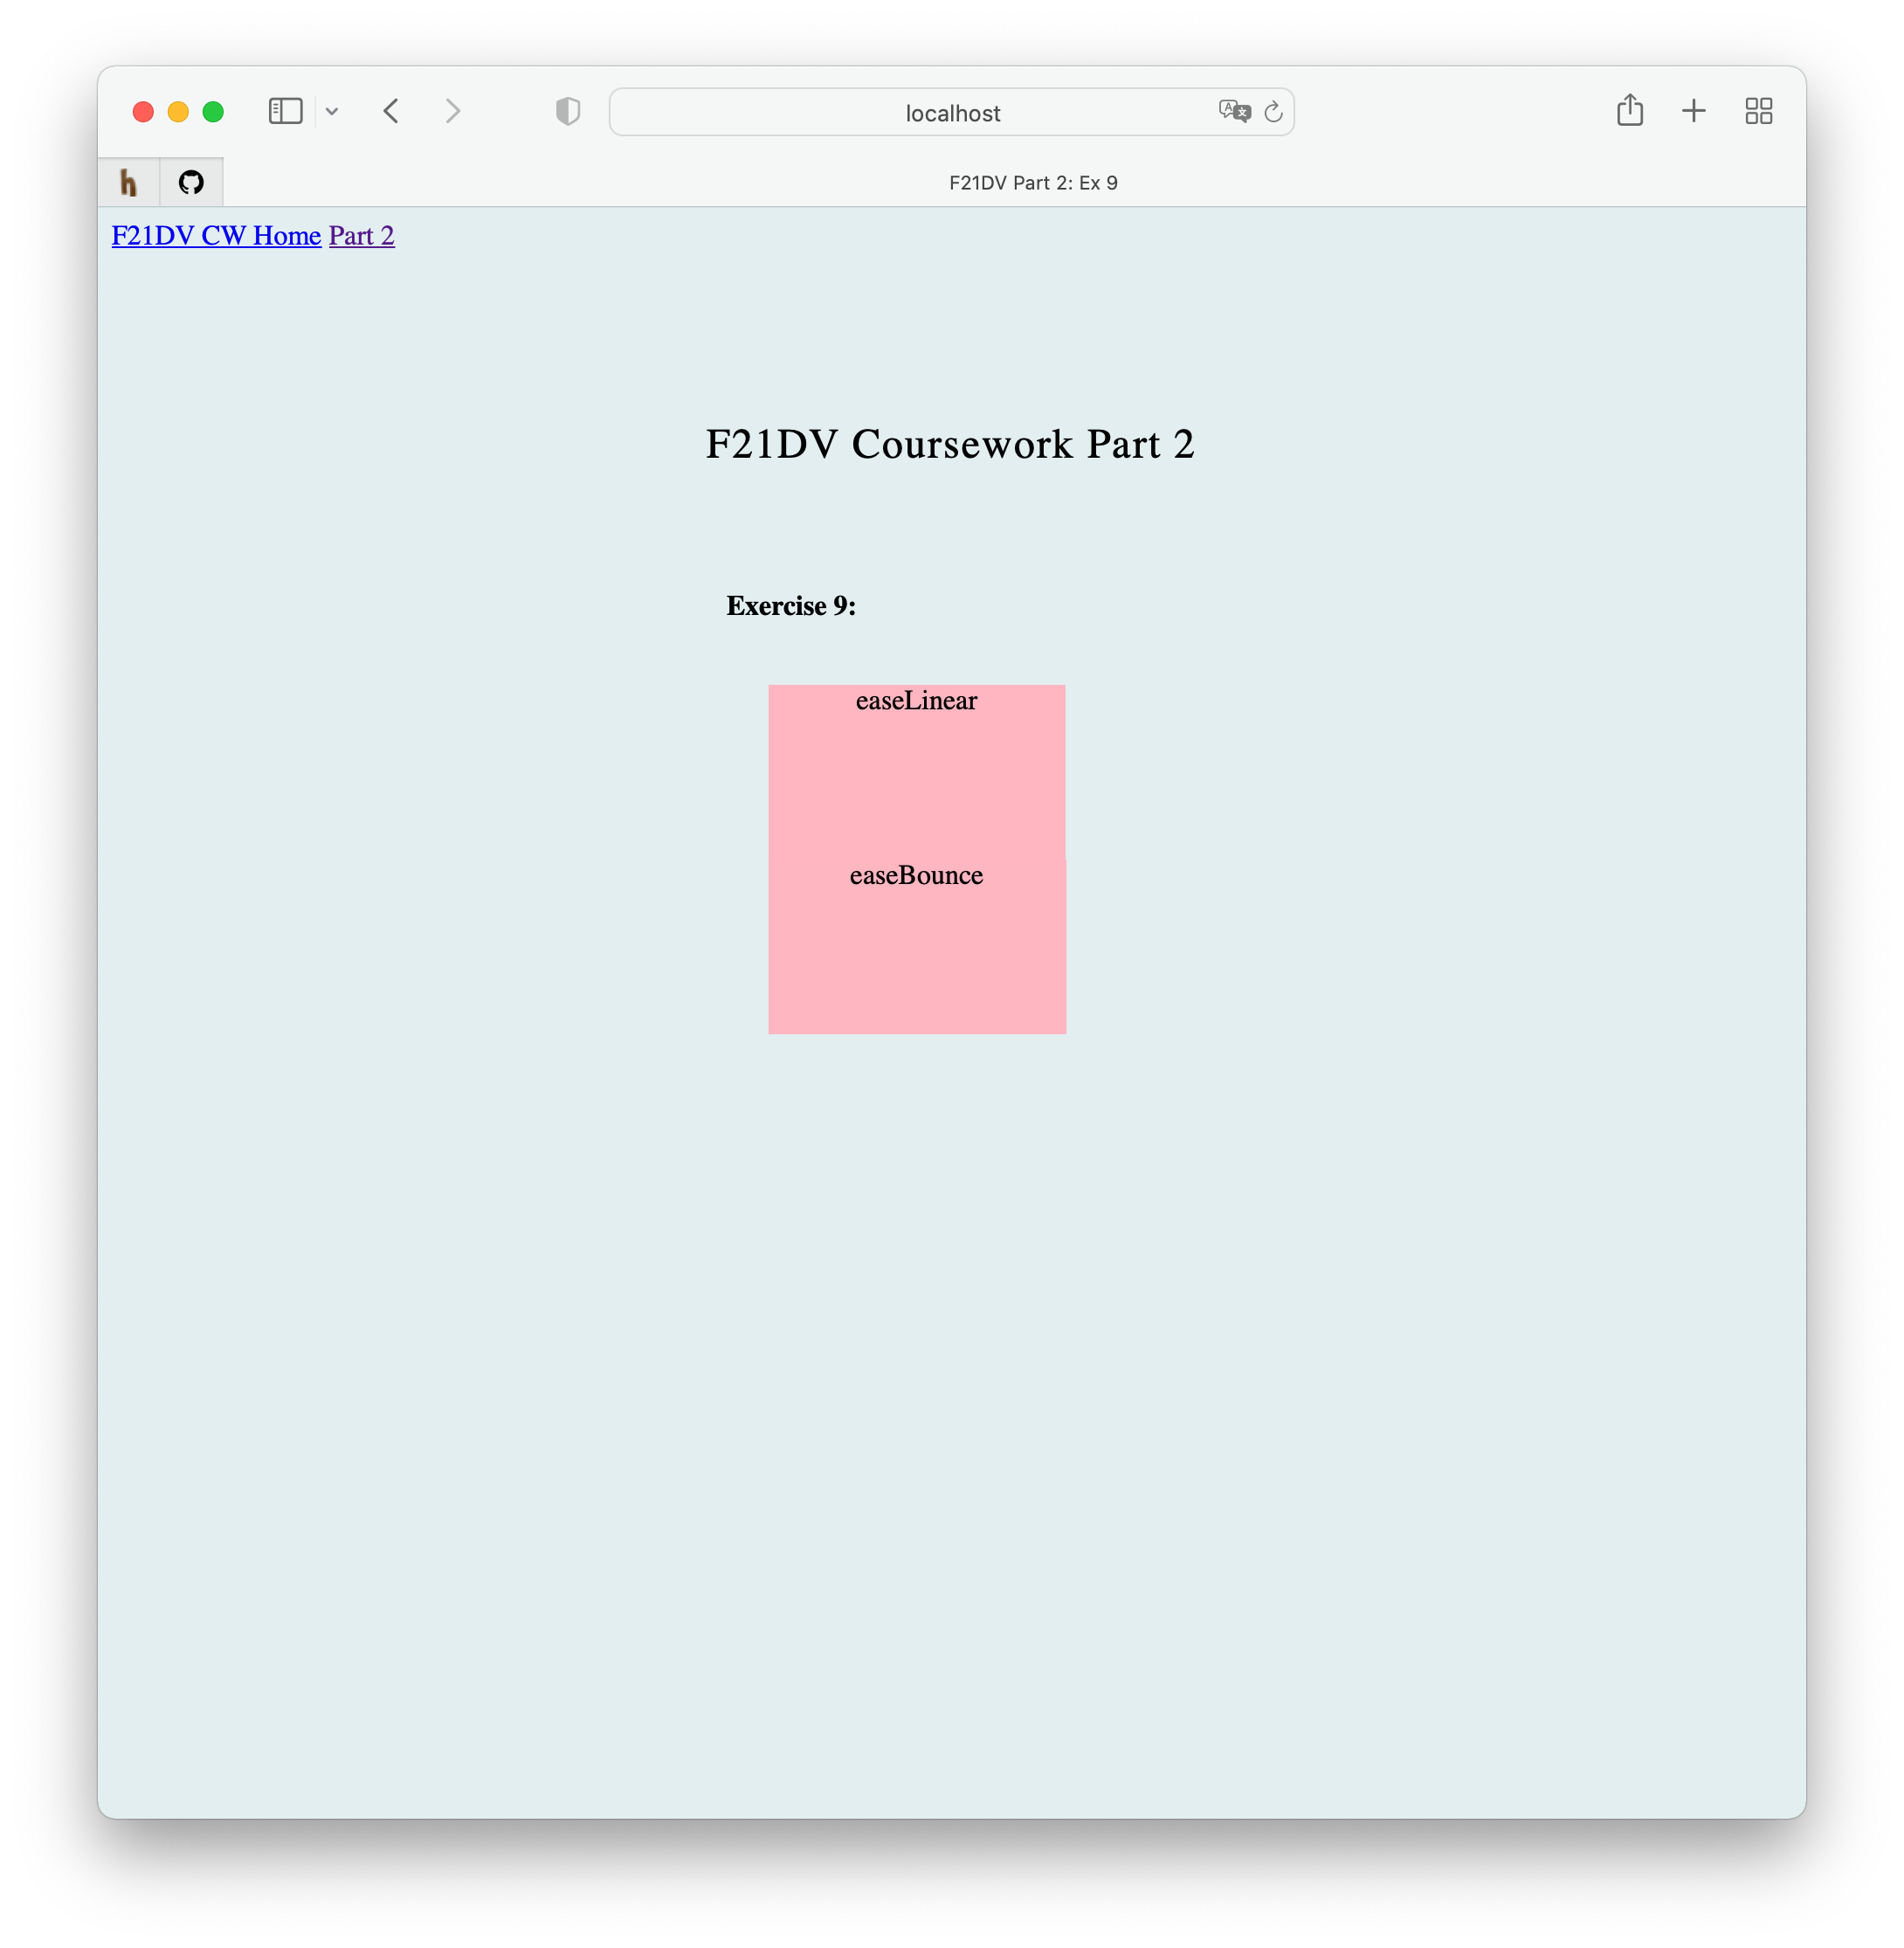
\includegraphics[width = 7.5cm]{images/ex9_3.png}
    \label{fig:ex12}
    \caption{Exercise 12}
\end{figure}
\FloatBarrier
% \lstinputlisting[language=JavaScript]{../../public/js/part2/task12.js}
Figure \ref{fig:ex12} shows an svg annimation that works on load. On load, three bars of different sizes start would start to form, one after another. This transition starts on page load. The transition between each block is being delayed so that they start one after another.

\newpage
\section{Exercise 13}
\begin{figure}[!ht]
    \centering
    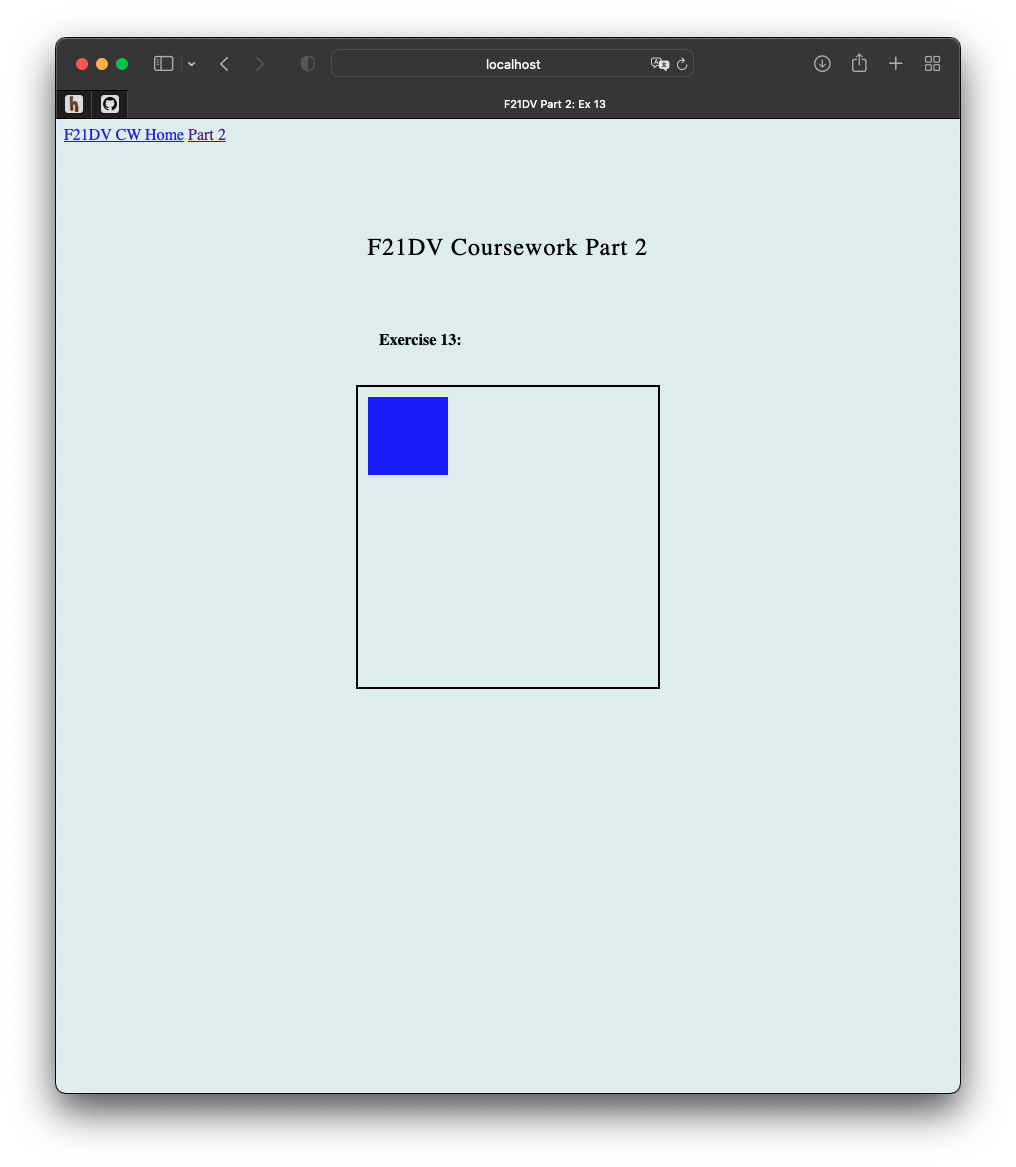
\includegraphics[width = 7.5cm]{images/ex13_1.png}
    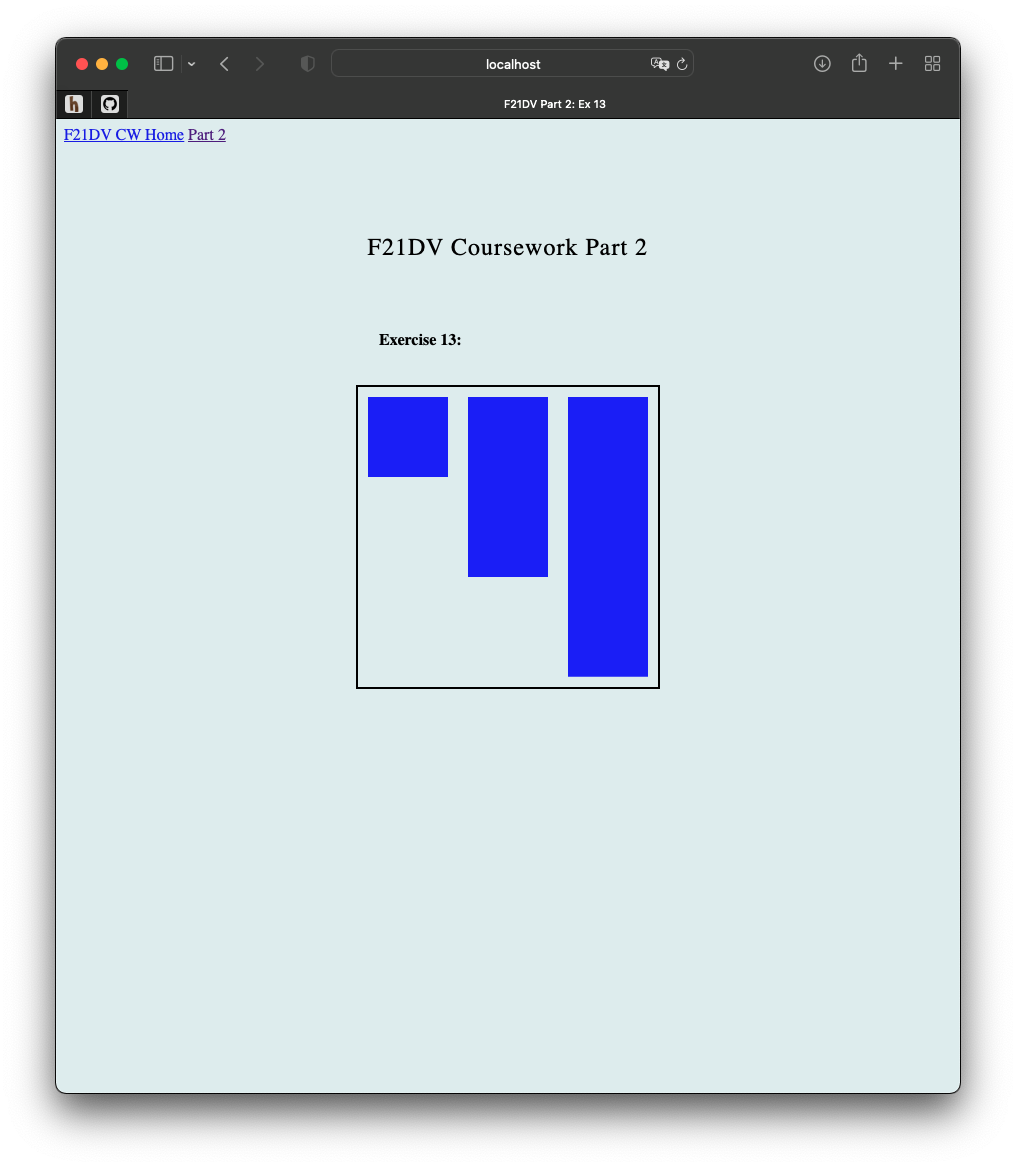
\includegraphics[width = 7.5cm]{images/ex13_2.png}
    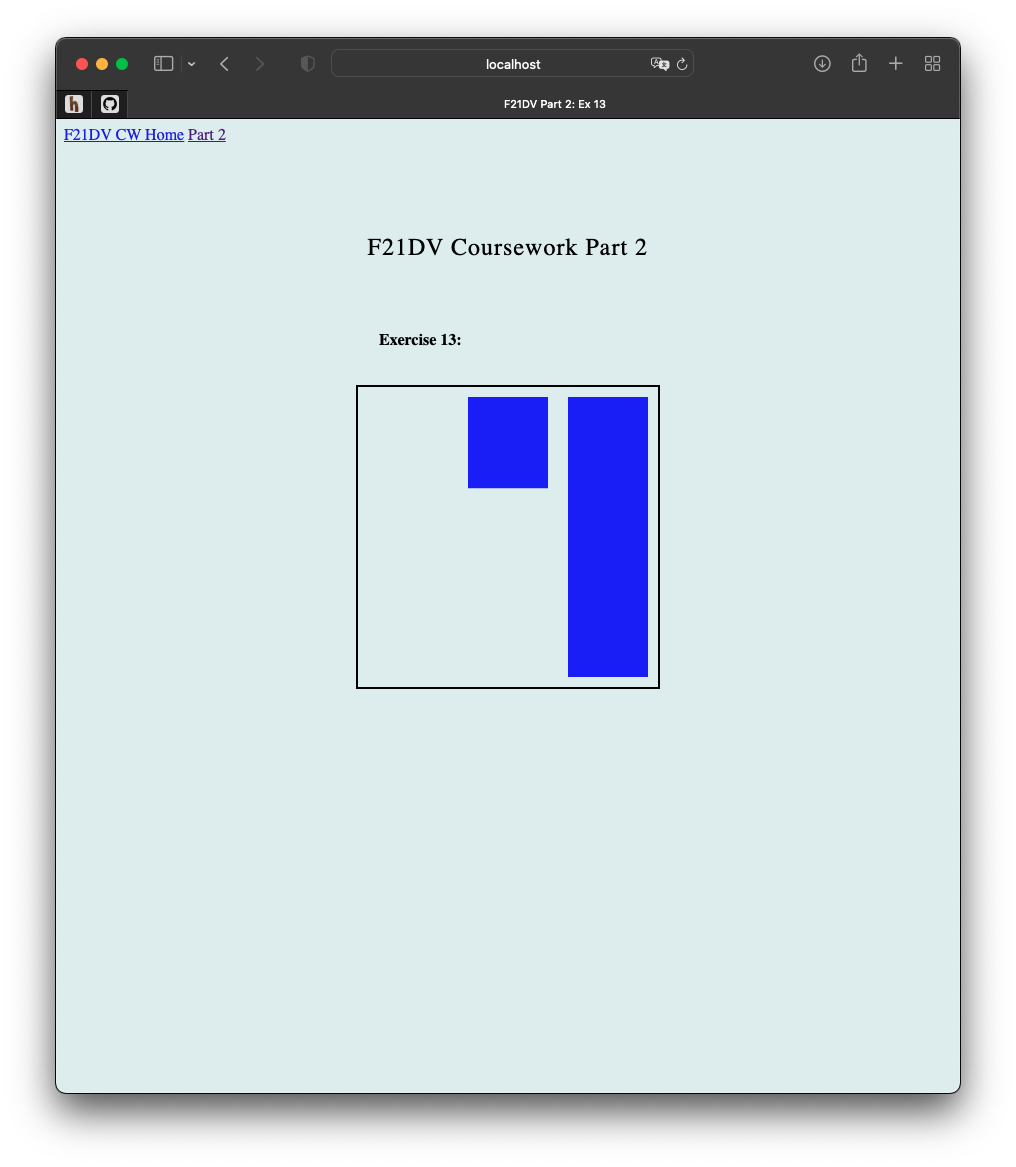
\includegraphics[width = 7.5cm]{images/ex13_3.png}
    \label{fig:ex13}
    \caption{Exercise 13}
\end{figure}
\FloatBarrier
% \lstinputlisting[language=JavaScript]{../../public/js/part2/task12.js}
Figure \ref{fig:ex13} shows the same svg animation as the one in exercise 12. This time, the annimation would annimate out just like the figure above, in the same sequence and the starting annimation.

\newpage
\section{Exercise 14}
\begin{figure}[!ht]
    \centering
    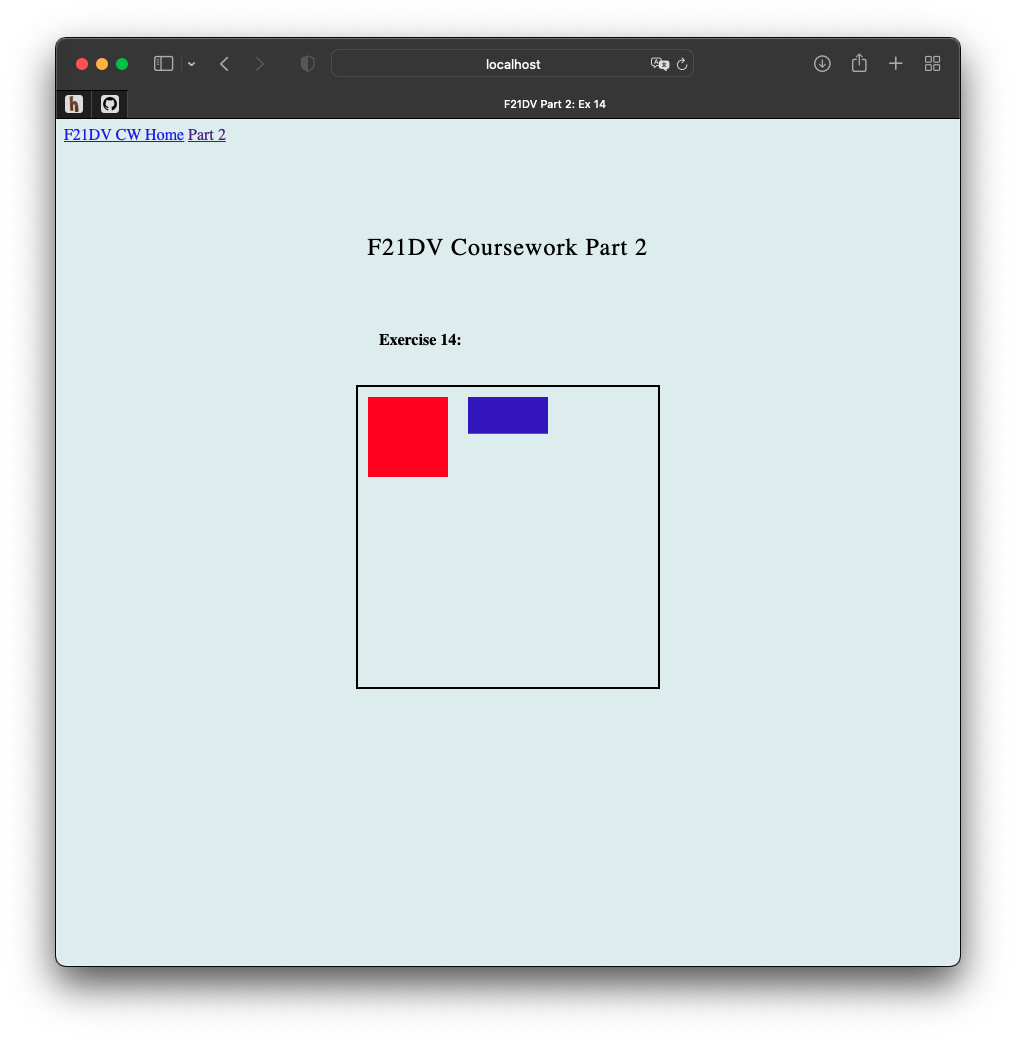
\includegraphics[width = 7.5cm]{images/ex14_1.png}
    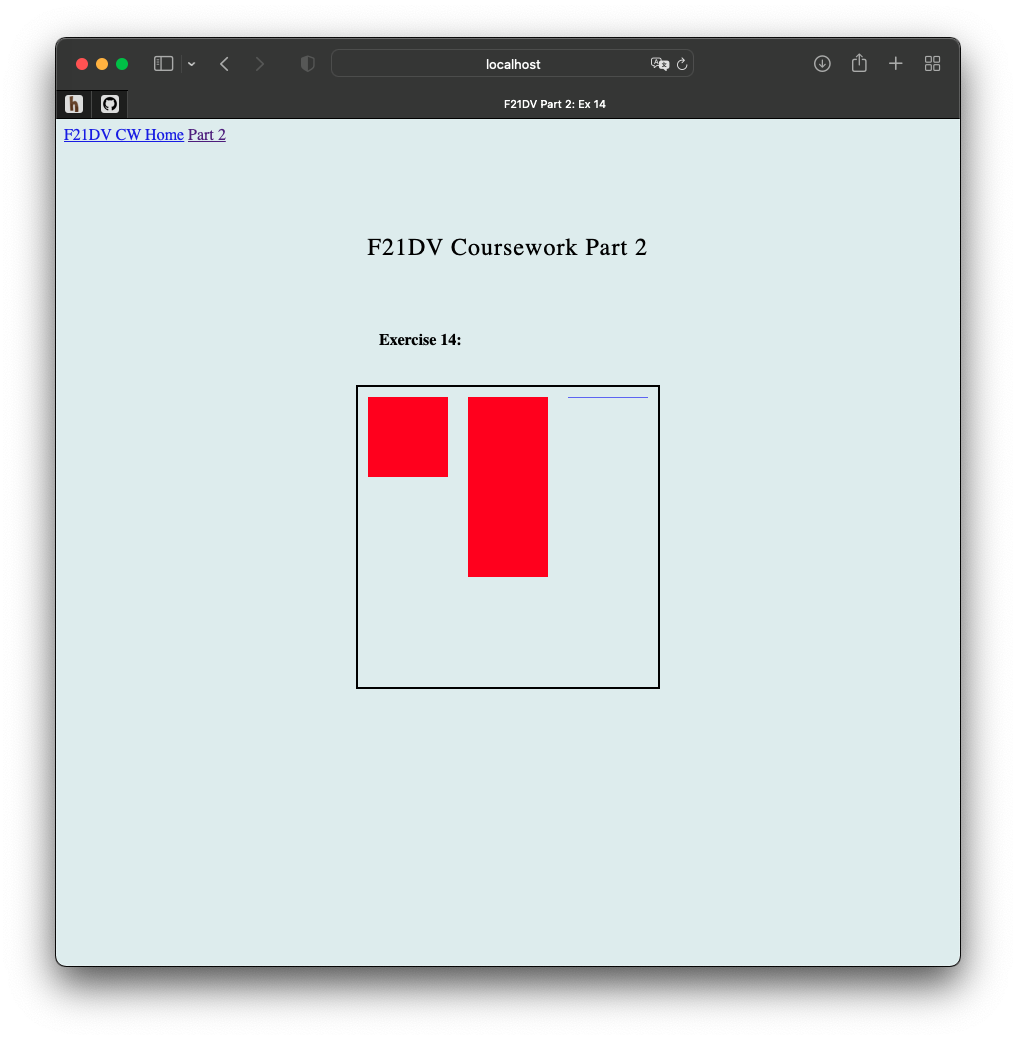
\includegraphics[width = 7.5cm]{images/ex14_2.png}
    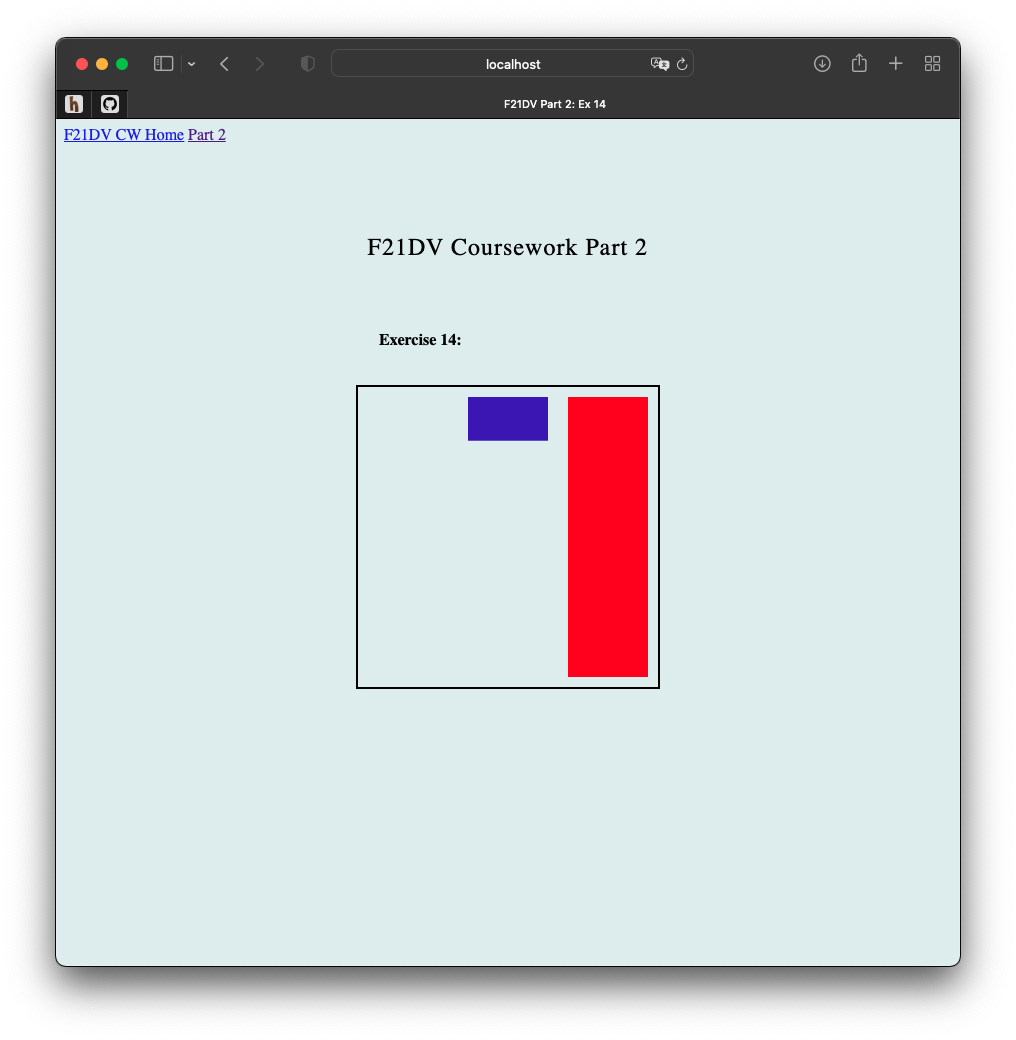
\includegraphics[width = 7.5cm]{images/ex14_3.png}
    \label{fig:ex14}
    \caption{Exercise 14}
\end{figure}
\FloatBarrier
% \lstinputlisting[language=JavaScript]{../../public/js/part2/task12.js}
Figure \ref{fig:ex14} shows the same svg animation as the one in exercise 13. THe difference is that now the annimation would change from blue to red upon the start annimation, and would change from red back to blue for the eciting annimation.

\newpage
\section{Exercise 15}
\begin{figure}[!ht]
    \centering
    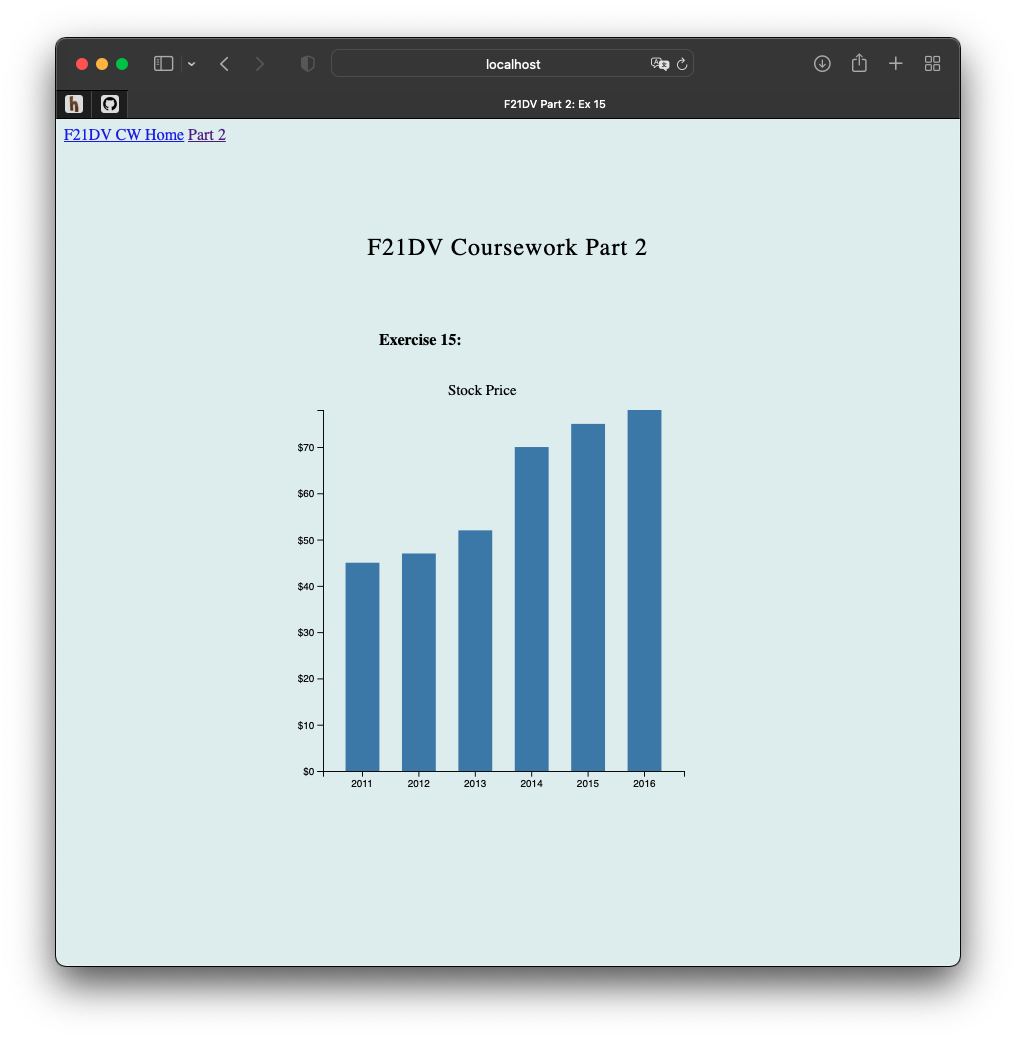
\includegraphics[width = 7.5cm]{images/ex15_1.png}
    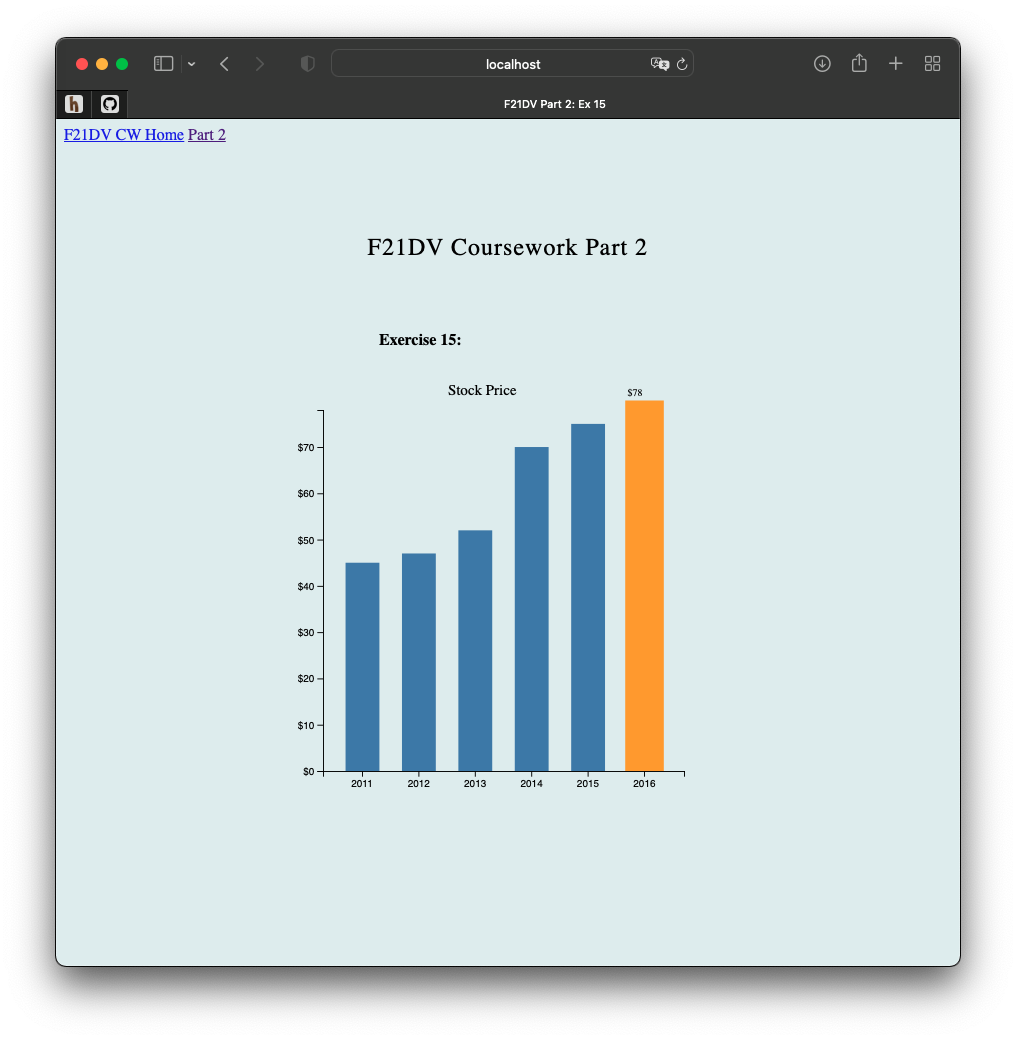
\includegraphics[width = 7.5cm]{images/ex15_2.png}
    % 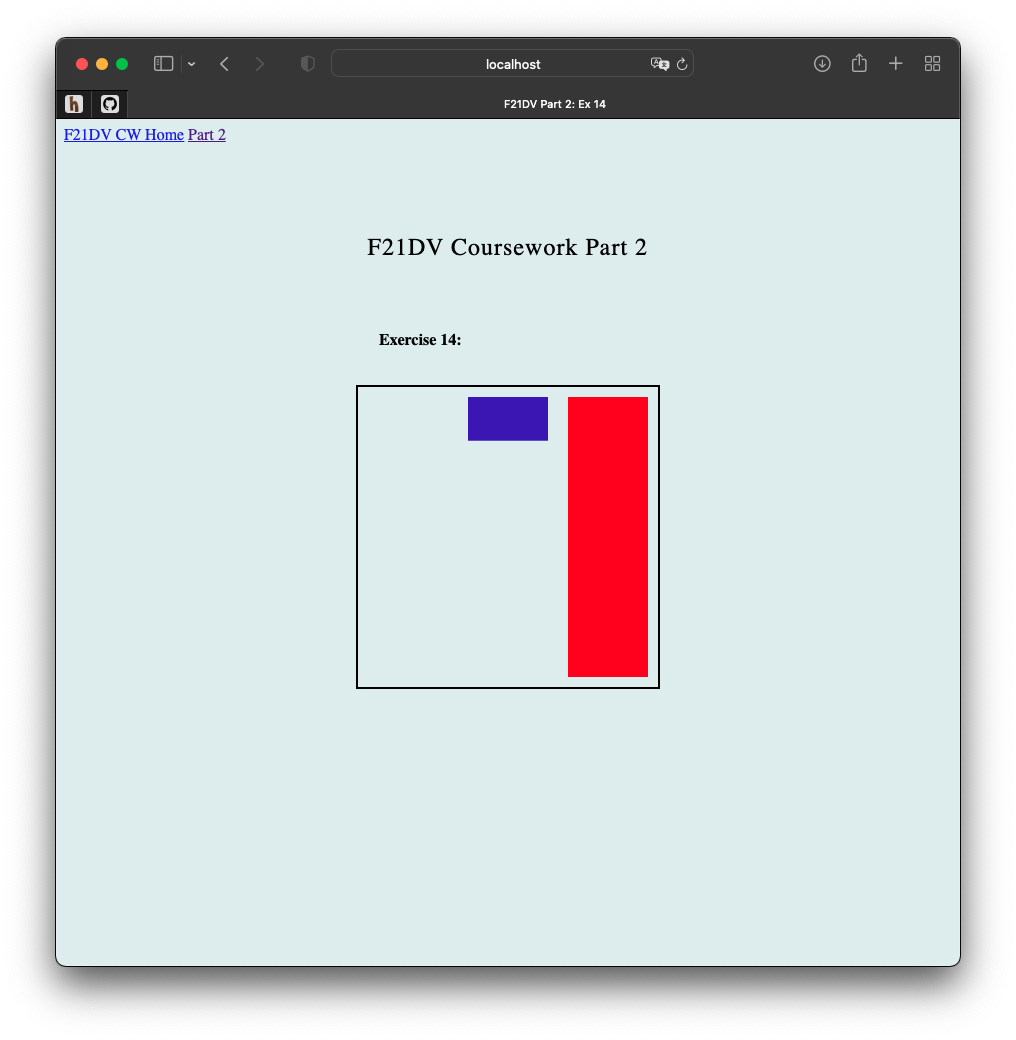
\includegraphics[width = 7.5cm]{images/ex14_3.png}
    \label{fig:ex15}
    \caption{Exercise 15}
\end{figure}
\FloatBarrier
% \lstinputlisting[language=JavaScript]{../../public/js/part2/task12.js}
Figure \ref{fig:ex15} shows a bar chart upon load. Upon hover of a specific bar chart, the bar chart would enlarge itself, and show its actual y-axis value (price of stock) on top of the bar.

\newpage
\section{Exercise 16}
\begin{figure}[!ht]
    \centering
    % 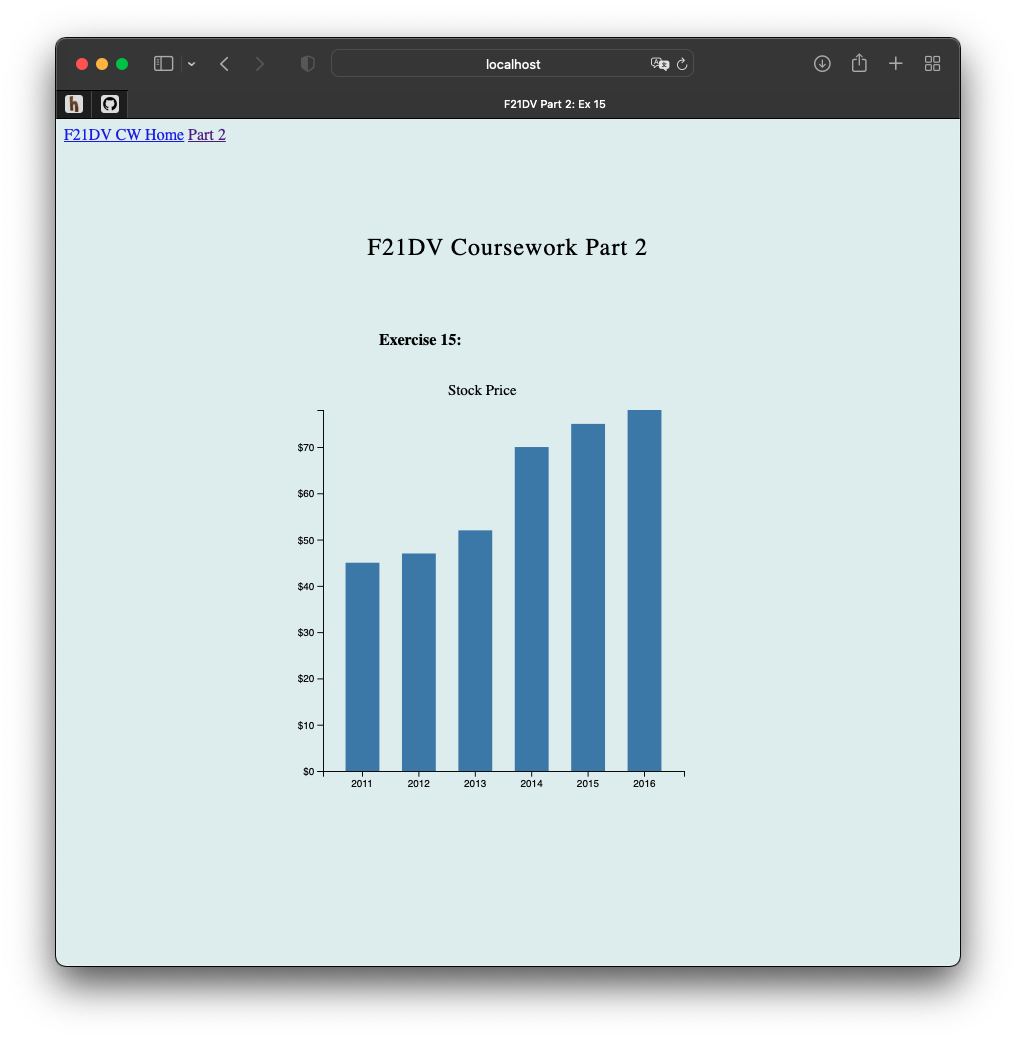
\includegraphics[width = 7.5cm]{images/ex15_1.png}
    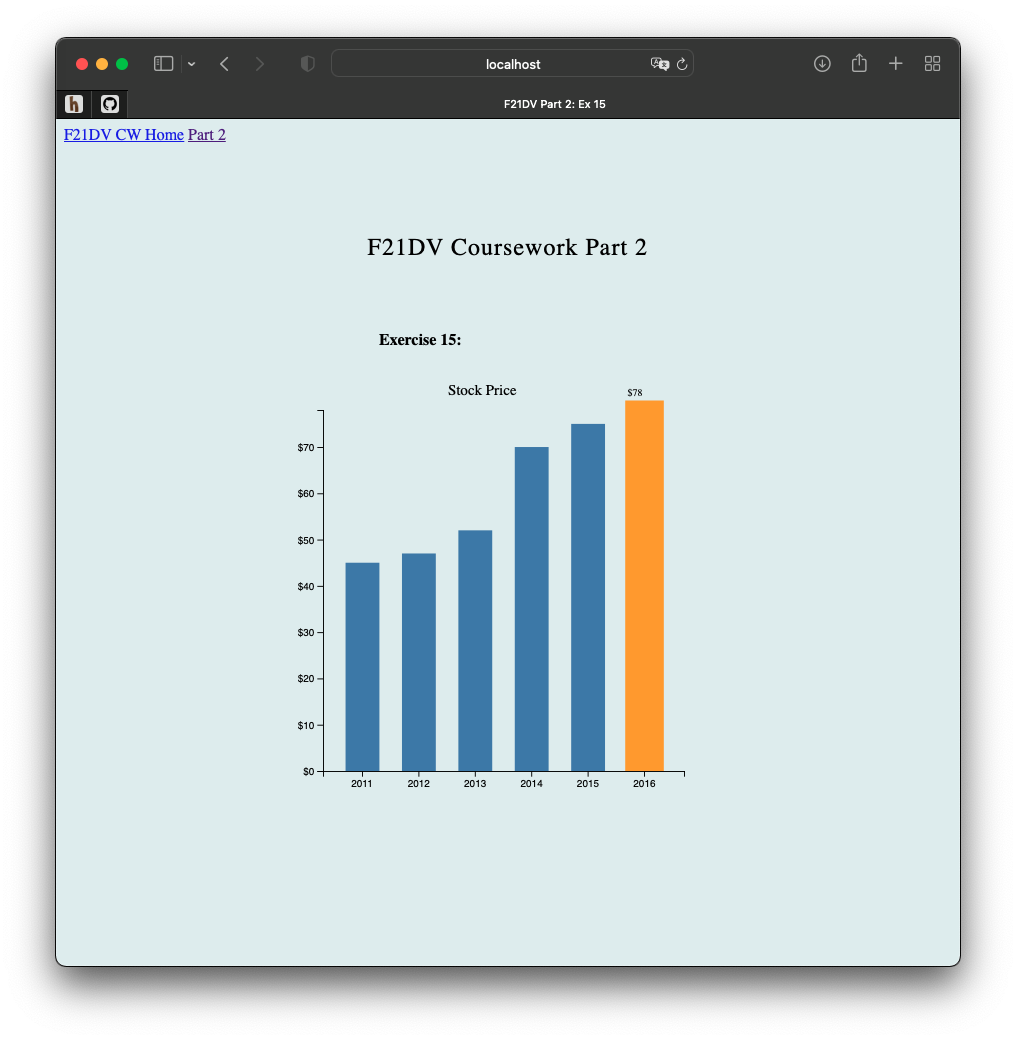
\includegraphics[width = 7.5cm]{images/ex15_2.png}
    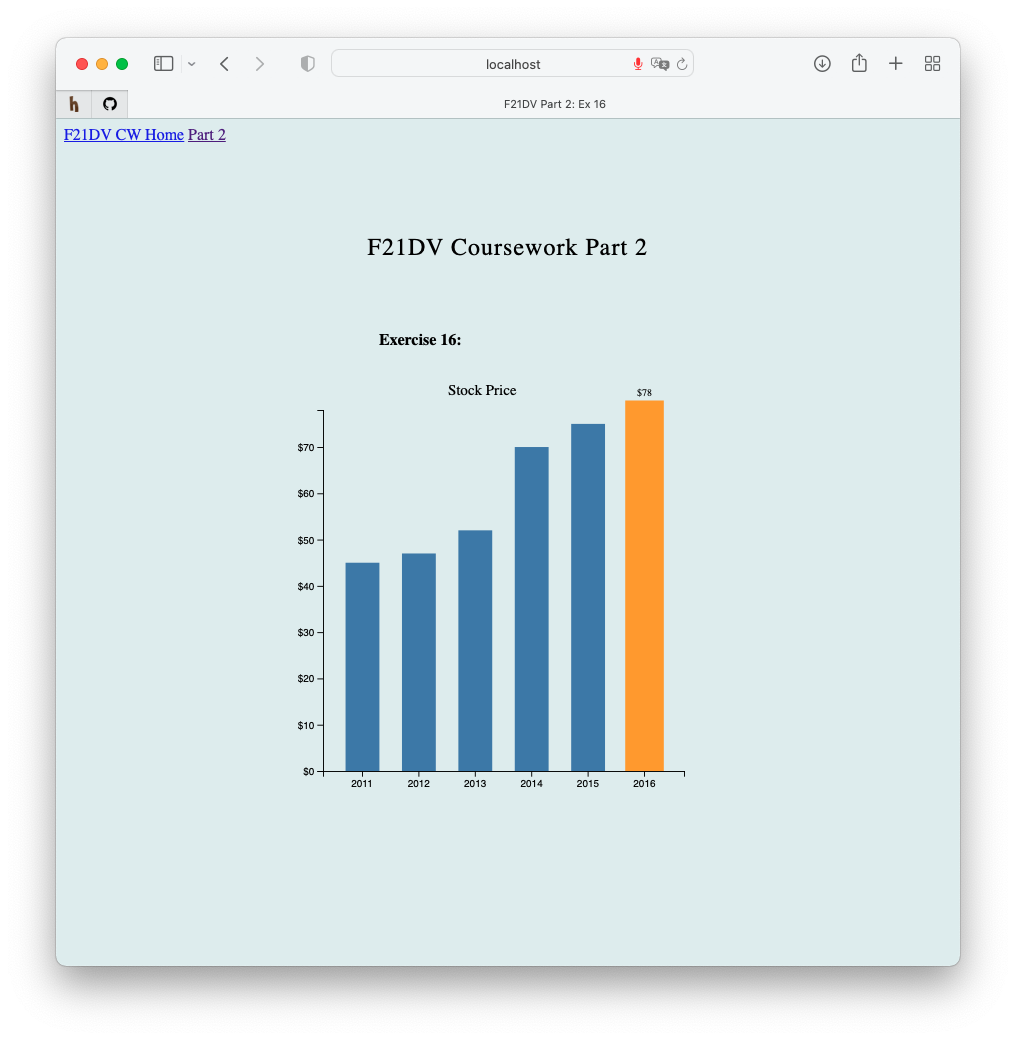
\includegraphics[width = 7.5cm]{images/ex16.png}
    \label{fig:ex16}
    \caption{Exercise 16}
\end{figure}
\FloatBarrier
% \lstinputlisting[language=JavaScript]{../../public/js/part2/task12.js}
Figure \ref{fig:ex16} shows a bar chart upon load, asme as the one shown in example 15, figure \ref{fig:ex15}. The difference is that now on hover, the price shown on top of the bar is centered in the middle instead of on the side. 

\newpage
\section{Exercise 17}
\begin{figure}[!ht]
    \centering
    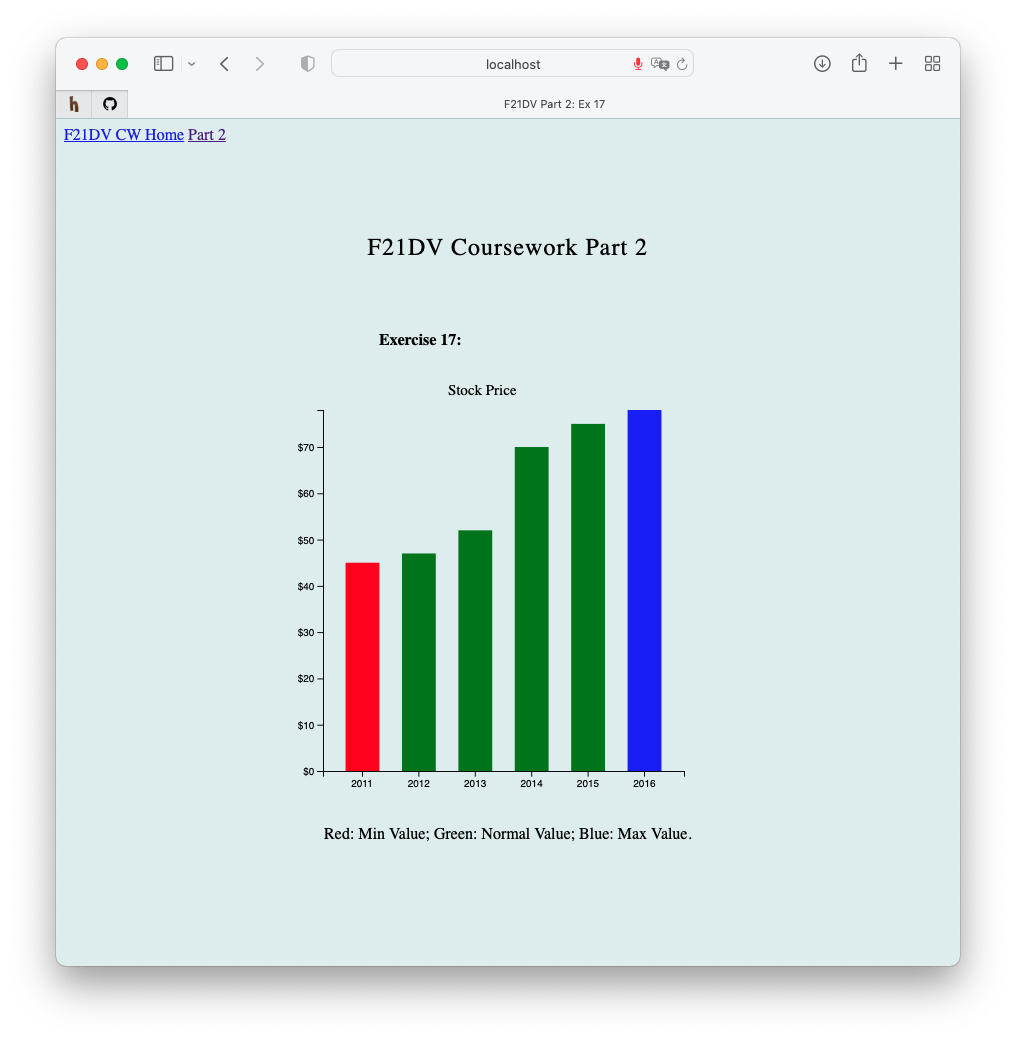
\includegraphics[width = 7.5cm]{images/ex17_1.png}
    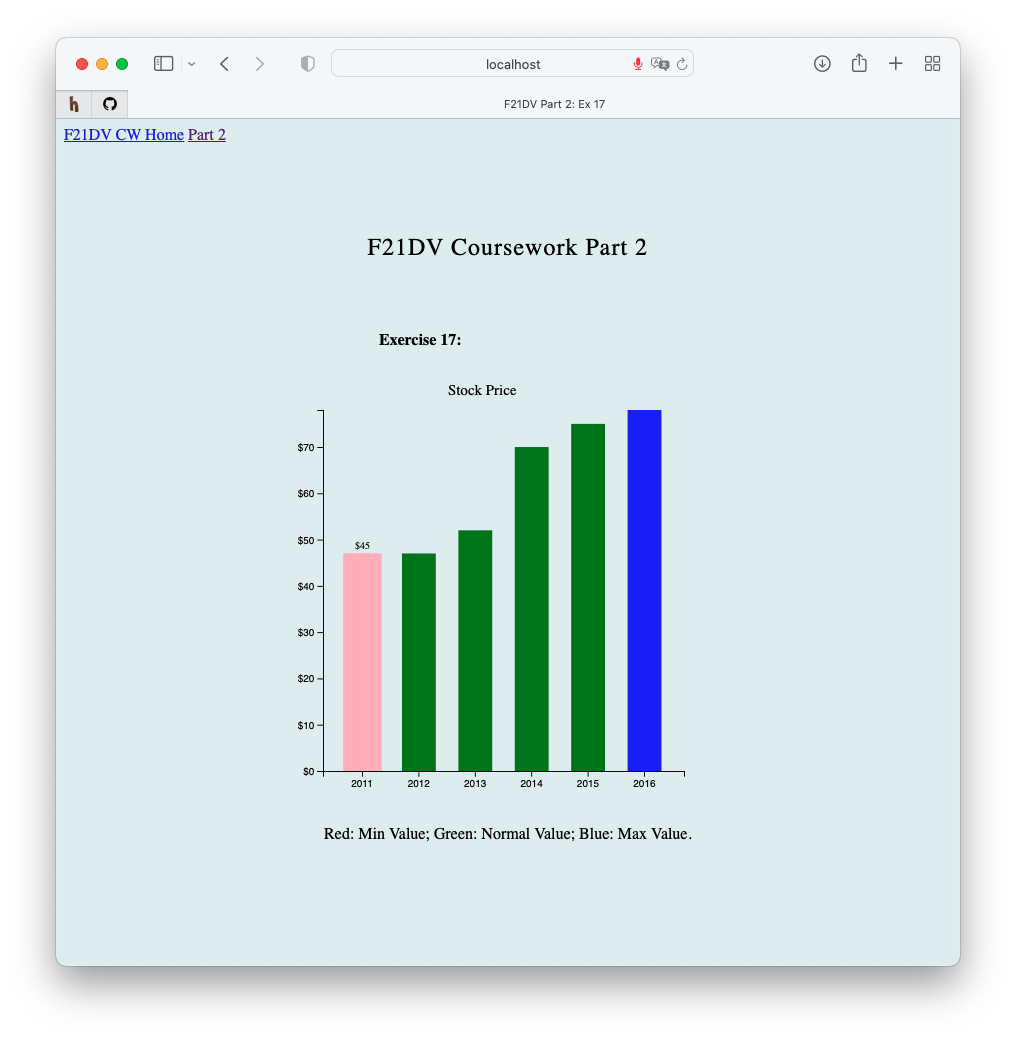
\includegraphics[width = 7.5cm]{images/ex17_2.png}
    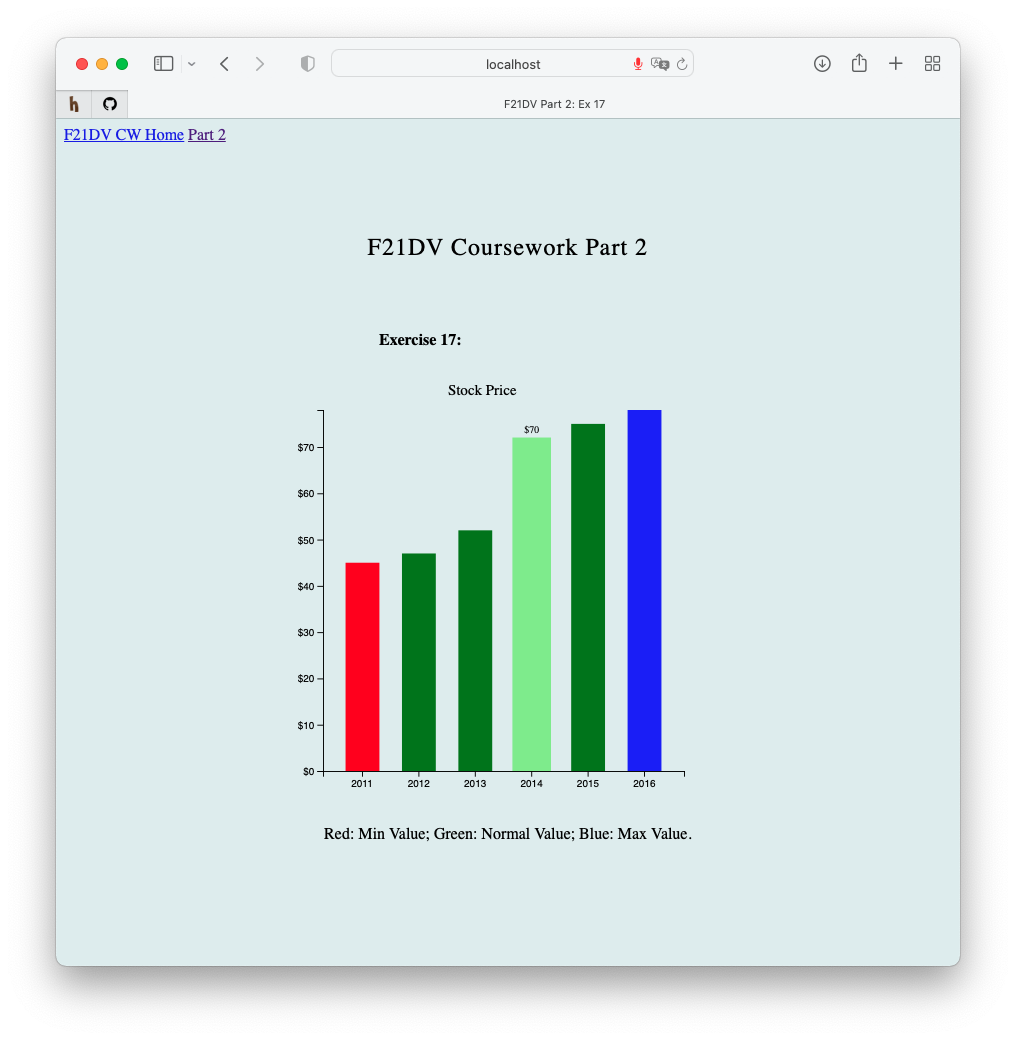
\includegraphics[width = 7.5cm]{images/ex17_3.png}
    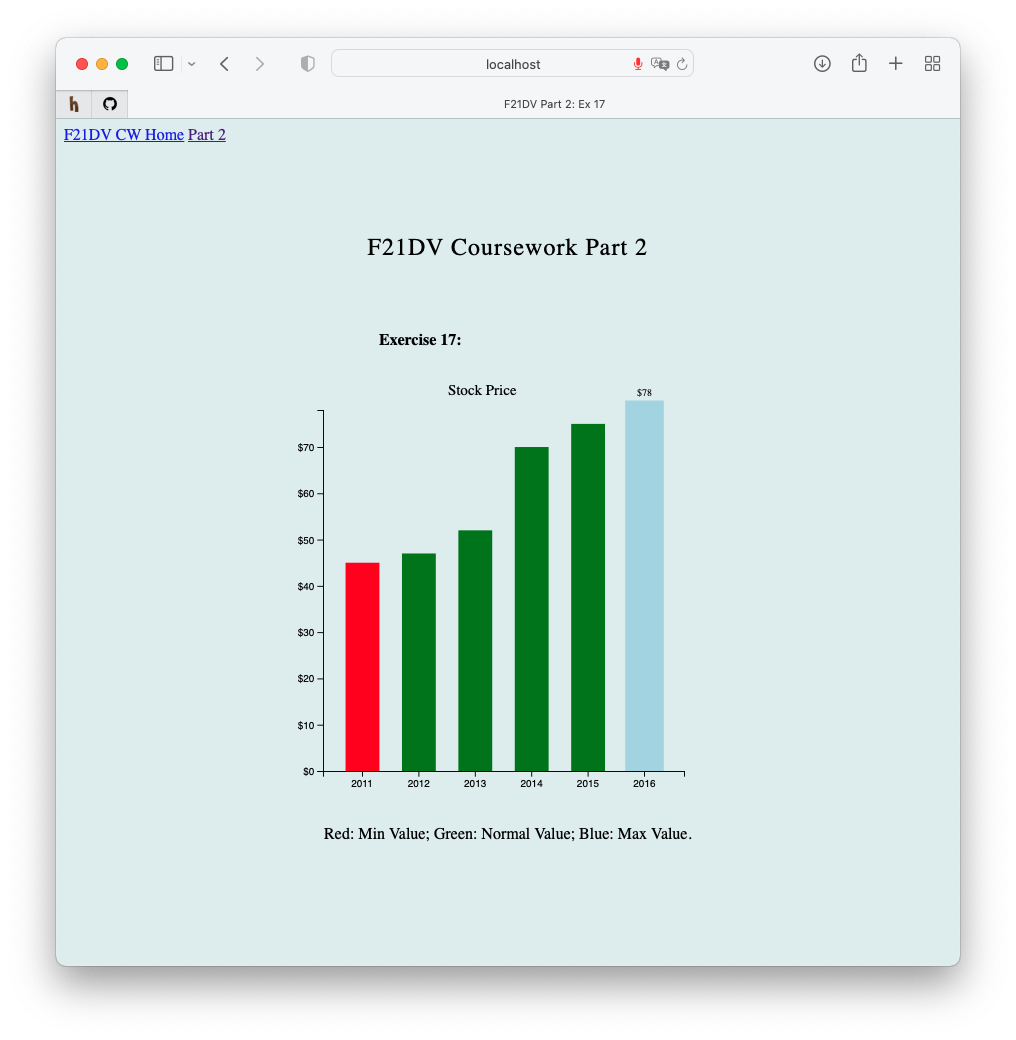
\includegraphics[width = 7.5cm]{images/ex17_4.png}
    \label{fig:ex17}
    \caption{Exercise 17}
\end{figure}
\FloatBarrier
\lstinputlisting[language=JavaScript]{../../public/js/part2/task17.js}
Figure \ref{fig:ex17} shows a bar chart upon load, same as the one shown in example 15 and 16. The difference is that the bars are now colour coded. Upon Hover, the bars would still show a different colour, as shown in the images above.  

\subsection{Explaination for Exercise 15 to 17.}
Exercise 15-17's price tag text is transitioned by adding a \verb|text| item each time on mouse over. And Removed everytime on mouse out.


\newpage
\section{Exercise 18}
\begin{figure}[!ht]
    \centering
    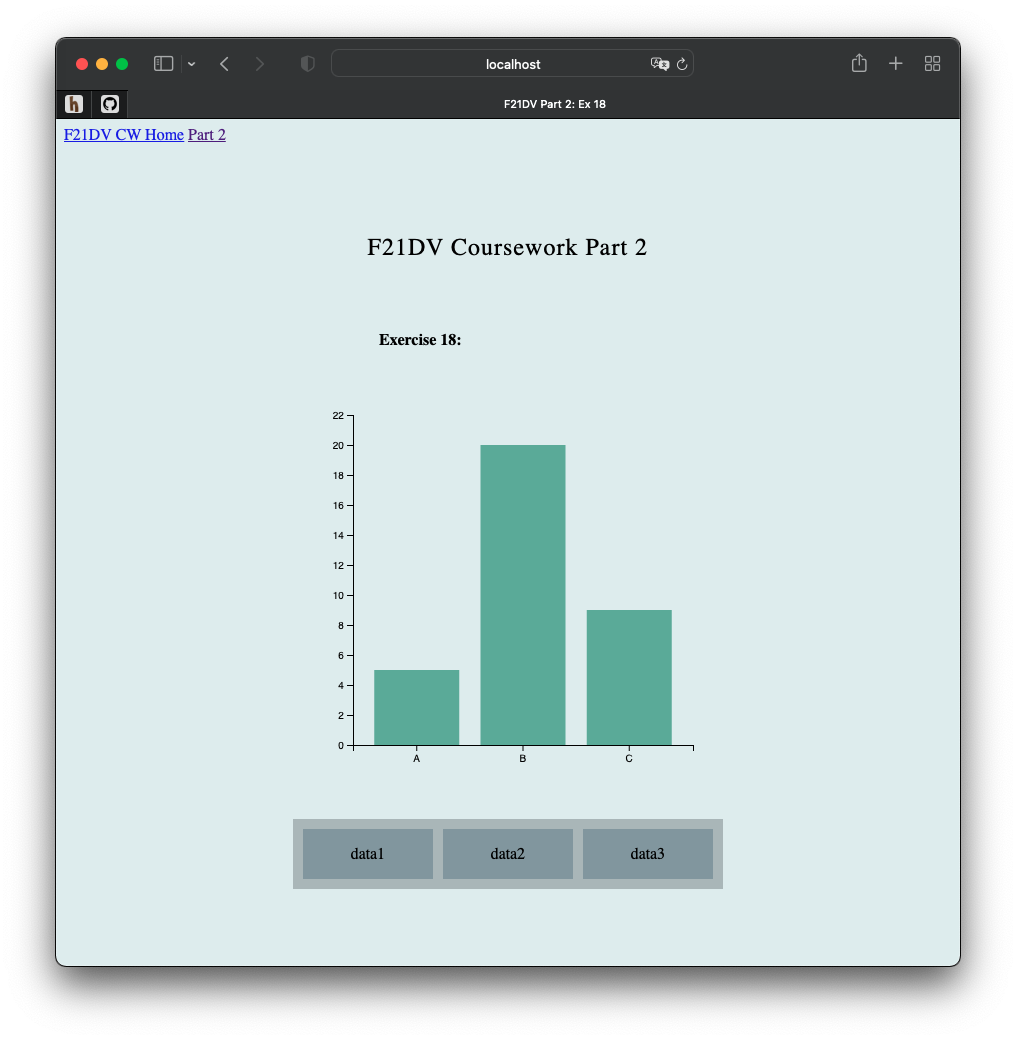
\includegraphics[width = 7.5cm]{images/ex18_1.png}
    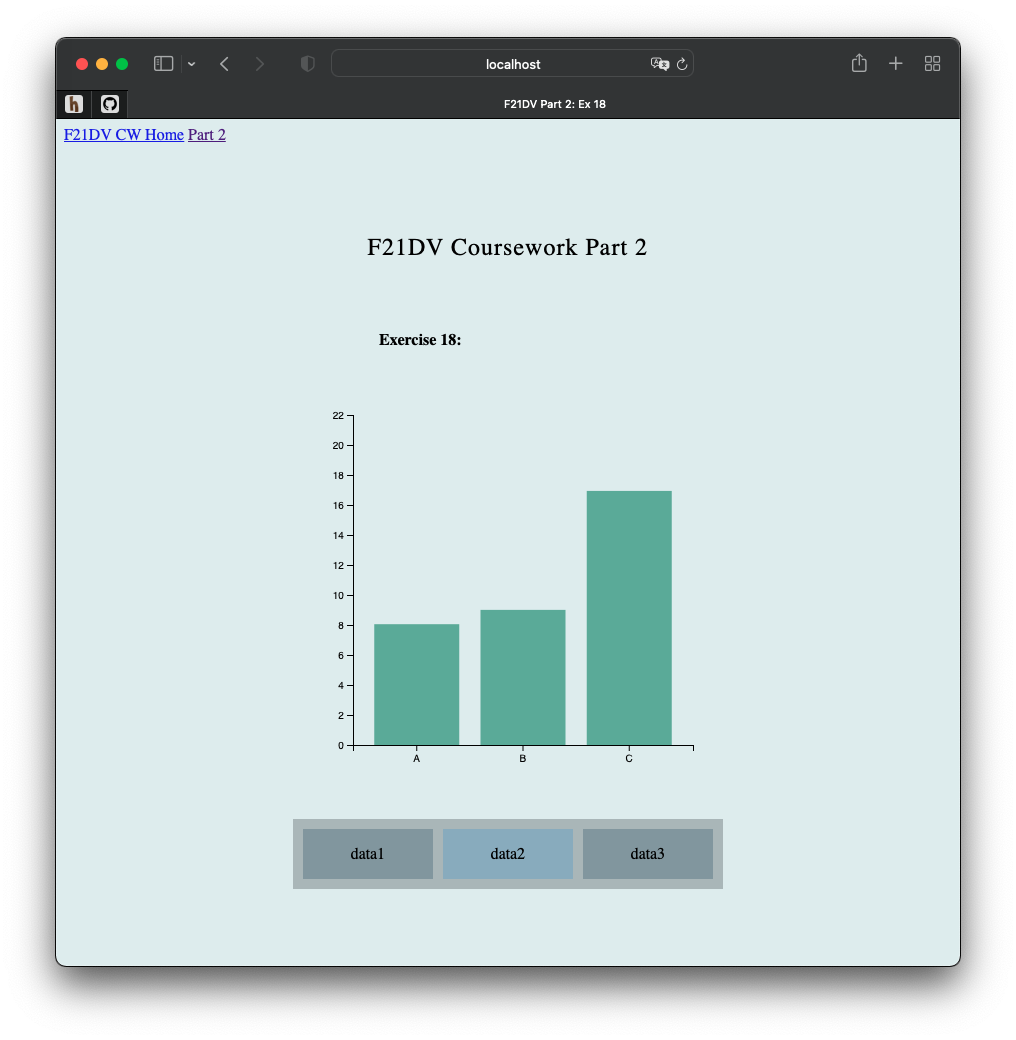
\includegraphics[width = 7.5cm]{images/ex18_2.png}
    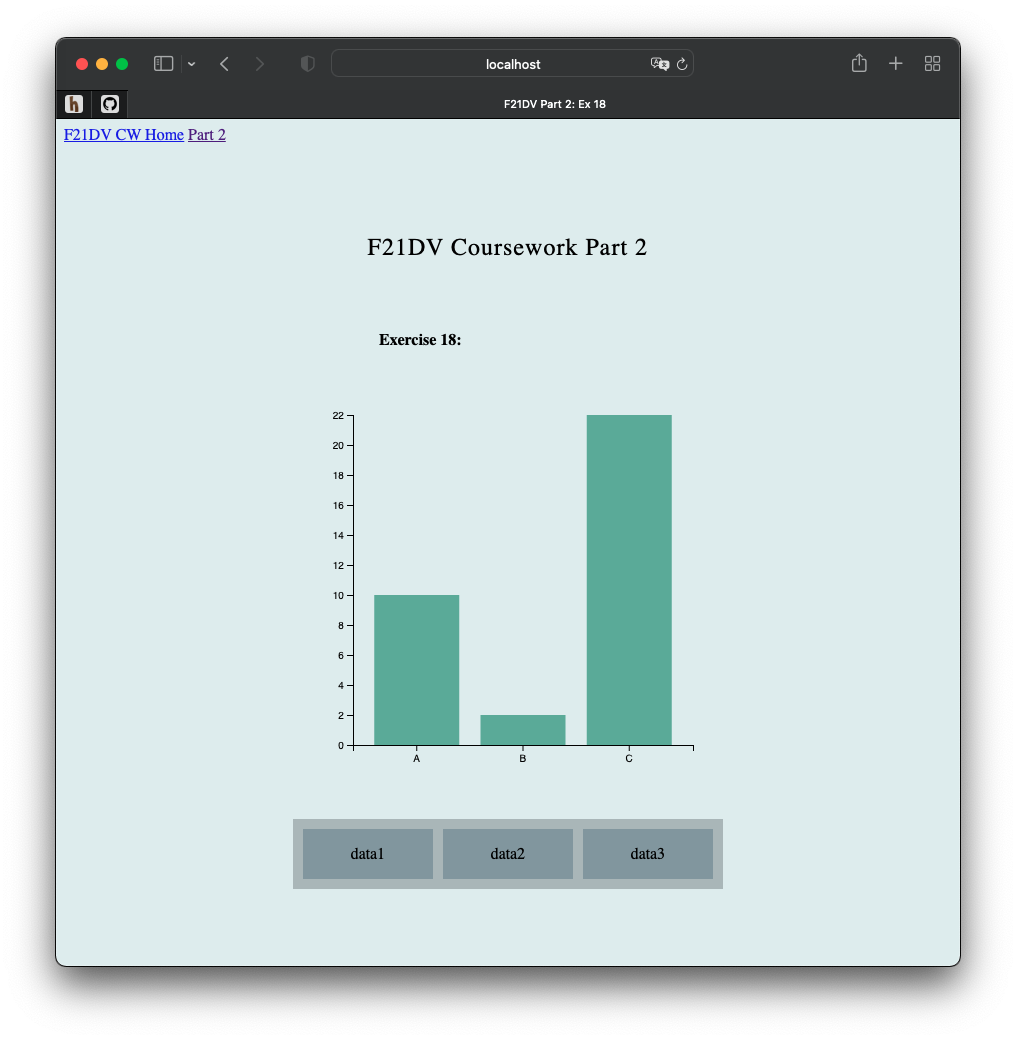
\includegraphics[width = 7.5cm]{images/ex18_3.png}
    % 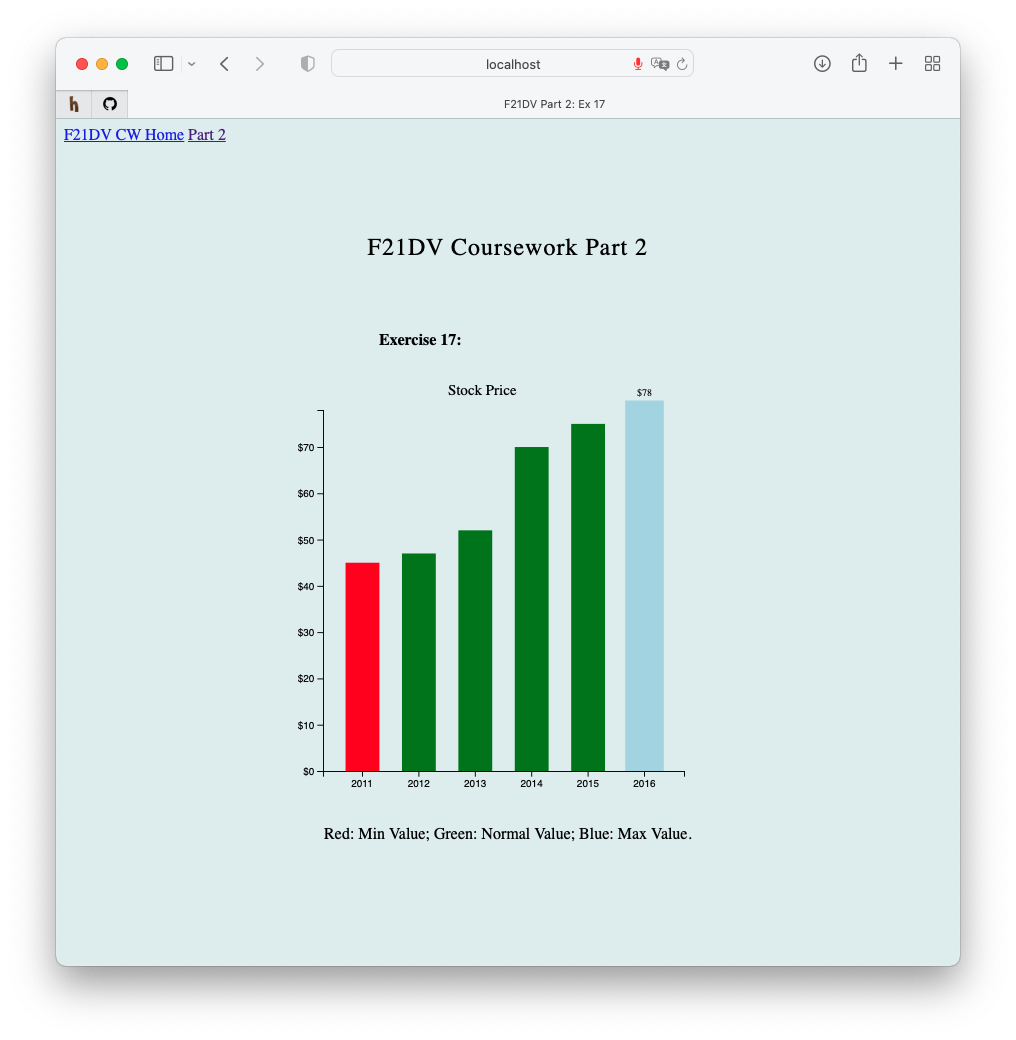
\includegraphics[width = 7.5cm]{images/ex17_4.png}
    \label{fig:ex18}
    \caption{Exercise 18}
\end{figure}
\FloatBarrier
\lstinputlisting[language=JavaScript]{../../public/js/part2/task18.js}
Figure \ref{fig:ex18} shows a bar chart that transitions into a start position showing data 1 upon load. Upon clicking on ``Data 2'', each bar would transition to the new position as shown in the 3-part image above. This is done by using the \verb|.merge()| function as shown.

\newpage
\section{Exercise 19}
\begin{figure}[!ht]
    \centering
    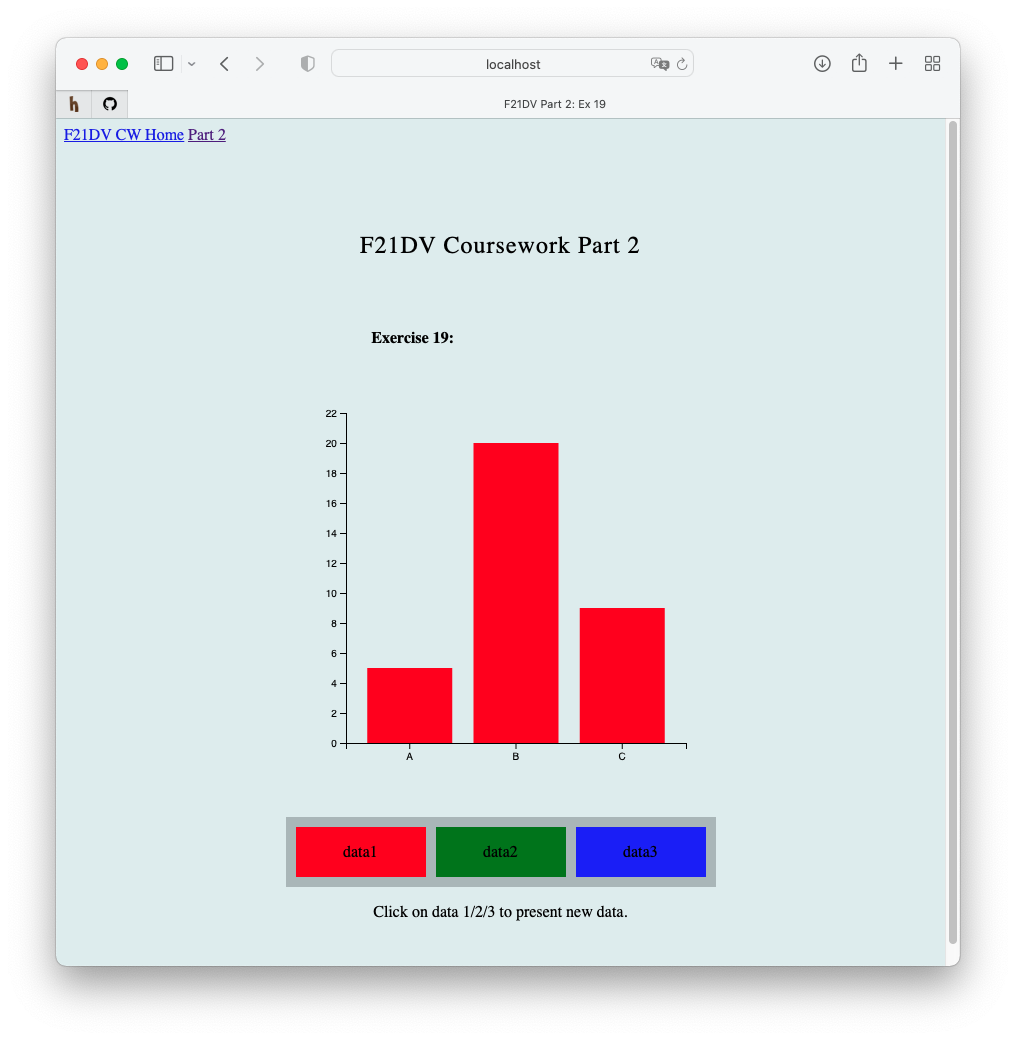
\includegraphics[width = 7.5cm]{images/ex19.png}
    % 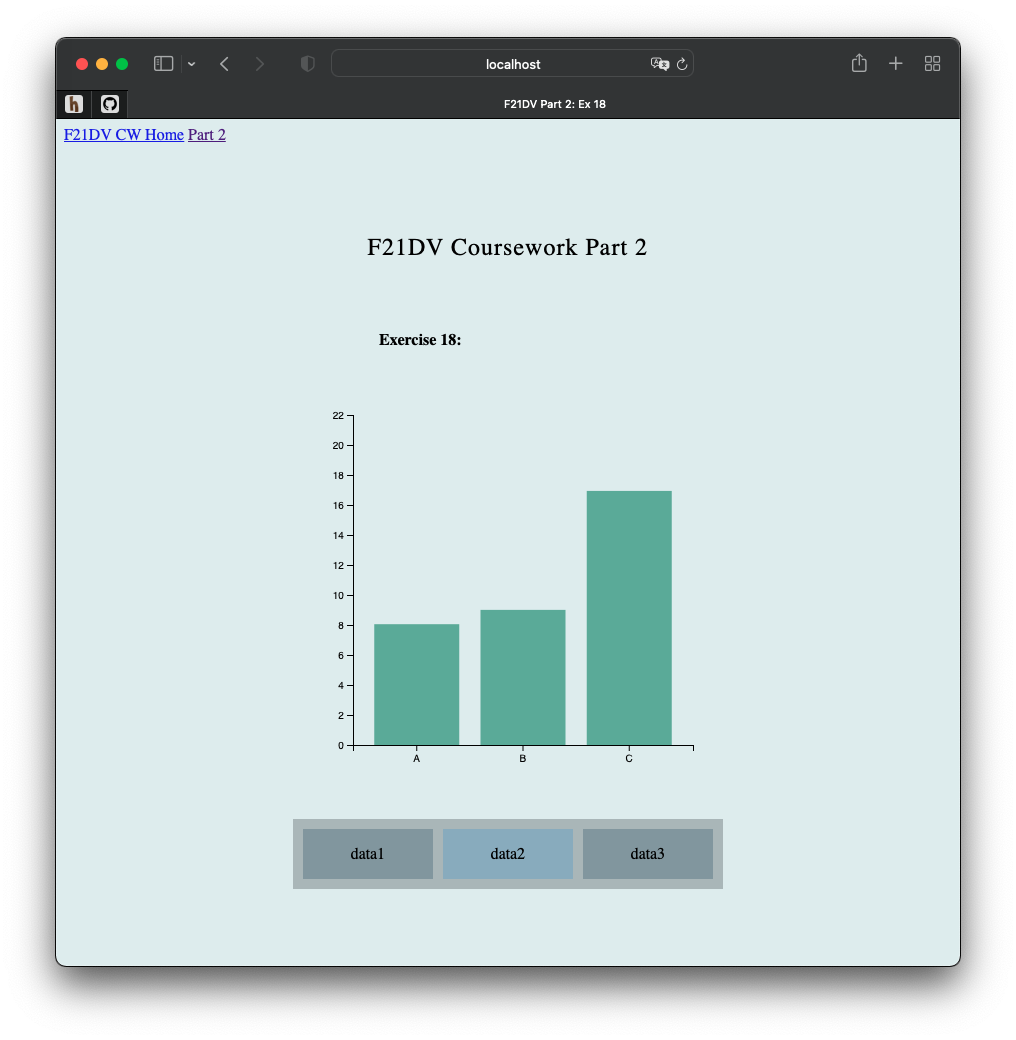
\includegraphics[width = 7.5cm]{images/ex18_2.png}
    % 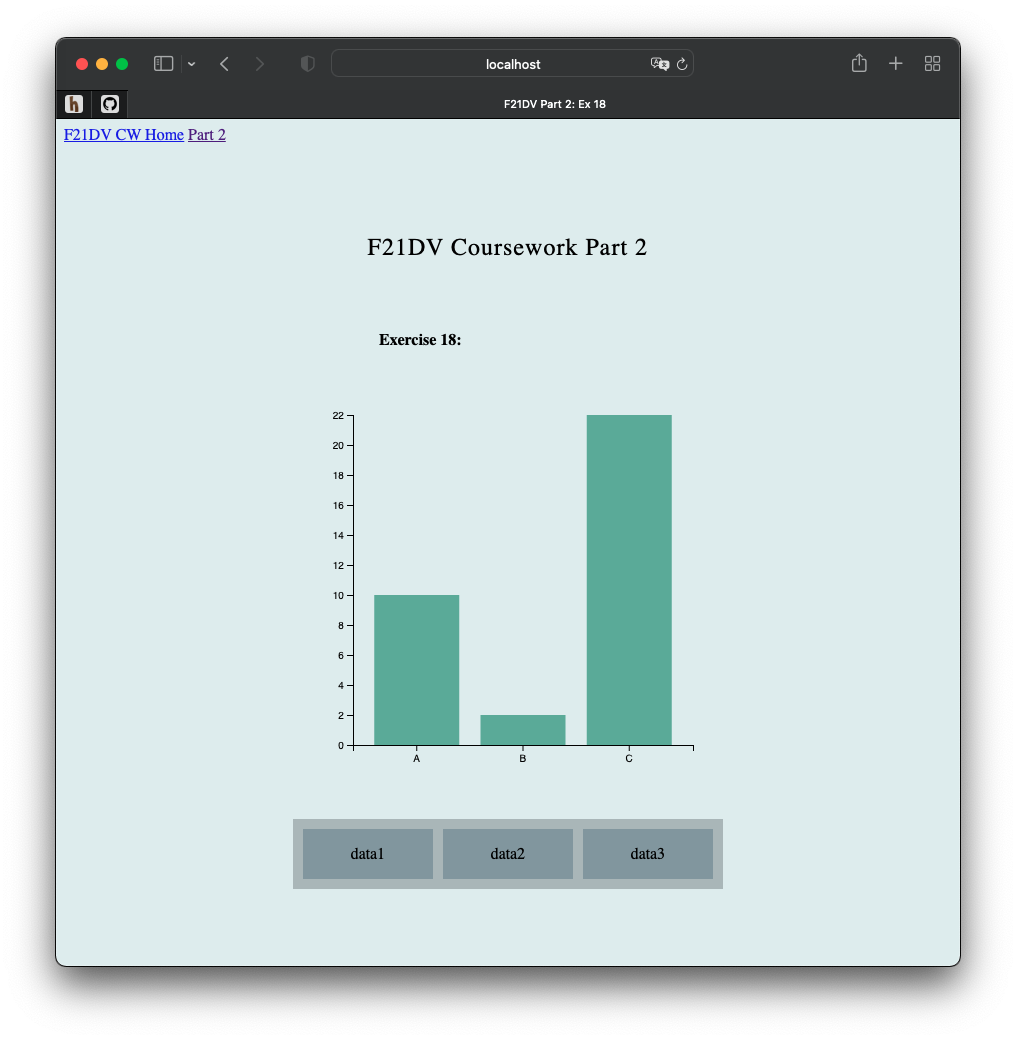
\includegraphics[width = 7.5cm]{images/ex18_3.png}
    % 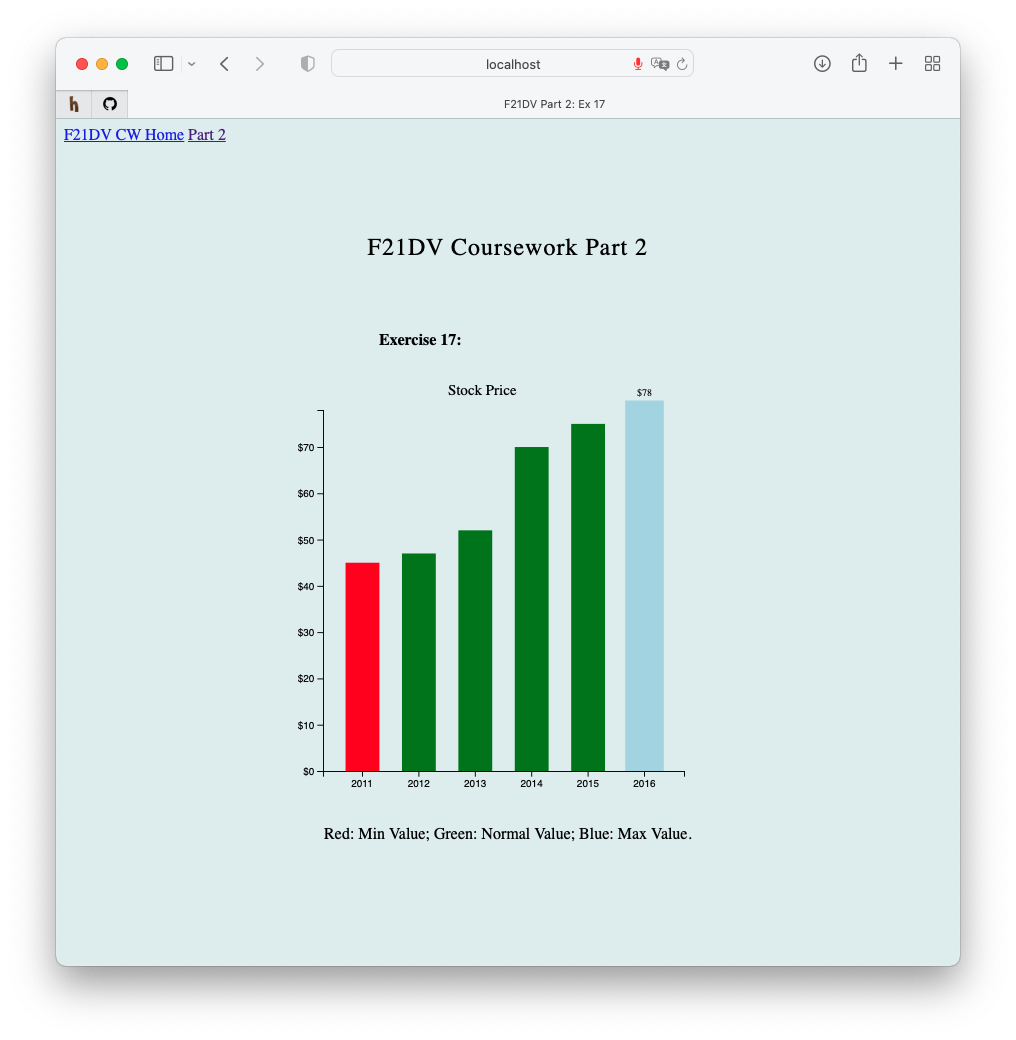
\includegraphics[width = 7.5cm]{images/ex17_4.png}
    \label{fig:ex19}
    \caption{Exercise 19}
\end{figure}
\FloatBarrier
% \lstinputlisting[language=JavaScript]{../../public/js/part2/task18.js}
Figure \ref{fig:ex19} shows the same bar chart as the one on exercise 18. The only difference is that now each data has its own colour. Transitions are still the same, just that now an extra `color' attribute is being added into the transitions.

\newpage
\section{Exercise 20}
\begin{figure}[!ht]
    \centering
    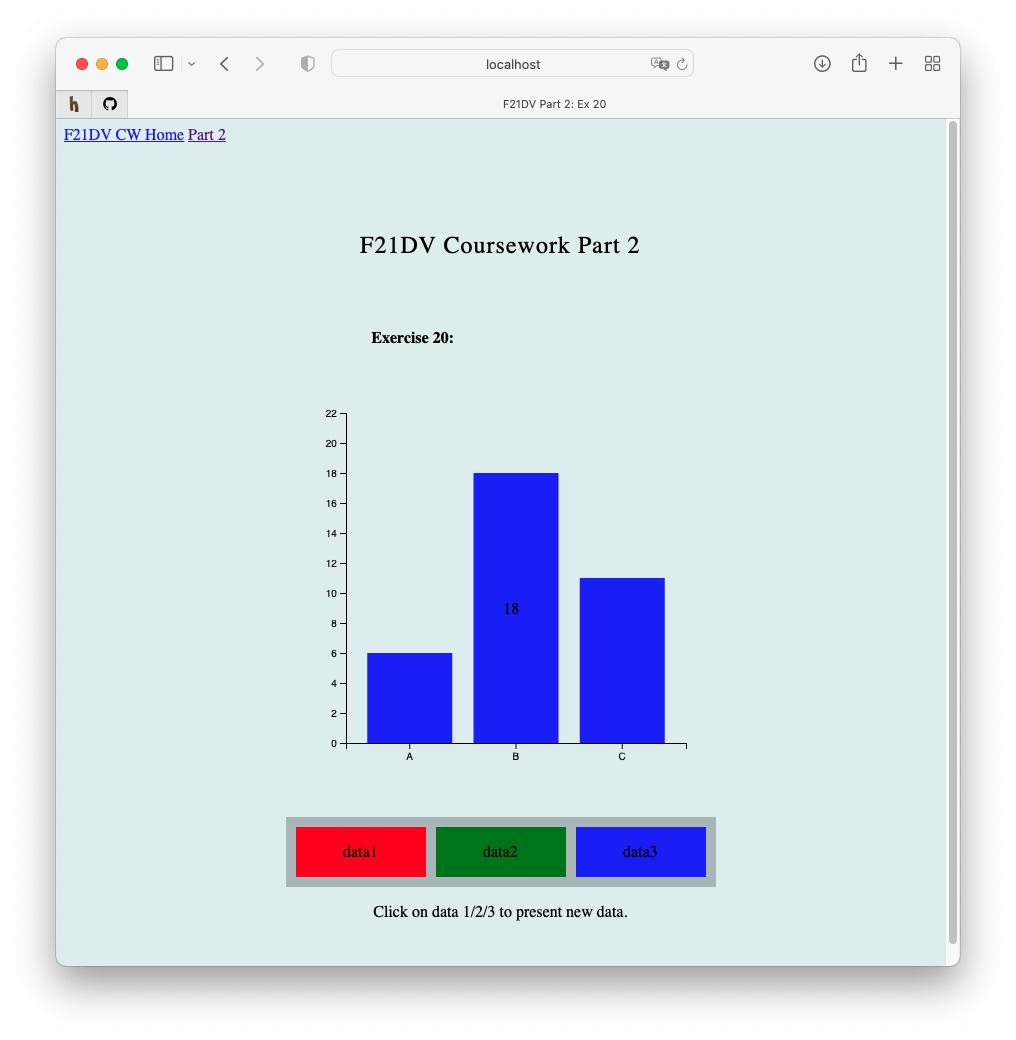
\includegraphics[width = 7.5cm]{images/ex20.png}
    % \includegraphics[width = 7.5cm]{images/ex18_2.png}
    % \includegraphics[width = 7.5cm]{images/ex18_3.png}
    % \includegraphics[width = 7.5cm]{images/ex17_4.png}
    \label{fig:ex20}
    \caption{Exercise 20}
\end{figure}
\FloatBarrier
% \lstinputlisting[language=JavaScript]{../../public/js/part2/task18.js}
Figure \ref{fig:ex20} shows the same bar chart, just that I have now added a mouse over function to show the actual value of the bars upon hover.

\newpage
\section{Exercise 21}
\begin{figure}[!ht]
    \centering
    \includegraphics[width = 7.5cm]{images/ex21.png}
    % \includegraphics[width = 7.5cm]{images/ex18_2.png}
    % \includegraphics[width = 7.5cm]{images/ex18_3.png}
    % \includegraphics[width = 7.5cm]{images/ex17_4.png}
    \label{fig:ex21}
    \caption{Exercise 21}
\end{figure}
\FloatBarrier
% \lstinputlisting[language=JavaScript]{../../public/js/part2/task18.js}
Figure \ref{fig:ex21} shows the same bar chart as before, except that there is now an extra axis on top and on the right of the svg.

\newpage
\section{Exercise 22}
\begin{figure}[!ht]
    \centering
    \includegraphics[width = 7.5cm]{images/ex22_1.png}
    \includegraphics[width = 7.5cm]{images/ex22_2.png}
    \includegraphics[width = 7.5cm]{images/ex22_3.png}
    % \includegraphics[width = 7.5cm]{images/ex17_4.png}
    \label{fig:ex22}
    \caption{Exercise 22}
\end{figure}
\FloatBarrier
% \lstinputlisting[language=JavaScript]{../../public/js/part2/task18.js}
Figure \ref{fig:ex22} shows the same bar chart as before, but now I have modified data 2 to contain an extra data entry. The transition here makes used og the \verb|.merge()| function and would help add the extra bar when needed, and would remove it when not in need, all these with annimation.

\newpage
\section{Exercise 23}
\begin{figure}[!ht]
    \centering
    \includegraphics[width = 7.5cm]{images/ex23_1.png}
    \includegraphics[width = 7.5cm]{images/ex23_2.png}
    \includegraphics[width = 7.5cm]{images/ex23_3.png}
    % \includegraphics[width = 7.5cm]{images/ex17_4.png}
    \label{fig:ex23}
    \caption{Exercise 23}
\end{figure}
\FloatBarrier
% \lstinputlisting[language=JavaScript]{../../public/js/part2/task23.js}
Figure \ref{fig:ex23} shows a line chart for data 1 on load. Upon clicking the data 2 button, the lines would transition using its datapoints to data 2. The axes would also transition, adding or removing values.

\newpage
\section{Exercise 24-26}
\begin{figure}[!ht]
    \centering
    \includegraphics[width = 7.5cm]{images/ex24.png}
    \includegraphics[width = 7.5cm]{images/ex25.png}
    \includegraphics[width = 7.5cm]{images/ex26.png}
    % \includegraphics[width = 7.5cm]{images/ex17_4.png}
    \label{fig:ex24}
    \caption{Exercise 24 to 26}
\end{figure}
\FloatBarrier
% \lstinputlisting[language=JavaScript]{../../public/js/part2/task23.js}
Figure \ref{fig:ex24} shows results of interpolation within \verb|d3|. Interpolation would interpolate between any interpolatable values to find the percentage point between values. Each example and its results are shown in the figure \ref{fig:ex24}.


\newpage
\section{Exercise 27}
\begin{figure}[!ht]
    \centering
    \includegraphics[width = 7.5cm]{images/ex27_1.png}
    \includegraphics[width = 7.5cm]{images/ex27_2.png}
    % \includegraphics[width = 7.5cm]{images/ex23_3.png}
    % \includegraphics[width = 7.5cm]{images/ex17_4.png}
    \label{fig:ex27}
    \caption{Exercise 27}
\end{figure}
\FloatBarrier
% \lstinputlisting[language=JavaScript]{../../public/js/part2/task27.js}
Figure \ref{fig:ex27} shows a hollow pie chart with data about Apple. Upon clicking the Lemon button, the pie chart would transition and show data on Lemon instead. This is done semalessly once again using the \verb|.merge()| function on the pie chart \verb|line| object.

\newpage
\section{Exercise 28}
\begin{figure}[!ht]
    \centering
    \includegraphics[width = 7.5cm]{images/ex28_1.png}
    \includegraphics[width = 7.5cm]{images/ex28_2.png}
    % \includegraphics[width = 7.5cm]{images/ex23_3.png}
    % \includegraphics[width = 7.5cm]{images/ex17_4.png}
    \label{fig:ex28}
    \caption{Exercise 28}
\end{figure}
\FloatBarrier
% \lstinputlisting[language=JavaScript]{../../public/js/part2/task27.js}
Figure \ref{fig:ex28} shows two randomised circles on an svg using d3 force layout. This will be different each time the page is bring loaded. This will be the same for all exercises 28 through 32. This is done by using the d3 \verb|.forceSimulation()| to created node values with radius and many other informnation (force simulation overwrites the nodes data). Then using these information, polulate the svg with circles.

\newpage
\section{Exercise 29}
\begin{figure}[!ht]
    \centering
    \includegraphics[width = 7.5cm]{images/ex29.png}
    % \includegraphics[width = 7.5cm]{images/ex28_2.png}
    % \includegraphics[width = 7.5cm]{images/ex23_3.png}
    % \includegraphics[width = 7.5cm]{images/ex17_4.png}
    \label{fig:ex29}
    \caption{Exercise 29}
\end{figure}
\FloatBarrier
% \lstinputlisting[language=JavaScript]{../../public/js/part2/task27.js}
Figure \ref{fig:ex29} shows identical for simulation from the previous exercise. Difference is this is now based off radius values from a \verb|.csv()| file, containing values $1, 1.2, 1.4, ...$. Hence each time the page would show circles with the same position and size upon load each time.

\newpage
\section{Exercise 30}
\begin{figure}[!ht]
    \centering
    \includegraphics[width = 7.5cm]{images/ex30_1.png}
    \includegraphics[width = 7.5cm]{images/ex30_2.png}
    % \includegraphics[width = 7.5cm]{images/ex23_3.png}
    % \includegraphics[width = 7.5cm]{images/ex17_4.png}
    \label{fig:ex30}
    \caption{Exercise 30}
\end{figure}
\FloatBarrier
% \lstinputlisting[language=JavaScript]{../../public/js/part2/task27.js}
Figure \ref{fig:ex30} shows similar force sumulation circles as before. This time, I have reduced the number of circles to improve simulation performance, and added a text box upon hover of each cirlce, displaying the circle data | the circle radius. This is shwon in the figure above, before mouse over and after mouse over.

\newpage
\section{Exercise 31}
\begin{figure}[!ht]
    \centering
    \includegraphics[width = 7.5cm]{images/ex31_1.png}
    \includegraphics[width = 7.5cm]{images/ex31_2.png}
    % \includegraphics[width = 7.5cm]{images/ex23_3.png}
    % \includegraphics[width = 7.5cm]{images/ex17_4.png}
    \label{fig:ex31}
    \caption{Exercise 31}
\end{figure}
\FloatBarrier
% \lstinputlisting[language=JavaScript]{../../public/js/part2/task27.js}
Figure \ref{fig:ex31} shows same force sumulation circles as before. This time, there is just an added colour change to mouse over and out events.

\newpage
\section{Exercise 32}
\begin{figure}[!ht]
    \centering
    \includegraphics[width = 7.5cm]{images/ex32.png}
    % \includegraphics[width = 7.5cm]{images/ex23_3.png}
    % \includegraphics[width = 7.5cm]{images/ex17_4.png}
    \label{fig:ex32}
    \caption{Exercise 32}
\end{figure}
\FloatBarrier
% \lstinputlisting[language=JavaScript]{../../public/js/part2/task27.js}
Figure \ref{fig:ex32} shows same force sumulation circles as before. This time, I have expeeimented with different forces types. Mainly, this shows the \verb|.force(`y', ...)| type.



\end{document}